% ======================================================================
% scrbookreportarticle.tex
% Copyright (c) Markus Kohm, 2001-2019
%
% This file is part of the LaTeX2e KOMA-Script bundle.
%
% This work may be distributed and/or modified under the conditions of
% the LaTeX Project Public License, version 1.3c of the license.
% The latest version of this license is in
%   http://www.latex-project.org/lppl.txt
% and version 1.3c or later is part of all distributions of LaTeX 
% version 2005/12/01 or later and of this work.
%
% This work has the LPPL maintenance status "author-maintained".
%
% The Current Maintainer and author of this work is Markus Kohm.
%
% This work consists of all files listed in manifest.txt.
% ----------------------------------------------------------------------
% scrbookreportarticle.tex
% Copyright (c) Markus Kohm, 2001-2019
%
% Dieses Werk darf nach den Bedingungen der LaTeX Project Public Lizenz,
% Version 1.3c, verteilt und/oder veraendert werden.
% Die neuste Version dieser Lizenz ist
%   http://www.latex-project.org/lppl.txt
% und Version 1.3c ist Teil aller Verteilungen von LaTeX
% Version 2005/12/01 oder spaeter und dieses Werks.
%
% Dieses Werk hat den LPPL-Verwaltungs-Status "author-maintained"
% (allein durch den Autor verwaltet).
%
% Der Aktuelle Verwalter und Autor dieses Werkes ist Markus Kohm.
% 
% Dieses Werk besteht aus den in manifest.txt aufgefuehrten Dateien.
% ======================================================================
%
% Chapter about scrbook, scrreprt, and scrartcl of the KOMA-Script guide
% Maintained by Markus Kohm
%
% ----------------------------------------------------------------------
%
% Kapitel über scrbook, scrreprt und scrartcl in der KOMA-Script-Anleitung
% Verwaltet von Markus Kohm
%
% ============================================================================

\KOMAProvidesFile{scrbookreportarticle.tex}
                 [$Date: 2019-12-06 10:38:10 +0100 (Fri, 06 Dec 2019) $
                  KOMA-Script guide (chapter: scrbook, scrreprt, scrartcl)]

\chapter{Die Hauptklassen \Class{scrbook}, \Class{scrreprt}, \Class{scrartcl}}
\labelbase{maincls}%
\BeginIndexGroup
\BeginIndex{Class}{scrbook}%
\BeginIndex{Class}{scrreprt}%
\BeginIndex{Class}{scrartcl}%

\AddSeeIndex{Anweisung}{gen}{\GuidecmdIndexShort}{cmd}%
\AddSeeIndex{Makro}{gen}{\GuidecmdIndexShort}{cmd}%
Die Hauptklassen des \KOMAScript-Pakets sind als Äquivalent zu den
\LaTeX-Standard"-klassen angelegt. Das bedeutet, dass zu den drei
Standardklassen \Class{book}\IndexClass{book}, \Class{report}%
\IndexClass{report} und \Class{article}\IndexClass{article} im
\KOMAScript-Paket Entsprechungen zu finden sind. Daneben ist auch für die
Standardklasse \Class{letter}\IndexClass{letter} eine Entsprechung vorhanden.
Der Briefklasse in {\KOMAScript} ist jedoch ein eigenes Kapitel gewidmet, da
sie sich von den drei Hauptklassen grundsätzlich unterscheidet (siehe
\autoref{cha:scrlttr2}).

Die einfachste Möglichkeit, anstelle einer Standardklasse eine
\KOMAScript-Klasse zu verwenden, ist das Ersetzen des Klassennamens in der
Anweisung \verb|\documentclass| entsprechend
\autoref{tab:maincls.overview}. Man tauscht
also beispielsweise \Macro{documentclass}\PParameter{article} gegen
\Macro{documentclass}\PParameter{scrartcl}. Der anschließende \LaTeX-Lauf
sollte lediglich einige Layoutänderungen mit sich bringen. Ein großer Teil der
in den nachfolgenden Abschnitten beschriebenen vielfältigen Möglichkeiten und
Optionen werden von den \KOMAScript-Klassen zusätzlich geboten.

\begin{table}
%  \centering
  \KOMAoptions{captions=topbeside}%
  \setcapindent{0pt}%
%  \caption
  \begin{captionbeside}
  [Klassengegenüberstellung]{\label{tab:maincls.overview}Gegenüberstellung der
    Standardklassen und der \KOMAScript-Klassen}
  [l]
  \begin{tabular}[t]{ll}
    \toprule
    Standard-Klasse & \KOMAScript-Klasse \\%& \Script-Stil (\LaTeX2.09)\\
    \midrule
    \Class{article} & \Class{scrartcl}   \\%& \File{script\textunderscore s} \\
    \Class{report}  & \Class{scrreprt}   \\%& \File{script}   \\
    \Class{book}    & \Class{scrbook}    \\%& \File{script}   \\
    \Class{letter}  & \Class{scrlttr2}   \\%& \File{script\textunderscore l} \\
    \bottomrule
  \end{tabular}
  \end{captionbeside}
\end{table}

Es sei an dieser Stelle jedoch nicht verschwiegen, dass einige Paketautoren
ihre Pakete auf Basis der Implementierung und sogar von internem Code der
Standardklassen entwickeln und dabei keine Rücksicht auf komplett unabhängige
Entwicklungen wie die \KOMAScript-Klassen nehmen. In solchen Fällen kann es
beim ersten \LaTeX-Lauf nach der Umstellung durchaus zu Fehlermeldungen oder
zusäzlichen Warnungen kommen. Meist lassen sich diese auf einfache Weise
beheben. Oftmals können dazu die erweiterten Möglichkeiten von \KOMAScript{}
genutzt werden, wodurch das problematische Paket dann vollständig
entfällt. Manchmal kann auch das in \autoref{cha:scrhack} ab Seite
\autopageref{cha:scrhack} dokumentierte \hyperref[cha:scrhack]{Paket
  \Package{scrhack}}\IndexPackage{scrhack} Abhilfe schaffen. Auch der Ersatz
von veralteten Paketen durch aktuelle Nachfolger kann zur Beseitigung
derartiger Probleme beitragen. Teilweise geben sogar die \KOMAScript-Klassen
durch entsprechende Warnungen Hilfestellung bei der Lösung von
Inkompatibilitäten.

Lassen Sie mich der Erläuterung der Klassen noch eine Bemerkung
vorausschicken. Oft ist man sich am Anfang eines Dokuments unsicher, welche
Einstellungen konkret zu wählen sind.  Bei einigen Einstellungen, wie der
Auswahl des Papierformats, mögen sie bereits vorab feststehen. Aber schon die
Frage nach der Seitenauf"|teilung könnte im Voraus schwer zu beantworten sein.
Andererseits sollten diese Angaben für die Haupttätigkeiten des Autors --
Entwurf der Gliederung, Schreiben des Textes, Zusammenstellen von Abbildungen,
Tabellen und Verzeichnissen -- zunächst auch unerheblich sein. Konzentrieren
Sie sich als Autor erst einmal auf den Inhalt. Wenn der dann steht, können Sie
sich um die Feinheiten der Form kümmern. Neben der Auswahl der Optionen
gehören dazu dann auch Dinge wie die Korrektur der Trennung und möglicherweise
dezente Eingriffe in den Seitenumbruch oder die Verteilung von Abbildungen und
Tabellen.


% %%%%%%%%%%%%%%%%%%%%%%%%%%%%%%%%%%%%%%%%%%%%%%%%%%%%%%%%%%%%%%%%%%%%%%

\LoadCommonFile{options} % \section{Frühe oder späte Optionenwahl}

%\iffree{}{\clearpage}% Umbruchkorrektur!!!

\LoadCommonFile{compatibility} % \section{Kompatibilität zu früheren Versionen von \KOMAScript}

\LoadCommonFile{draftmode} % \section{Entwurfsmodus}

\LoadCommonFile{typearea} % \section{Seitenauf"|teilung}

\begin{Declaration}
  \Macro{flushbottom}
  \Macro{raggedbottom}
\end{Declaration}
\begin{Explain}
  Insbesondere bei doppelseitigen Dokumenten ist es wünschenswert, wenn nicht
  nur alle ersten Zeilen eines Satzspiegels mit ihrer Grundlinie auf der
  gleichen Höhe liegen, sondern auch die letzten Zeilen einer
  Doppelseite. Enthält eine Seite nur Text ohne Absätze und Überschriften, so
  hat man das automatisch, wenn bei der Konstruktion des Satzspiegels einige
  Grundregeln befolgt wurden. Aber bereits dann, wenn Absätze mit einem halben
  Grundlinienabstand markiert werden, genügt es, wenn die Anzahl der Absätze
  auf der einen Seite um eine ungerade Zahl von der auf der anderen Seite
  abweicht, damit dieses Ziel nicht mehr erreicht werden kann. Es ist dann
  notwendig, dass man zumindest einige der vertikalen Abstände etwas dehnt
  oder staucht, um das Ziel wieder zu erreichen. \TeX{} kennt zu diesem Zweck
  dehn- und stauchbare Abstände und \LaTeX{} bietet die Möglichkeit,
  diesen \emph{vertikalen Ausgleich}\Index{Ausgleich} automatisch
  durchzuführen.
\end{Explain}

Wird über die Option
\Option{twoside}\IndexOption{twoside}\important{\Option{twoside}} (siehe
\autoref{sec:typearea.typearea}, \DescPageRef{typearea.option.twoside})
doppelseitiger oder über Option
\Option{twocolumn}\IndexOption{twocolumn}\important{\Option{twocolumn}} (siehe
\DescPageRef{typearea.option.twocolumn}) zweispaltiger Satz angefordert, so
wird der vertikale Ausgleich ebenfalls
eingeschaltet. Das\ChangedAt{v3.17}{\Class{scrbook}\and \Class{scrreprt}\and
  \Class{scrartcl}} gilt jedoch bei einer Kompatibilitätseinstellung zu einer
\KOMAScript-Version vor 3.17 (siehe
\autoref{sec:\LabelBase.compatibilityOptions},
\DescPageRef{\LabelBase.option.version}, Option
\DescRef{\LabelBase.option.version}%
\IndexOption{version}\important{\OptionValueRef{\LabelBase}{version}{3.17}})
nicht, wenn die Option über \DescRef{\LabelBase.cmd.KOMAoption} oder
\DescRef{\LabelBase.cmd.KOMAoptions} geändert wird.

Man kann den vertikalen Ausgleich auch mit \Macro{flushbottom} jederzeit
ab der aktuellen Seite explizit fordern. Umgekehrt ist es möglich, mit
\Macro{raggedbottom} den vertikalen Ausgleich ab der aktuellen Seite explizit
abzuschalten. Dies entspricht der Voreinstellung bei einseitigem Satz.

{\KOMAScript} verwendet übrigens einen leicht modifizierten Verzicht auf den
vertikalen Ausgleich. \iffree{}{Näheres dazu ist in
  \autoref{sec:maincls-experts.addInfos},
  \DescPageRef{maincls-experts.cmd.footnoterule} zu erfahren.}%
%
\EndIndexGroup
%
\EndIndexGroup


\LoadCommonFile{fontsize} % \section{Wahl der Schriftgröße für das Dokument}

\LoadCommonFile{textmarkup} % \section{Textauszeichnungen}

\LoadCommonFile{titles}% \section{Dokumenttitel}

\section{Zusammenfassung}
\seclabel{abstract}
\BeginIndexGroup
\BeginIndex{}{Zusammenfassung}%

Insbesondere bei Artikeln%
\iffalse % Umbruchkorrektur
, seltener bei Berichten findet man unmittelbar unter der Titelei und noch vor
dem Inhaltsverzeichnis %
\else %
\ findet man zwischen Titel und Inhaltsverzeichnis oft %
\fi %
eine Zusammenfassung.  Bei Verwendung eines Titelkopfes ist die
Zusammenfassung in der Regel %
\iffalse % Umbruchkorrektur
ein rechts und links eingezogener Block. %
\else %
rechts und links eingezogen. %
\fi %
\iffalse % Umbruchkorrektur
Im Vergleich dazu wird bei Verwendung von Titelseiten %
\else %
Bei Verwendung von Titelseiten wird %
\fi %
die Zusammenfassung eher als Kapitel oder Abschnitt gesetzt.

\begin{Declaration}
  \OptionVName{abstract}{Ein-Aus-Wert}
\end{Declaration}%
Bei\ChangedAt{v3.00}{\Class{scrreprt}\and \Class{scrartcl}}%
\OnlyAt{\Class{scrreprt}\and \Class{scrartcl}} den
Standardklassen\textnote{\KOMAScript{} vs. Standardklassen} setzt die
\DescRef{\LabelBase.env.abstract}-Umgebung noch den zentrierten Titel
»\abstractname« vor die Zusammenfassung. Früher war dies durchaus
üblich. Inzwischen sind wir durch das Zeitunglesen darin geübt, einen
entsprechend hervorgehobenen Text am Anfang eines Artikels oder Berichts als
Zusammenfassung zu erkennen. Dies gilt umso mehr, wenn dieser Text noch vor
dem Inhaltsverzeichnis steht.  Zudem verwundert es, wenn ausgerechnet diese
Überschrift klein und zentriert ist. {\KOMAScript} bietet mit der Option
\Option{abstract} die Möglichkeit, die Überschrift über der Zusammenfassung
ein- oder auszuschalten.  Als \PName{Ein-Aus-Wert} kann einer der
Standardwerte für einfache Schalter aus \autoref{tab:truefalseswitch},
\autopageref{tab:truefalseswitch} verwendet werden. Voreingestellt ist bei
\KOMAScript{} \PValue{false}.

Bei Büchern wird in der Regel eine andere Art der Zusammenfassung
verwendet. Dort setzt man ein entsprechendes Kapitel an den Anfang oder das
Ende des Werks.  Oft wird diese Zusammenfassung entweder mit der Einleitung
oder einem weiteren Ausblick verknüpft. Daher gibt es bei \Class{scrbook}
überhaupt keine \DescRef{\LabelBase.env.abstract}-Umgebung.
Bei\textnote{Tipp!}  Berichten im weiteren Sinne, etwa einer Studien- oder
Diplomarbeit, ist ebenfalls eine Zusammenfassung in dieser Form zu
empfehlen. Siehe dazu die in \autoref{sec:maincls.structure}, ab
\DescPageRef{\LabelBase.cmd.chapter*} dokumentierten Befehle
\DescRef{\LabelBase.cmd.chapter*}\IndexCmd{chapter*}.
\DescRef{\LabelBase.cmd.addchap}\IndexCmd{addchap} und
\DescRef{\LabelBase.cmd.addchap*}\IndexCmd{addchap*}.%
\EndIndexGroup


\begin{Declaration}
  \begin{Environment}{abstract}\end{Environment}
\end{Declaration}%
\OnlyAt{\Class{scrartcl}\and \Class{scrreprt}}%
Einige \LaTeX-Klassen bieten eine spezielle Umgebung für die
Zusammenfassung: die \Environment{abstract}-Umgebung. Diese wird unmittelbar
ausgegeben, ist also nicht Bestandteil der mit
\DescRef{\LabelBase.cmd.maketitle} gesetzten Titelei. Bitte\textnote{Achtung!}
beachten Sie unbedingt, dass es sich bei \Environment{abstract} um eine
Umgebung und nicht um eine Anweisung handelt. Ob die Zusammenfassung mit einer
Überschrift versehen wird oder nicht, wird über die Option
\DescRef{\LabelBase.option.abstract} gesteuert (siehe oben).

Bei Büchern ist die Zusammenfassung häufig Bestandteil der Einleitung oder
eines gesonderten Kapitels am Ende des Dokuments. Daher gibt es bei
\Class{scrbook} keine \Environment{abstract}-Umgebung.  Bei Verwendung der
Klasse \Class{scrreprt} ist es sicher eine Überlegung wert, ob man nicht
genauso verfahren sollte. Siehe hierzu in \autoref{sec:\LabelBase.structure}
ab \DescPageRef{\LabelBase.cmd.chapter*}
die Anweisungen \DescRef{\LabelBase.cmd.chapter*}\IndexCmd{chapter*} und
\DescRef{\LabelBase.cmd.addchap}\IndexCmd{addchap} oder
\DescRef{\LabelBase.cmd.addchap*}.% (\DescPageRef{\LabelBase.cmd.addchap}).

Wird ein Titelkopf\Index{Titel>Kopf} (siehe Option
\DescRef{\LabelBase.option.titlepage}, \autoref{sec:\LabelBase.titlepage},
\DescPageRef{\LabelBase.option.titlepage}) verwendet, so wird die
Zusammenfassung intern mit Hilfe einer
\DescRef{\LabelBase.env.quotation}-Umgebung\IndexEnv{quotation} (siehe
\autoref{sec:\LabelBase.lists}, \DescPageRef{\LabelBase.env.quotation})
gesetzt. Dabei werden Absatzanfänge normalerweise mit Einzug gesetzt. Soll der
erste Absatz nicht eingezogen werden, so kann dieser Einzug mit
\Macro{noindent}\IndexCmd{noindent}\important{\Macro{noindent}}
\iffree{unmittelbar nach \Macro{begin}\PParameter{abstract}}{am Anfang der
  Umgebung} unterdrückt werden.%
%
\EndIndexGroup
%
\EndIndexGroup


\section{Inhaltsverzeichnis}
\seclabel{toc}
\BeginIndexGroup
\BeginIndex{}{Inhaltsverzeichnis}

Auf die Titelei und eine eventuell vorhandene Zusammenfassung folgt
normalerweise das Inhaltsverzeichnis. Häufig findet
man nach dem Inhaltsverzeichnis auch noch die Verzeichnisse der
Gleitumgebungen, beispielsweise von Tabellen und Abbildungen (siehe
\autoref{sec:\LabelBase.floats}).

\iffalse%
Es ist zu beachten, dass neben den in diesem Abschnitt dokumentierten
Möglichkeiten auch noch die Anweisungen
\DescRef{maincls-experts.cmd.DeclareSectionCommand},
\DescRef{maincls-experts.cmd.DeclareNewSectionCommand},
\DescRef{maincls-experts.cmd.RedeclareSectionCommand} und
\DescRef{maincls-experts.cmd.ProvideSectionCommand} Auswirkungen auf das
Inhaltsverzeichnis haben können. Siehe \autoref{sec:maincls-experts.sections},
\DescPageRef{maincls-experts.cmd.DeclareSectionCommand}.%
\else%
Neben den in diesem Abschnitt dokumentierten Möglichkeiten hat auch der mit
\DescRef{tocbasic.cmd.DeclareTOCStyleEntry}\IndexCmd{DeclareTOCStyleEntry}%
\important[O]{\DescRef{tocbasic.cmd.DeclareTOCStyleEntry}}
gewählte und
konfigurierte Eintragsstil des Pakets
\hyperref[cha:tocbasic]{\Package{tocbasic}}%
\important{\hyperref[cha:tocbasic]{\Package{tocbasic}}}%
\IndexPackage{tocbasic} (siehe
\DescPageRef{tocbasic.cmd.DeclareTOCStyleEntry}) maßgeblichen Einfluss auf die
Darstellung des Inhaltsverzeichnisses. Entsprechend können sich auch die in
\autoref{sec:maincls-experts.sections} ab
\DescPageRef{maincls-experts.cmd.DeclareSectionCommand} dokumentierten
Befehle
\DescRef{maincls-experts.cmd.DeclareSectionCommand}%
\important[O]{\DescRef{maincls-experts.cmd.DeclareSectionCommand}}%
\IndexCmd{DeclareSectionCommand},
\DescRef{maincls-experts.cmd.ProvideSectionCommand}%
\IndexCmd{ProvideSectionCommand},
\DescRef{maincls-experts.cmd.DeclareNewSectionCommand}%
\IndexCmd{DeclareNewSectionCommand} und
\DescRef{maincls-experts.cmd.RedeclareSectionCommand}%
\IndexCmd{RedeclareSectionCommand} auf das Inhaltsverzeichnis auswirken.%
\fi


\begin{Declaration}
  \OptionVName{toc}{Einstellung}
\end{Declaration}
Neuerdings ist es fast schon üblich geworden Tabellen- und
Abbildungsverzeichnis sowie das Literaturverzeichnis, seltener das
Stichwortverzeichnis, ins Inhaltsverzeichnis aufzunehmen. Dies hat sicher auch
mit der neuen Mode zu tun, Abbildungs- und Tabellenverzeichnis ans Buchende zu
stellen. Beide Verzeichnisse haben von Aufbau und Intention eine deutliche
Ähnlichkeit mit dem Inhaltsverzeichnis.  Daher betrachte ich die Entwicklung
skeptisch. Da\important{\OptionValue{toc}{listof}} es keinen Sinn hat, nur das
Tabellen- oder nur das Abbildungsverzeichnis ohne das jeweils andere ins
Inhaltsverzeichnis aufzunehmen, werden mit der
\PName{Einstellung}\ChangedAt{v3.00}{\Class{scrbook}\and \Class{scrreprt}\and
  \Class{scrartcl}} \PValue{listof}\IndexOption{toc~=\textKValue{listof}} beide
Verzeichnisse gemeinsam ins Inhaltsverzeichnis aufgenommen. Dabei werden auch
Verzeichnisse berücksichtigt, die mit Hilfe des
\Package{float}-Pakets\IndexPackage{float} ab Version~1.2e (siehe
\cite{package:float}) oder \Package{floatrow} (siehe \cite{package:floatrow})
erstellt werden. Als\important{\OptionValue{toc}{listofnumbered}}
Verzeichnisse, die den Inhalt anderer Abschnitte des Werks auf"|führen,
erhalten Tabellen"~, Abbildungs- und die mit den genannten Paketen erzeugten
Verzeichnisse grundsätzlich keine Kapitelnummer. Wer diesen Grundsatz
ignorieren will, bedient sich der \PName{Einstellung}
\PValue{listofnumbered}\IndexOption{toc~=\textKValue{listofnumbered}}.

\leavevmode\LabelOptionValue{toc}{index}\nobreak
Das\important{\OptionValue{toc}{index}} Stichwortverzeichnis erhält mit
\OptionValue{toc}{index}\IndexOption{toc~=\textKValue{index}} einen Eintrag im
Inhaltsverzeichnis. Da das Stichwortverzeichnis ebenfalls nur Verweise auf den
Inhalt anderer Abschnitte enthält, wird auch dieser Eintrag grundsätzlich
nicht nummeriert. Eine\ChangedAt{v3.18}{\Class{scrbook}\and
  \Class{scrreprt}\and \Class{scrartcl}}
Abweichung\important{\OptionValue{toc}{indexnumbered}} von diesem Grundsatz
wird von \KOMAScript{} trotz Bedenken des Autors mit
\OptionValue{toc}{indexnumbered}\IndexOption{toc~=\textKValue{indexnumbered}}
ebenfalls unterstützt.

\leavevmode\LabelOptionValue{toc}{bibliography}\nobreak Das
Literaturverzeichnis stellt eine etwas andere Art von Verzeichnis dar. Hier
wird nicht der Inhalt des vorliegenden Werks aufgelistet, sondern auf externe
Inhalte verwiesen. Mit\important{\OptionValue{toc}{bibliographynumbered}}
dieser Begründung könnte man argumentieren, dass das Literaturverzeichnis ein
eigenes Kapitel bzw. einen eigenen Abschnitt darstelle und somit eine Nummer
verdiene.  Die Option \OptionValue{toc}{bibliographynumbered}%
\IndexOption{toc~=\textKValue{bibliographynumbered}} führt genau dazu,
einschließlich des dann fälligen Eintrags im Inhaltsverzeichnis.  Ich selbst
bin allerdings der Meinung, dass bei dieser Argumentation auch ein
klassisches, kommentiertes Quellenverzeichnis ein eigenes Kapitel
wäre. Außerdem ist das Literaturverzeichnis letztlich nichts, was man selbst
geschrieben hat. Deshalb\important{\OptionValue{toc}{bibliography}} erscheint
mir allenfalls ein nicht nummerierter Eintrag im Inhaltsverzeichnis
angemessen, was mit der Einstellung
\OptionValue{toc}{bibliography}\IndexOption{toc~=\textKValue{bibliography}}
erreicht wird.

\leavevmode\LabelOptionValue{toc}{graduated}\nobreak
Normalerweise\ChangedAt{v2.8q}{%
  \Class{scrbook}\and \Class{scrreprt}\and \Class{scrartcl}}%
\important{\OptionValue{toc}{graduated}} wird das Inhaltsverzeichnis so
formatiert, dass die Gliederungsebenen unterschiedlich weit eingezogen
werden. Dabei wird für die Gliederungsnummer jeder Ebene ein Raum fester
Breite vorgesehen, in dem die Nummer linksbündig gesetzt wird. Dies entspricht
der Einstellung\ChangedAt{v3.00}{\Class{scrbook}\and \Class{scrreprt}\and
  \Class{scrartcl}}
\OptionValue{toc}{graduated}\IndexOption{toc~=\textKValue{graduated}}.

\leavevmode\LabelOptionValue{toc}{flat}\nobreak
Werden sehr viele Gliederungspunkte verwendet, so werden die
Gliederungsnummern sehr breit. Damit reicht der vorgesehene Platz nicht
aus. In \cite{DANTE:FAQ} wird für solche Fälle vorgeschlagen, die Erzeugung
des Inhaltsverzeichnisses
umzudefinieren. \KOMAScript{}\important{\OptionValue{toc}{flat}} bietet jedoch
eine alternative Formatierung an, bei der das Problem nicht auf"|tritt. Bei
Verwendung der Option \OptionValue{toc}{flat}\IndexOption{toc~=\textKValue{flat}}
werden die unterschiedlichen Gliederungsebenen nicht unterschiedlich weit
eingezogen. Stattdessen wird eine tabellenartige Form gewählt, in der alle
Gliederungsnummern und alle Gliederungstexte jeweils in einer Spalte
linksbündig untereinander stehen. Der für die Gliederungsnummern benötigte
Platz wird dabei automatisch ermittelt.

Einen Überblick über alle möglichen Werte für die \PName{Einstellung} von
\Option{toc} ist in \autoref{tab:maincls.toc} zu finden.

\begin{desclist}
  \desccaption[{Mögliche Werte für Option \Option{toc}}]{%
    Mögliche Werte für Option \Option{toc} zur Einstellung von Form und Inhalt
    des Inhaltsverzeichnisses\label{tab:maincls.toc}%
  }{%
    Mögliche Werte für Option \Option{toc} (\emph{Fortsetzung})%
  }%
  \entry{\PValue{bibliography}, \PValue{bib}}{%
    Das Literaturverzeichnis erhält einen Eintrag im Inhaltsverzeichnis, ohne
    dass es nummeriert wird.%
    \IndexOption{toc~=\textKValue{bibliography}}}%
  \entry{\PValue{bibliographynumbered}, \PValue{bibnumbered},
    \PValue{numberedbibliography}, \PValue{numberedbib}}{%
    Das Literaturverzeichnis erhält einen Eintrag im Inhaltsverzeichnis und
    wird nummeriert.%
    \IndexOption{toc~=\textKValue{bibliographynumbered}}}%
  \entry{\PValue{chapterentrywithdots}, \PValue{chapterentrydotfill}}{%
    \ChangedAt[2014/12]{v3.15}{\Class{scrbook}\and \Class{scrreprt}}%
    Bei den Kapiteleinträgen der Klassen \Class{scrbook} und \Class{scrreprt}
    werden Text und Seitenzahl ebenfalls durch eine punktierte Linie
    miteinander verbunden.%
    \IndexOption{toc~=\textKValue{chapterentrywithdots}}}%
  \entry{\PValue{chapterentrywithoutdots}, \PValue{chapterentryfill}}{%
    \ChangedAt{v3.15}{\Class{scrbook}\and \Class{scrreprt}}%
    Bei den Kapiteleinträgen der Klassen \Class{scrbook} und \Class{scrreprt}
    werden Text und Seitenzahl nicht durch eine punktierte Linie miteinander
    verbunden. Dies entspricht der Voreinstellung.%
    \IndexOption{toc~=\textKValue{chapterentrywithoutdots}}}%
  \entry{\PValue{flat}, \PValue{left}}{%
    Das Inhaltsverzeichnis erhält eine tabellarische Form. Die
    Gliederungsnummern sind dabei die erste Spalte, die Überschriften die
    zweite Spalte, die Seitenzahlen die dritte Spalte. Der Platz, der für die
    Gliederungsnummern reserviert wird, richtet sich nach dem benötigten Platz
    des vorherigen \LaTeX-Laufs.%
    \IndexOption{toc~=\textKValue{flat}}}%
  \entry{\PValue{graduated}, \PValue{indent}, \PValue{indented}}{%
    Das Inhaltsverzeichnis erhält eine hierarchische Form. Es steht nur ein
    begrenzter Platz für die Gliederungsnummern zur Verfügung. Dies entspricht
    der Voreinstellung.%
    \IndexOption{toc~=\textKValue{graduated}}}%
  \entry{\PValue{indenttextentries}, \PValue{indentunnumbered},
    \PValue{numberline}}{%
    \ChangedAt{v3.12}{\Class{scrbook}\and \Class{scrreprt}\and
      \Class{scrartcl}}%
    Die Eigenschaft \PValue{numberline} (siehe \autoref{sec:tocbasic.toc},
    \DescPageRef{tocbasic.cmd.setuptoc}) wird für das Inhaltsverzeichnis
    gesetzt. Dadurch werden nicht nummerierte Einträge linksbündig mit dem
    Text von nummerierten Einträgen gleicher Ebene gesetzt.%
    \IndexOption{toc~=\textKValue{numberline}}}%
  \entry{\PValue{index}, \PValue{idx}}{%
    Das Stichwortverzeichnis erhält einen Eintrag im Inhaltsverzeichnis, ohne
    dass es nummeriert wird.%
    \IndexOption{toc~=\textKValue{index}}}%
  \entry{\PValue{indexnumbered}, \PValue{idxnumbered}, \PValue{numberedindex},
    \PValue{numberedidx}}{%
    \ChangedAt{v3.18}{\Class{scrbook}\and \Class{scrreprt}\and
      \Class{scrartcl}}%
    Das Stichwortverzeichnis erhält einen Eintrag im Inhaltsverzeichnis und
    wird nummeriert.%
    \IndexOption{toc~=\textKValue{index}}}%
  \entry{\PValue{leftaligntextentries}, \PValue{leftalignunnumbered},
    \PValue{nonumberline}}{%
    \ChangedAt{v3.12}{\Class{scrbook}\and \Class{scrreprt}\and
      \Class{scrartcl}}%
    Die Eigenschaft \PValue{numberline} (siehe \autoref{sec:tocbasic.toc},
    \DescPageRef{tocbasic.cmd.setuptoc}) wird für das Inhaltsverzeichnis
    gelöscht. Dadurch werden nicht nummerierte Einträge linksbündig mit der
    Nummer von nummerierten Einträgen gleicher Ebene gesetzt. Dies entspricht
    der Voreinstellung.%
    \IndexOption{toc~=\textKValue{numberline}}}%
  \pventry{listof}{%
    Die Verzeichnisse der Gleitumgebungen, beispielsweise das Abbildungs"~ und
    das Tabellenverzeichnis, erhalten einen Eintrag im Inhaltsverzeichnis,
    ohne dass sie nummeriert werden.%
    \IndexOption{toc~=\textKValue{listof}}}%
  \entry{\PValue{listofnumbered}, \PValue{numberedlistof}}{%
    Die Verzeichnisse der Gleitumgebungen, beispielsweise das Abbildungs"~ und
    das Tabellenverzeichnis, erhalten einen Eintrag im Inhaltsverzeichnis und
    werden nummeriert.%
    \IndexOption{toc~=\textKValue{listofnumbered}}}%
  \entry{\PValue{nobibliography}, \PValue{nobib}}{%
    Das Literaturverzeichnis erhält keinen Eintrag im Inhaltsverzeichnis. Dies
    entspricht der Voreinstellung.%
    \IndexOption{toc~=\textKValue{nobibliography}}}%
  \entry{\PValue{noindex}, \PValue{noidx}}{%
    Das Stichwortverzeichnis erhält keinen Eintrag im Inhaltsverzeichnis. Dies
    entspricht der Voreinstellung.%
    \IndexOption{toc~=\textKValue{noindex}}}%
  \pventry{nolistof}{%
    Die Verzeichnisse der Gleitumgebungen, beispielsweise das Abbildungs"~ und
    das Tabellenverzeichnis, erhalten keinen Eintrag im
    Inhaltsverzeichnis. Dies entspricht der Voreinstellung.%
    \IndexOption{toc~=\textKValue{nolistof}}}%
  \entry{\PValue{sectionentrywithdots}, \PValue{sectionentrydotfill}}{%
    \ChangedAt[2014/12]{v3.15}{\Class{scrartcl}}%
    Bei den Abschnittseinträgen der Klasse \Class{scrartcl} werden Text und
    Seitenzahl ebenfalls durch eine punktierte Linie miteinander verbunden.%
    \IndexOption{toc~=\textKValue{sectionentrywithdots}}}%
  \entry{\PValue{sectionentrywithoutdots}, \PValue{sectionentryfill}}{%
    \ChangedAt{v3.15}{\Class{scrartcl}}%
    Bei den Abschnittseinträgen der Klasse \Class{scrartcl} werden Text und
    Seitenzahl nicht durch eine punktierte Linie miteinander verbunden. Dies
    entspricht der Voreinstellung.%
    \IndexOption{toc~=\textKValue{sectionentrywithoutdots}}}%
\end{desclist}
%
\EndIndexGroup


\begin{Declaration}
  \OptionVName{chapterentrydots}{Ein-Aus-Wert}\\
  \OptionVName{sectionentrydots}{Ein-Aus-Wert}
\end{Declaration}
Diese\ChangedAt[2014/12]{v3.15}{\Class{scrbook}\and \Class{scrreprt}} Optionen
legen fest, ob im Inhaltsverzeichnis bei den Klassen \Class{scrbook} und
\Class{scrreprt}\OnlyAt{\Class{scrbook}\and \Class{scrreprt}} für die
Kapitelebene beziehungsweise bei der Klasse
\Class{scrartcl}\OnlyAt{\Class{scrartcl}} für die Abschnittsebene wie bei den
tieferen Ebenen auch eine punktierte Verbindungslinie zwischen dem Text des
Eintrags und der zugehörigen Seitenzahl verwendet werden soll. Als
\PName{Ein-Aus-Wert} kann einer der Standardwerte für einfache Schalter aus
\autoref{tab:truefalseswitch}, \autopageref{tab:truefalseswitch} verwendet
werden. Voreingestellt ist für beide Optionen \PValue{false}, wodurch statt
einer punktierten Linie lediglich ein Abstand verwendet wird.

\BeginIndex{FontElement}{chapterentrydots}\LabelFontElement{chapterentrydots}%
\BeginIndex{FontElement}{sectionentrydots}\LabelFontElement{sectionentrydots}%
Wird die punktierte Linie verwendet, so kann deren Schrift über das Element
\FontElement{chapterentrydots}%
\important{\FontElement{chapterentrydots}\\
  \FontElement{sectionentrydots}} oder \FontElement{sectionentrydots}
verändert werden (siehe \DescRef{\LabelBase.cmd.setkomafont} und
\DescRef{\LabelBase.cmd.addtokomafont}, \autoref{sec:\LabelBase.textmarkup},
\DescPageRef{\LabelBase.cmd.setkomafont}, sowie
\autoref{tab:maincls.fontelements},
\autopageref{tab:maincls.fontelements}). Die Voreinstellungen der Elemente
sind \autoref{tab:maincls.tocelements} auf
\autopageref{tab:maincls.tocelements} zu entnehmen. Es ist zu
beachten\textnote{Achtung!}, dass die Pünktchen nur sauber untereinander
stehen, wenn die Schrift aller Pünktchen identisch ist. Aus diesen Grund ist
die Ausgangschrift immer \Macro{normalfont}\Macro{normalsize}. Von
\DescRef{\LabelBase.fontelement.chapterentry} oder
\DescRef{\LabelBase.fontelement.sectionentry} bleibt für die Pünktchen daher
nur die Farbe erhalten.%
\EndIndexGroup


\begin{Declaration}
  \Macro{tableofcontents}
\end{Declaration}%
Die Ausgabe des Inhaltsverzeichnisses wird mit \Macro{tableofcontents}
erreicht. Um ein korrektes Inhaltsverzeichnis zu erhalten, sind nach jeder
Änderung mindestens zwei \LaTeX-Läufe notwendig. Mit der oben erläuterten
Option \DescRef{\LabelBase.option.toc} kann der Umfang und die Form des
Inhaltsverzeichnisses beeinflusst werden. Nach einer Umschaltung der Option
sind ebenfalls mindestens zwei weitere \LaTeX-Läufe notwendig.

Der Eintrag für \DescRef{\LabelBase.cmd.chapter}\IndexCmd{chapter} bei
\Class{scrbook}\IndexClass{scrbook} und \Class{scrreprt}\IndexClass{scrreprt}
beziehungsweise \DescRef{\LabelBase.cmd.section}\IndexCmd{section} bei
\Class{scrartcl}\IndexClass{scrartcl} sowie der Gliederungsebene
\DescRef{\LabelBase.cmd.part}\IndexCmd{part} wird nicht
eingerückt. Gleichzeitig befinden sich zwischen dem Text der Gliederungsebene
und der Seitenzahl in der Voreinstellung keine Pünktchen. Die typografischen
Gründe dafür liegen in der normalerweise anderen Schriftart sowie der
erwünschten Hervorhebung. Dies\ChangedAt{v3.15}{\Class{scrbook}\and
  \Class{scrreprt}\and \Class{scrartcl}} kann jedoch mit den zuvor
dokumentierten Optionen geändert werden. Das Inhaltsverzeichnis \iffree{dieser
  Anleitung}{dieses Buches} ist mit den Voreinstellungen gesetzt und dient als
Beispiel.

\BeginIndex{FontElement}{partentry}\LabelFontElement{partentry}%
\BeginIndex{FontElement}{chapterentry}\LabelFontElement{chapterentry}%
\BeginIndex{FontElement}{sectionentry}\LabelFontElement{sectionentry}%
Die\ChangedAt{v2.97c}{\Class{scrbook}\and \Class{scrreprt}\and
  \Class{scrartcl}}\important{\FontElement{partentry}\\
  \FontElement{chapterentry}\\
  \FontElement{sectionentry}} Schrift der oberen Inhaltsverzeichniseinträge
ist über die Elemente \FontElement{partentry} und für \Class{scrbook} und
\Class{scrreprt} über \FontElement{chapterentry} beziehungsweise
\FontElement{sectionentry} für \Class{scrartcl} einstellbar.
\BeginIndex{FontElement}{partentrypagenumber}%
\LabelFontElement{partentrypagenumber}%
\LabelFontElement{pagination}%
\BeginIndex{FontElement}{chapterentrypagenumber}%
\LabelFontElement{chapterentrypagenumber}%
\BeginIndex{FontElement}{sectionentrypagenumber}%
\LabelFontElement{sectionentrypagenumber}%
Die Schrift der Seitenzahlen kann jeweils davon abweichend über die Elemente
\FontElement{partentrypagenumber}%
\important{\FontElement{partentrypagenumber}} und
\FontElement{chapterentrypagenumber}%
\important{\FontElement{chapterentrypagenumber}\\
  \FontElement{sectionentrypagenumber}} (\Class{scrbook} und \Class{scrreprt})
beziehungsweise \FontElement{sectionentrypagenumber} (\Class{scrartcl})
eingestellt werden (siehe auch \DescRef{\LabelBase.cmd.setkomafont} und
\DescRef{\LabelBase.cmd.addtokomafont} in \autoref{sec:\LabelBase.textmarkup},
\DescPageRef{\LabelBase.cmd.setkomafont}, sowie
\autoref{tab:maincls.fontelements}, \autopageref{tab:maincls.fontelements}).
Werden\ChangedAt{v3.15}{\Class{scrbook}\and \Class{scrreprt}\and
  \Class{scrartcl}} je nach Klasse für die Kapitel- beziehungsweise
Abschnittseinträge ebenfalls punktierte Verbindungslinien zu den Seitenzahlen
über Option \DescRef{\LabelBase.option.toc}%
\IndexOption{toc~=\textKValue{chapterentrywithdots}}%
\IndexOption{toc~=\textKValue{sectionentrywithdots}},
\DescRef{\LabelBase.option.chapterentrydots}%
\IndexOption{chapterentrydots~=\PName{Ein-Aus-Wert}} oder
\DescRef{\LabelBase.option.sectionentrydots}%
\IndexOption{sectionentrydots~=\PName{Ein-Aus-Wert}} verwendet, so kann deren
Schrift über die Elemente \DescRef{\LabelBase.fontelement.chapterentrydots}%
\IndexFontElement{chapterentrydots}%
\important{\DescRef{\LabelBase.fontelement.chapterentrydots}\\
  \DescRef{\LabelBase.fontelement.sectionentrydots}} und
\DescRef{\LabelBase.fontelement.sectionentrydots}%
\IndexFontElement{sectionentrydots} verändert werden. Die Voreinstellungen der
Elemente sind \autoref{tab:maincls.tocelements} zu entnehmen.
\begin{table}
%  \centering
%  \caption
  \KOMAoptions{captions=topbeside}%
  \setcapindent{0pt}%
  \begin{captionbeside}
    [Schriftvoreinstellungen für die Elemente
      des Inhaltsverzeichnisses]
    {\label{tab:maincls.tocelements}%
      \hspace{0pt plus 1ex}Vorein\-stel\-lung\-en der Schrift für die Elemente
      des In\-halts\-ver\-zeich\-nis\-ses}
    [l]
    \setlength{\tabcolsep}{.9\tabcolsep}% Umbruchoptimierung!
  \begin{tabular}[t]{ll}
    \toprule
    Element & Voreinstellung \\
    \midrule
    \FontElement{partentry} &
    \DescRef{\LabelBase.cmd.usekomafont}\PParameter{disposition}\Macro{large} \\
    \FontElement{partentrypagenumber} & \\
    \FontElement{chapterentry} & \DescRef{\LabelBase.cmd.usekomafont}\PParameter{disposition}\\
    \FontElement{chapterentrydots} & \\
    \FontElement{chapterentrypagenumber} & \\
    \FontElement{sectionentry} & \DescRef{\LabelBase.cmd.usekomafont}\PParameter{disposition} \\
    \FontElement{sectionentrydots} & \\
    \FontElement{sectionentrypagenumber} & \\
    \bottomrule
  \end{tabular}
  \end{captionbeside}
\end{table}
%
\EndIndexGroup


\begin{Declaration}
  \Counter{tocdepth}
  \Macro{parttocdepth}
  \Macro{sectiontocdepth}
  \Macro{subsectiontocdepth}
  \Macro{subsubsectiontocdepth}
  \Macro{paragraphtocdepth}
  \Macro{subparagraphtocdepth}
\end{Declaration}%
Normalerweise werden bei den Klassen \Class{scrbook} und \Class{scrreprt} die
Gliederungsebenen \DescRef{\LabelBase.cmd.part} bis
\DescRef{\LabelBase.cmd.subsection} und bei der Klasse \Class{scrartcl} die
Ebenen \DescRef{\LabelBase.cmd.part} bis
\DescRef{\LabelBase.cmd.subsubsection} in das Inhaltsverzeichnis
aufgenommen. Dies wird über den Zähler \Counter{tocdepth} gesteuert.  Dabei
steht der Wert -1 für \DescRef{\LabelBase.cmd.part}, 0 für
\DescRef{\LabelBase.cmd.chapter} und so weiter.  Durch Setzen oder Erhöhen
oder Verringern des Zählers kann bestimmt werden, bis zu welcher
Gliederungsebene Einträge in das Inhaltsverzeichnis erfolgen sollen.  Dies ist
übrigens bei den Standardklassen ganz
genauso. Im\ChangedAt{v3.15}{\Class{scrbook}\and \Class{scrreprt}\and
  \Class{scrartcl}} Unterschied\textnote{\KOMAScript{} vs. Standardklassen} zu
den Standardklassen muss sich bei \KOMAScript{} aber niemand diese Zuordnung
merken. \KOMAScript{} definiert für jede Gliederungsebene eine Anweisung
\Macro{\PName{Ebene}tocdepth} mit dem entsprechenden Wert, die für Zuweisungen
an \Counter{tocdepth} verwendet werden kann.

Bitten beachten Sie\textnote{Achtung!}, dass die Werte für die Zähler
\Counter{tocdepth} und
\DescRef{\LabelBase.counter.secnumdepth}\IndexCounter{secnumdepth} (siehe
\autoref{sec:\LabelBase.structure},
\DescPageRef{\LabelBase.counter.secnumdepth}) bei
\Class{scrartcl}\OnlyAt{\Class{scrartcl}} für \DescRef{\LabelBase.cmd.part}
nicht übereinstimmen. Dies wurde aus Gründen der Kompatibilität von der
Standardklasse \Class{article} übernommen. Daher sollte beispielsweise die
Anweisung \DescRef{\LabelBase.cmd.partnumdepth}\IndexCmd{partnumdepth} auch
nicht zum Setzen von \Counter{tocdepth} verwendet werden.%
\begin{Example}
  Angenommen, Sie setzen einen Artikel, bei dem die Gliederungsebene
  \DescRef{\LabelBase.cmd.subsubsection} verwendet wird. Gehen wir weiter
  davon aus, dass Sie diese Gliederungsebene aber nicht im Inhaltsverzeichnis
  haben wollen. Dann könnte die Präambel Ihres Dokuments wie folgt
  aussehen:
\begin{lstcode}
  \documentclass{scrartcl}
  \setcounter{tocdepth}{\subsectiontocdepth}
\end{lstcode}
  Sie setzen den Zähler \Counter{tocdepth} daher auf den in Anweisung
  \Macro{subsectiontocdepth} gespeicherten Wert. Dass dies normalerweise der
  Wert 2 ist, müssen Sie sich also gar nicht merken.
  
  Wollen Sie stattdessen nur, dass eine Ebene weniger in das
  Inhaltsverzeichnis eingetragen wird als normalerweise, können Sie auch
  einfach vom voreingestellten Wert des Zählers \Counter{tocdepth} eins
  abziehen:
\begin{lstcode}
  \documentclass{scrartcl}
  \addtocounter{tocdepth}{-1}
\end{lstcode}
  Den\textnote{Tipp!} Wert, den Sie zu \Counter{tocdepth} addieren oder davon
  subtrahieren müssen, können Sie nach mindestens zwei \LaTeX-Läufen einfach
  im Inhaltsverzeichnis abzählen.
\end{Example}%
\EndIndexGroup
%
\EndIndexGroup


\LoadCommonFile{parmarkup}% \section{Absatzauszeichnung}

\LoadCommonFile{oddorevenpage}% \section{Erkennung von rechten und linken Seiten}


\section{Kopf und Fuß bei vordefinierten Seitenstilen}
\seclabel{pagestyle}

\BeginIndexGroup
\BeginIndex{}{Seiten>Stil}%
Eine der allgemeinen Eigenschaften eines Dokuments ist der Seitenstil. Bei
{\LaTeX} versteht man unter dem Seitenstil in erster Linie den Inhalt der
Kopf- und Fußzeilen.


\begin{Declaration}
  \OptionVName{headsepline}{Ein-Aus-Wert}
  \OptionVName{footsepline}{Ein-Aus-Wert}
\end{Declaration}%
Mit diesen Optionen kann eingestellt werden,
ob\ChangedAt{v3.00}{\Class{scrbook}\and \Class{scrreprt}\and \Class{scrartcl}}
unter Kolumnentiteln oder über dem Fuß eine horizontale Linie\Index{Trennlinie}
gewünscht wird. Als \PName{Ein-Aus-Wert} kann
einer der Standardwerte für einfache Schalter aus
\autoref{tab:truefalseswitch}, \autopageref{tab:truefalseswitch} verwendet
werden. Ein Aktivieren der Option \Option{headsepline} oder die Verwendung
der Option ohne Wertübergabe schaltet die Linie unter den Kolumnentiteln
ein. Ein Aktivieren der Option \Option{footsepline} oder die Verwendung der
Option ohne Wertübergabe schaltet die Linie über der Fußzeile ein. Die
Deaktivierung der Optionen schaltet die jeweilige Linie aus.

Bei\textnote{Achtung!} den weiter unten erklärten Seitenstilen
\DescRef{\LabelBase.pagestyle.empty} und \DescRef{\LabelBase.pagestyle.plain}
hat die Option \Option{headsepline} selbstverständlich keine Auswirkung, da
hier auf einen Seitenkopf\Index{Seiten>Kopf} ausdrücklich verzichtet werden
soll.  Typografisch betrachtet, hat eine solche Linie immer die Auswirkung,
dass der Kopf optisch näher an den Text heranrückt.  Dies bedeutet nun nicht,
dass der Kopf räumlich weiter vom Textkörper\Index{Text>Bereich} weggerückt
werden müsste.  Stattdessen sollte der Kopf dann bei der Berechnung des
Satzspiegels als zum Textkörper gehörend betrachtet werden. Dies wird bei
\KOMAScript{} dadurch erreicht, dass Paket
\hyperref[cha:typearea]{\Package{typearea}}%
\important{\hyperref[cha:typearea]{\Package{typearea}}}\IndexPackage{typearea}
ebenfalls auf \Option{headsepline} reagiert und automatisch die Paketoption
\DescRef{typearea.option.headinclude}%
\IndexOption{headinclude}\important{\DescRef{typearea.option.headinclude}} mit
gleichem Wert ausführt.  Entsprechendes gilt auch für die Fußlinie. Im
Gegensatz zu \Option{headsepline} wirkt sich die Option \Option{footsepline}
auch beim Seitenstil \PValue{plain} aus, da \PValue{plain} eine Seitenzahl im
Fuß ausgibt.

Die Optionen führen selbst keine automatische Neuberechnung des Satzspiegels
aus. Zur Neuberechnung des Satzspiegels siehe Option
\DescRef{typearea.option.DIV} mit den Werten
\hyperref[desc:typearea.option.DIV.last]{\PValue{last}} oder
\hyperref[desc:typearea.option.DIV.current]{\PValue{current}} (siehe
\DescPageRef{typearea.option.DIV.last}) oder die Anweisung
\DescRef{typearea.cmd.recalctypearea} (siehe
\DescPageRef{typearea.cmd.recalctypearea}) in \autoref{cha:typearea}.

Das Paket \hyperref[cha:scrlayer-scrpage]{\Package{scrlayer-scrpage}}%
\IndexPackage{scrlayer-scrpage}%
\important{\hyperref[cha:scrlayer-scrpage]{\Package{scrlayer-scrpage}}} (siehe
\autoref{cha:scrlayer-scrpage}) bietet weitere Einflussmöglichkeiten für
Linien im Kopf und Fuß.%
%
\EndIndexGroup


\begin{Declaration}
  \Macro{pagestyle}\Parameter{Seitenstil}
  \Macro{thispagestyle}\Parameter{lokaler Seitenstil}
\end{Declaration}%
Üblicherweise wird zwischen vier verschiedenen Seitenstilen unterschieden:
\begin{description}
\item[{\PageStyle{empty}%
    \BeginIndex[indexmain]{Pagestyle}{empty}\LabelPageStyle{empty}}] ist der
  Seitenstil, bei dem Kopf- und Fußzeile vollständig leer bleiben. Dies ist
  bei {\KOMAScript} vollkommen identisch zu den Standardklassen.%
\item[{\PageStyle{headings}%
    \BeginIndex[indexmain]{Pagestyle}{headings}\LabelPageStyle{headings}}] ist
  der Seitenstil für lebende Kolumnentitel. Das sind Kolumnentitel, bei denen
  Überschriften automatisch\Index[indexmain]{Kolumnentitel>automatisch} in den
  Seitenkopf übernommen werden. Im Internet oder in Beschreibungen zu
  \LaTeX-Paketen findet man auch häufig die englische Bezeichnung
  »\emph{running headline}«.  \OnlyAt{\Class{scrbook}\and \Class{scrreprt}}%
  Bei den Klassen \Class{scrbook}\IndexClass{scrbook} und
  \Class{scrreprt}\IndexClass{scrreprt} werden dabei im doppelseitigen Layout
  die Überschriften der Kapitel und der Abschnitte in der Kopfzeile wiederholt
  -- bei {\KOMAScript}\textnote{\KOMAScript{} vs. Standardklassen} jeweils
  außen, bei den Standardklassen innen. Die Seitenzahl wird bei {\KOMAScript}
  im Fuß außen, bei den Standardklassen im Kopf außen gesetzt. Im einseitigen
  Layout werden nur die Überschriften der Kapitel verwendet und bei
  {\KOMAScript} zentriert im Kopf ausgegeben.  Die Seitenzahlen werden bei
  {\KOMAScript} dann zentriert im Fuß gesetzt.  \OnlyAt{\Class{scrartcl}}Bei
  \Class{scrartcl}\IndexClass{scrartcl} wird entsprechend verfahren, jedoch
  eine Ebene tiefer bei Abschnitt und Unterabschnitt angesetzt, da die
  Gliederungsebene Kapitel hier nicht existiert.

  Während die Standardklassen\textnote{\KOMAScript{} vs. Standardklassen}
  automatische Kolumnentitel immer in Versalien -- also Großbuchstaben --
  setzen, verwendet {\KOMAScript} die Schreibweise, die in der Überschrift
  vorgefunden wurde. Dies hat verschiedene typografische Gründe. So sind
  Versalien als Auszeichnung eigentlich viel zu mächtig. Verwendet man sie
  trotzdem, sollten sie um einen Punkt kleiner gesetzt und leicht gesperrt
  werden (siehe hierzu beispielsweise \cite{JTschErfreulich}). All dies findet
  bei den Standardklassen keine Beachtung.

  Darüber hinaus können bei den \KOMAScript-Klassen mit den Optionen
  \DescRef{\LabelBase.option.headsepline} und
  \DescRef{\LabelBase.option.footsepline} (siehe
  \DescPageRef{\LabelBase.option.headsepline}) Linien unter dem Kopf und über
  dem Fuß gesetzt werden.%
\item[{\PageStyle{myheadings}%
    \BeginIndex[indexmain]{Pagestyle}{myheadings}\LabelPageStyle{myheadings}}]
  entspricht weitgehend dem Seitenstil \PageStyle{headings}, allerdings werden
  die Kolumnentitel nicht automatisch\Index[indexmain]{Kolumnentitel>manuell}
  erzeugt, sondern liegen in der Verantwortung des Anwenders. Er verwendet
  dazu die Anweisungen \DescRef{\LabelBase.cmd.markboth}\IndexCmd{markboth}
  und \DescRef{\LabelBase.cmd.markright}\IndexCmd{markright}\important{%
    \DescRef{\LabelBase.cmd.markboth}\\
    \DescRef{\LabelBase.cmd.markright}} (siehe
  \DescPageRef{\LabelBase.cmd.markright}).
\item[{\PageStyle{plain}%
    \BeginIndex[indexmain]{Pagestyle}{plain}\LabelPageStyle{plain}}]
  ist der Seitenstil, bei dem keinerlei Kolumnentitel\Index{Kolumnentitel}
  verwendet, sondern nur eine Seitenzahl\Index{Seiten>Zahl}\Index{Paginierung}
  ausgegeben wird. Bei\textnote{\KOMAScript{} vs. Standardklassen} den
  Standardklassen wird diese Seitenzahl immer mittig im Fuß ausgegeben. Bei
  {\KOMAScript} erfolgt die Ausgabe im doppelseitigen\Index{doppelseitig}
  Layout stattdessen außen im Fuß. Der einseitige Seitenstil entspricht bei
  {\KOMAScript} dem der Standardklassen.%
\end{description}

\iftrue% Umbruchoptimierung!!!!
Der\important{\Macro{pagestyle}} Seitenstil kann jederzeit mit Hilfe der
\Macro{pagestyle}-Anweisung %
\else %
Mit \Macro{pagestyle} kann der Seitenstil jederzeit %
\fi %
gesetzt werden. Verwendet\textnote{Tipp!} man \Macro{pagestyle} vor
Anweisungen, die einen Seitenumbruch mit Einfügen einer
Vakatseite\Index{Vakatseite}\textnote{Vakatseite} herbeiführen können, und
soll die Änderung erst ab der neuen Seite gelten, so ist ein
\DescRef{\LabelBase.cmd.cleardoublepage} davor nützlich.
%
\iffalse % Umbruchkorrektur
Üblicherweise verwendet man \Macro{pagestyle} aber nur einmal zu
Beginn des Dokuments oder in der Präambel.
%
\fi

Für\important{\Macro{thispagestyle}} eine Änderung des Seitenstils nur der
aktuellen Seite verwendet man stattdessen die Anweisung
\Macro{thispagestyle}. Dies geschieht auch an einigen Stellen im Dokument
automatisch.  Beispielsweise wird bei allen Kapitelanfangsseiten implizit die
Anweisung
\Macro{thispagestyle}\PParameter{\DescRef{\LabelBase.cmd.chapterpagestyle}}
ausgeführt.

Bitte\textnote{Achtung!} beachten Sie, dass die Umschaltung zwischen
automatischen und manuellen Kolumnentiteln bei Verwendung von
\hyperref[cha:scrlayer-scrpage]{\Package{scrlayer-scrpage}}%
\important{\hyperref[cha:scrlayer-scrpage]{\Package{scrlayer-scrpage}}} nicht
mehr über den Seitenstil, sondern mit speziellen Anweisungen erfolgt. Die
beiden Seitenstile \PageStyle{headings} und \PageStyle{myheadings} sollten
nicht zusammen mit diesem Paket verwendet werden.

\BeginIndexGroup \BeginIndex[indexother]{}{Schrift>Art}%
\BeginIndex{FontElement}{pageheadfoot}\LabelFontElement{pageheadfoot}%
\LabelFontElement{pagehead}%
\BeginIndex{FontElement}{pagefoot}\LabelFontElement{pagefoot}%
\BeginIndex{FontElement}{pagenumber}\LabelFontElement{pagenumber}%
Um die Schriftarten von Kopf und Fuß der Seite oder der Seitenzahl zu
ändern\ChangedAt{v2.8p}{%
  \Class{scrbook}\and \Class{scrreprt}\and \Class{scrartcl}}, %
verwenden Sie die Anweisungen \DescRef{\LabelBase.cmd.setkomafont} und
\DescRef{\LabelBase.cmd.addtokomafont} (siehe
\autoref{sec:\LabelBase.textmarkup},
\DescPageRef{\LabelBase.cmd.setkomafont}). Für den Kopf und den Fuß ist dabei
das gleiche Element \FontElement{pageheadfoot}\IndexFontElement{pageheadfoot}%
\important{\FontElement{pageheadfoot}} zuständig.  Das Element für die
Seitenzahl innerhalb des Kopfes oder Fußes heißt
\FontElement{pagenumber}\IndexFontElement{pagenumber}%
\important{\FontElement{pagenumber}}. Das ebenfalls in den \KOMAScript-Klassen
bereitgestellte Element \FontElement{pagefoot}\IndexFontElement{pagefoot}%
\important{\FontElement{pagefoot}} wird nur verwendet, wenn man mit dem Paket
\hyperref[cha:scrlayer-scrpage]{\Package{scrlayer-scrpage}}%
\IndexPackage{scrlayer-scrpage} (siehe \autoref{cha:scrlayer-scrpage},
\DescPageRef{scrlayer-scrpage.fontelement.pagefoot}) einen Seitenstil
definiert, bei dem auch der Fuß Text enthält.

Die Voreinstellungen sind in \autoref{tab:maincls.defaultFontsHeadFoot} zu
finden.
%
\begin{table}
%  \centering%
%  \caption
  \KOMAoptions{captions=topbeside}%
  \setcapindent{0pt}%
%  \addtokomafont{caption}{\raggedright}%
  \begin{captionbeside}
    [{Schriftvoreinstellungen für die Elemente des Seitenstils}]
    {\label{tab:maincls.defaultFontsHeadFoot}%
      \hspace{0pt plus 1ex}%
      Vorein\-stellungen der Schrift für die Elemente des Seitenstils}
    [l]
  \begin{tabular}[t]{ll}
    \toprule
    Element & Voreinstellung \\
    \midrule
    \FontElement{pagefoot}\IndexFontElement{pagefoot} &
    \\
    \FontElement{pageheadfoot}\IndexFontElement{pageheadfoot} &
    \Macro{normalfont}\Macro{normalcolor}\Macro{slshape} \\
    \FontElement{pagenumber}\IndexFontElement{pagenumber} &
    \Macro{normalfont}\Macro{normalcolor}\\
    \bottomrule
  \end{tabular}
  \end{captionbeside}
\end{table}
%
\begin{Example}
  \leavevmode\phantomsection\xmpllabel{cmd.pagestyle}%
  Angenommen, Sie wollen Kopf und Fuß einen Schriftgrad kleiner und kursiv
  setzen. Die Seitenzahl soll jedoch nicht kursiv, sondern fett gesetzt
  werden. Davon abgesehen, dass das Ergebnis grauenvoll aussehen wird, können
  Sie dies wie folgt erreichen:
\begin{lstcode}
  \setkomafont{pageheadfoot}{%
    \normalfont\normalcolor\itshape\small}
  \setkomafont{pagenumber}{\normalfont\bfseries}
\end{lstcode}
  Wollen Sie hingegen lediglich, dass zusätzlich zur bereits voreingestellten
  schrägen Variante ebenfalls eine kleinere Schrift verwendet wird, so genügt:
\begin{lstcode}
  \addtokomafont{pagehead}{\small}
\end{lstcode}
  Wie Sie sehen, wurde im letzten Beispiel das Element
  \FontElement{pagehead}\important{\FontElement{pagehead}} verwendet. Das
  gleiche Ergebnis erhalten Sie auch, wenn Sie stattdessen
  \FontElement{pageheadfoot} verwenden (siehe
  \autoref{tab:maincls.fontelements},
  \autopageref{tab:maincls.fontelements}).
\end{Example}
Es ist an dieser Stelle nicht möglich, Versalien für die automatischen
Kolumnentitel zu erzwingen. Wenn Sie dies wünschen, müssen Sie beispielsweise
\DescRef{tocbasic.cmd.MakeMarkcase}\IndexCmd{MakeMarkcase} entsprechend
umdefinieren. Es wird jedoch empfohlen, in solchen Fällen das Paket
\hyperref[cha:scrlayer-scrpage]{\Package{scrlayer-scrpage}} zu verwenden
(siehe \autoref{cha:scrlayer-scrpage},
\DescPageRef{scrlayer-scrpage.option.markcase}).

Werden\textnote{Tipp!} eigene Seitenstile definiert, sind eventuell die
Befehle \DescRef{\LabelBase.cmd.usekomafont}\PParameter{pageheadfoot},
\DescRef{\LabelBase.cmd.usekomafont}\PParameter{pagenumber} sowie
\DescRef{\LabelBase.cmd.usekomafont}\PParameter{pagefoot}
nützlich. Insbesondere falls Sie dafür nicht das \KOMAScript-Paket
\hyperref[cha:scrlayer-scrpage]{\Package{scrlayer-scrpage}} (siehe
\autoref{cha:scrlayer-scrpage}), sondern beispielsweise das Paket
\Package{fancyhdr}\IndexPackage{fancyhdr}\important{\Package{fancyhdr}} (siehe
\cite{package:fancyhdr}) einsetzen, können Sie diese Befehle in Ihren
Definitionen verwenden.  Dadurch bleiben Sie zu \KOMAScript{} möglichst
kompatibel. Verwenden Sie diese Befehle in Ihren eigenen Definitionen nicht,
so bleiben Schriftänderungen wie in den vorangehenden Beispielen
unbeachtet. Das Paket
\hyperref[cha:scrlayer-scrpage]{\Package{scrlayer-scrpage}}%
\IndexPackage{scrlayer-scrpage} sorgt selbst für maximale
Kompatibilität, solange beispielsweise für die Seitenzahl nicht direkt
\DescRef{\LabelBase-experts.cmd.thepage}\IndexCmd{thepage}, sondern
das dafür vorgesehene
\DescRef{\LabelBase-experts.cmd.pagemark}\IndexCmd{pagemark} verwendet
wird.%
\EndIndexGroup
%
\EndIndexGroup


\begin{Declaration}
  \Macro{markboth}\Parameter{linke Marke}\Parameter{rechte Marke}
  \Macro{markright}\Parameter{rechte Marke}
\end{Declaration}
Beim Seitenstil \DescRef{\LabelBase.pagestyle.myheadings}%
\important{\DescRef{\LabelBase.pagestyle.myheadings}}%
\IndexPagestyle{myheadings} wird der Kolumnentitel nicht automatisch
gesetzt. Stattdessen setzt man ihn mit Hilfe der Anweisungen \Macro{markboth}
und \Macro{markright}. Dabei wird die \PName{linke Marke} normalerweise im
Kopf linker Seiten und die \PName{rechte Marke} im Kopf rechter Seiten
verwendet. Im einseitigen Satz existiert nur die rechte Marke.  Bei Verwendung
des Pakets \hyperref[cha:scrlayer-scrpage]{\Package{scrlayer-scrpage}}%
\IndexPackage{scrlayer-scrpage}%
\important{\hyperref[cha:scrlayer-scrpage]{\Package{scrlayer-scrpage}}} steht
außerdem die Anweisung \DescRef{scrlayer-scrpage.cmd.markleft}%
\IndexCmd{markleft}\important{\DescRef{scrlayer-scrpage.cmd.markleft}} zur
Verfügung.

Die Anweisungen können %
\iffalse % Umbruchkorrektur
auch zusammen mit anderen %
\else %
mit beliebigen %
\fi %
Seitenstilen verwendet werden. Bei Kombination mit automatischen
Kolumnentiteln, etwa dem Seitenstil
\DescRef{\LabelBase.pagestyle.headings}\IndexPagestyle{headings}, ist der
Wirkungsbereich %
\iffalse % Umbruchkorrektur
allerdings %
\fi %
bis zum nächsten automatischen Setzen der entsprechenden Marke begrenzt.%
%
\EndIndexGroup

\begin{Declaration}
  \Macro{titlepagestyle}
  \Macro{partpagestyle}
  \Macro{chapterpagestyle}
  \Macro{indexpagestyle}
\end{Declaration}%
\Index{Titel>Seitenstil}%
\Index{Teil>Seitenstil}%
\Index{Kapitel>Seitenstil}%
\Index{Stichwortverzeichnis>Seitenstil}%
Auf einigen Seiten wird mit Hilfe von \DescRef{\LabelBase.cmd.thispagestyle}
automatisch ein anderer Seitenstil gewählt. Welcher Seitenstil dies ist, wird
diesen vier Makros entnommen, wobei \Macro{partpagestyle} und
\Macro{chapterpagestyle}\OnlyAt{\Class{scrbook}\and \Class{scrreprt}} nur bei
den Klassen \Class{scrbook} und \Class{scrreprt} nicht jedoch bei
\Class{scrartcl} existieren. In der Voreinstellung ist der Seitenstil in allen
vier Fällen \DescRef{\LabelBase.pagestyle.plain}\IndexPagestyle{plain}. Die
Bedeutung der einzelnen Makros entnehmen Sie bitte
\autoref{tab:specialpagestyles}.
%
\begin{table}
  \centering
  \caption{Makros zur Festlegung des Seitenstils besonderer Seiten}
  \label{tab:specialpagestyles}
  \begin{desctabular}
    \mentry{titlepagestyle}{Seitenstil der Seite mit der Titelei bei
      Titelköpfen (siehe \autoref{sec:\LabelBase.titlepage})}%
    \mentry{partpagestyle}{Seitenstil der Seiten mit \DescRef{\LabelBase.cmd.part}-Titeln
      (siehe \autoref{sec:\LabelBase.structure})}%
    \mentry{chapterpagestyle}{Seitenstil auf Kapitelanfangsseiten (siehe
      \autoref{sec:\LabelBase.structure})}%
    \mentry{indexpagestyle}{Seitenstil der ersten Stichwortverzeichnisseite
      (siehe \autoref{sec:\LabelBase.index})}%
  \end{desctabular}
\end{table}
%
Die Seitenstile können mit Hilfe von \Macro{renewcommand} umdefiniert
werden.
\begin{Example}
  Angenommen, Sie wollen nicht, dass die Seiten mit der
  \DescRef{\LabelBase.cmd.part}-Überschrift mit einer Nummer versehen
  werden. Dann setzen Sie folgende Anweisung beispielsweise in der Präambel
  Ihres Dokuments:
\begin{lstcode}
  \renewcommand*{\partpagestyle}{empty}
\end{lstcode}
  Wie Sie auf \DescPageRef{\LabelBase.pagestyle.empty} erfahren haben, ist
  der Seitenstil \DescRef{\LabelBase.pagestyle.empty}\IndexPagestyle{empty}
  genau das, was in diesem Beispiel verlangt wird.%
  \iffalse % Umbruchkorrektur
  \ Natürlich können Sie auch einen selbst definierten Seitenstil verwenden.%
  \fi %

  Angenommen, Sie haben mit einem der Pakete
  \hyperref[cha:scrlayer]{\Package{scrlayer}}\IndexPackage{scrlayer} (siehe
  \autoref{sec:scrlayer.pagestyles}) oder Paket
  \hyperref[cha:scrlayer-scrpage]{\Package{scrlayer-scrpage}}%
  \IndexPackage{scrlayer-scrpage} (siehe
  \autoref{sec:scrlayer-scrpage-experts.pagestyle.pairs}) einen eigenen
  Seitenstil \iftrue mit Namen \PValue{chapter} \fi% Umbruchkorrektur
  für Kapitelanfangsseiten\Index{Kapitel>Seitenstil}%
  \textnote{Kapitel\-anfangs\-seiten} erstellt. %
  \iffalse Diesem Seitenstil haben Sie den passenden Namen \PValue{chapter}
  gegeben. \fi% Umbruchkorrektur (abhängig von oben)
  Um ihn auch tatsächlich zu
  verwenden, definieren Sie \Macro{chapterpagestyle} entsprechend um:
\begin{lstcode}
  \renewcommand*{\chapterpagestyle}{chapter}
\end{lstcode}
  
  Angenommen, Sie wollen das
  Inhaltsverzeichnis\Index{Inhaltsverzeichnis}\textnote{Inhaltsverzeichnis}
  eines Buches insgesamt nicht mit Seitenzahlen versehen. Danach soll aber
  wieder mit dem Seitenstil \PageStyle{headings} gearbeitet werden sowie mit
  \PageStyle{plain} auf den Kapitelanfangsseiten. Dann verwenden Sie
  beispielsweise:
\begin{lstcode}
  \clearpage
  \pagestyle{empty}
  \renewcommand*{\chapterpagestyle}{empty}
  \tableofcontents
  \clearpage
  \pagestyle{headings}
  \renewcommand*{\chapterpagestyle}{plain}
\end{lstcode}
  Sie können die Umdefinierung des Seitenstils für Kapitelanfangsseiten aber
  auch lokal halten. Das hat den Vorteil, dass Sie dann keine Annahmen über
  die vor der Änderung gültige Einstellung treffen müssen. Die Änderung
  des Seitenstils selbst können Sie gleichermaßen lokal halten:
\begin{lstcode}
  \clearpage
  \begingroup
    \pagestyle{empty}
    \renewcommand*{\chapterpagestyle}{empty}
    \tableofcontents
    \clearpage
  \endgroup
\end{lstcode}
  Beachten\textnote{Achtung!} Sie jedoch, dass Sie niemals eine nummerierte
  Gliederungsüberschrift in eine Gruppe packen sollten. Anderenfalls können
  Anweisungen wie \Macro{label} rasch zu unvorhergesehenen Ergebnissen
  führen.

  \iffalse % Umbruchoptimierung
  Auf \DescPageRef{tocbasic.cmd.AfterTOCHead} in \autoref{sec:tocbasic.toc}
  werden Sie die Anweisung \DescRef{tocbasic.cmd.AfterTOCHead} kennenlernen,
  mit der eine Lösung noch einfacher ist:%
  \else %
  Mit der Anweisung \DescRef{tocbasic.cmd.AfterTOCHead} aus
  \autoref{sec:tocbasic.toc}, \DescPageRef{tocbasic.cmd.AfterTOCHead} wird die
  Lösung noch einfacher:%
  \fi %
\begin{lstcode}
  \AfterTOCHead[toc]{%
    \thispagestyle{empty}%
    \pagestyle{empty}}
\end{lstcode}%
  Hierbei wird die Tatsache ausgenutzt. dass bei mehreren
  \DescRef{\LabelBase.cmd.thispagestyle}-Anweisungen auf derselben Seite immer
  die letzte gewinnt.
\end{Example}

\begin{Explain}
  Wer nun glaubt, er könne auf Kapitelanfangsseiten ebenfalls mit
  lebenden Kolumnentiteln arbeiten, indem er einfach
\begin{lstcode}
  \renewcommand*{\chapterpagestyle}{headings}
\end{lstcode}
  verwendet, sollte in \autoref{sec:maincls-experts.addInfos} auf
  \DescPageRef{maincls-experts.cmd.rightmark} Näheres über die
  Hintergründe zu \DescRef{maincls-experts.cmd.rightmark} nachlesen. Auch die
  Ausführungen zu \DescRef{scrlayer-scrpage-experts.cmd.rightfirstmark} ab
  Seite \DescPageRef{scrlayer-scrpage-experts.cmd.rightfirstmark} in
  \autoref{cha:scrlayer-scrpage-experts}, \autoref{part:forExperts} können
  hierzu wichtige Informationen liefern.%
\end{Explain}
%
\EndIndexGroup


\begin{Declaration}
  \Macro{pagenumbering}\Parameter{Nummerierungsstil}
\end{Declaration}
Diese Anweisung funktioniert bei \KOMAScript{} in der gleichen Weise wie bei
den Standardklassen. Genau genommen handelt es sich dabei %
\iffalse weder um eine Fähigkeit der Standardklassen noch der
\KOMAScript-Klassen, sondern \fi % Umbruchkorrektur
um eine Anweisung des \LaTeX-Kerns. Sie wird verwendet, um den
\PName{Nummerierungsstil} für die Seitenzahlen umzuschalten.

Die Umschaltung gilt ab sofort, also ab der Seite, auf der diese Anweisung
aufgerufen wird. Gegebenenfalls sollte also zuvor mit
\DescRef{\LabelBase.cmd.clearpage} oder besser
\DescRef{\LabelBase.cmd.cleardoubleoddpage}%
\important{\DescRef{\LabelBase.cmd.cleardoubleoddpage}}%
\IndexCmd{cleardoubleoddpage} diese Seite erst beendet werden. Mögliche
Angaben für den \PName{Nummerierungsstil} sind \autoref{tab:numberKind} zu
entnehmen.
%
\begin{table}
%  \centering
%  \caption
  \KOMAoptions{captions=topbeside}%
  \setcapindent{0pt}%
%  \addtokomafont{caption}{\raggedright}%
  \begin{captionbeside}
    {\label{tab:numberKind}%
      \hspace{0pt plus 1ex}%
      Verfügbare Nummerierungsstile für Seitenzahlen}
  \begin{tabular}[t]{lll}
    \toprule
    Nummerierungsstil & Beispiel & Bedeutung \\
    \midrule
    \PValue{arabic} & 8 & arabische Zahlen \\
    \PValue{roman}  & viii & kleine römische Zahlen \\
    \PValue{Roman}  & VIII & große römische Zahlen \\
    \PValue{alph}   & h    & Kleinbuchstaben \\
    \PValue{Alph}   & H    & Großbuchstaben \\
    \bottomrule
  \end{tabular}
  \end{captionbeside}
\end{table}

Der\textnote{Achtung!} Aufruf von \Macro{pagenumbering} setzt immer die
Seitenzahl\Index{Seiten>Zahl} zurück. Die aktuelle Seite bekommt also die
Nummer 1 im gewählten \PName{Nummerierungsstil}.  Damit bei doppelseitigen
Dokumenten diese neue Seite auch wirklich auf eine gerade Seite folgt, die
linke Seite also nicht etwa fehlt, sollte man daher vor \Macro{pagenumbering}
immer \DescRef{\LabelBase.cmd.cleardoubleoddpage}%
\important{\DescRef{\LabelBase.cmd.cleardoubleoddpage}}%
\IndexCmd{cleardoubleoddpage} einfügen. Näheres zu einer dabei gegebenenfalls
eingefügten Vakatseite erfahren Sie im nächsten Abschnitt.

\begin{Explain}
  Lassen Sie mich noch ein Wort zu einem häufigen Fehler verlieren, den man in
  diversen Vorlagen findet, die im Internet kursieren. Wenn Sie -- natürlich
  ohne den Eingangskommentar -- auf Zeilen wie:
\begin{lstcode}
  % Achtung dieses Beispiel enthält Fehler!
  % Beachten Sie bitte die Erklärungen im Text!
  \tableofcontents
  \pagenumbering{arabic}
  \setcounter{page}{1}
\end{lstcode}
  stoßen, so ist das ein untrügliches Zeichen dafür, dass der Ersteller dieser
  Vorlage obige Ausführungen nicht gelesen oder nicht verstanden hat. Da
  \DescRef{\LabelBase.cmd.tableofcontents} das Inhaltsverzeichnis zwar
  ausgibt, aber die letzte Seite nicht automatisch beendet, wird bereits für
  diese letzte Seite des Inhaltsverzeichnisses die Seitennummerierung
  umgeschaltet. Sie erhält damit die arabische Seitenzahl 1. Es fehlt also
  \DescRef{\LabelBase.cmd.cleardoubleoddpage} vor
  \Macro{pagenumbering}. Ebenso ist die letzte Zeile mit dem Setzen der
  Seitennummerierung auf 1 überflüssig, da dies bereits von
  \Macro{pagenumbering} erledigt wird.

  Teilweise findet man -- natürlich ohne den Eingangskommentar -- auch:
\begin{lstcode}
  % Achtung dieses Beispiel enthält Fehler!
  % Beachten Sie bitte die Erklärungen im Text!
  \tableofcontents
  \pagebreak
  \pagenumbering{arabic}
  \setcounter{page}{1}
\end{lstcode}
  Hier hat der Ersteller versucht, das Problem mit der letzten Seite des
  Inhaltsverzeichnisses mit Hilfe von \Macro{pagebreak}\IndexCmd{pagebreak} zu
  lösen. Diese Lösung ist aber leider auch nicht viel besser. Hier wird die
  letzte Seite des Inhaltsverzeichnisses auf die nächste Seite
  umbrochen. Damit werden bei einem doppelseitigen Dokument unter Umständen
  die Einträge auf der letzten Seite mit einem erhöhten vertikalen Abstand
  gesetzt (siehe \DescRef{\LabelBase.cmd.flushbottom} auf
  \DescPageRef{\LabelBase.cmd.flushbottom}). \Macro{pagebreak} ist hier
  eindeutig die falsche Anweisung.

  Aber auch \Macro{newpage}\IndexCmd{newpage} oder
  \DescRef{\LabelBase.cmd.clearpage} würden bei einem doppelseitigen Dokument
  nicht genügen. Hätte die letzte Seite des Inhaltsverzeichnisses
  beispielsweise die römische Nummer vii, so würde auf die römisch nummerierte
  rechte Seite nun unmittelbar die arabisch nummerierte rechte Seite 1
  folgen. Eine linke Seite zwischen diesen beiden Seiten würde im Dokument
  fehlen, was beim späteren Druck erhebliche Probleme bereiten könnte.

  Mein Rat: Vermeiden Sie die Verwendung von Vorlagen, die bereits in solch
  einfachen Dingen Fehler enthalten. Korrekt wäre übrigens:
\begin{lstcode}
  \tableofcontents
  \cleardoubleoddpage
  \pagenumbering{arabic}
\end{lstcode}
  Das gilt auch, wenn mit \Class{scrartcl}\OnlyAt{\Class{scrartcl}} eine
  Klasse verwendet wird, bei der üblicherweise nach dem Inhaltsverzeichnis
  keine neue Seite begonnen wird. Schaltet man die Seitennummerierung um, so
  muss eine neue rechte Seite begonnen werden. Wollen Sie eine solche
  Umschaltung nicht, so sollten Sie den Nummerierungsstil der Seiten über das
  gesamte Dokument konsequent durchhalten, ohne ihn zwischendurch zu
  ändern.
\iftrue% Umbruchkorrekturtext
  Bei Artikeln oder anderen kurzen Dokumenten ist das generell zu
  empfehlen.
\fi

  Einfacher wird die Änderung des Nummerierungsstils bei Verwendung von
  \Class{scrbook}\OnlyAt{\Class{scrbook}}. Dort werden Sie durch
  die beiden Anweisungen \DescRef{\LabelBase.cmd.frontmatter}%
  \important{\DescRef{\LabelBase.cmd.frontmatter}\\
    \DescRef{\LabelBase.cmd.mainmatter}}%
  \IndexCmd{fontmatter} und \DescRef{\LabelBase.cmd.mainmatter}%
  \IndexCmd{mainmatter} bei der am häufigsten verwendeten Umschaltung
  unterstützt. Nähere Informationen entnehmen Sie bitte
  \autoref{sec:maincls.separation}, ab
  \DescPageRef{\LabelBase.cmd.mainmatter}.%
\end{Explain}%
\EndIndexGroup
\EndIndexGroup


\LoadCommonFile{interleafpage}% \section{Vakatseiten}

\LoadCommonFile{footnotes}% \section{Fußnoten}

\section[Abgrenzung]{Abgrenzung\protect\OnlyAt{\Class{scrbook}}}
\seclabel{separation}

Bei Büchern gibt es teilweise die Grobauf"|teilung in
\emph{Vorspann}\Index{Vorspann}, \emph{Hauptteil}\Index{Hauptteil} und
\emph{Nachspann}\Index{Nachspann}%
\iffalse % Umbruchkorrektur
. Auch \KOMAScript{} bietet für \Class{scrbook} diese Möglichkeit.%
\else
, die auch von \Class{scrbook} unterstützt wird.
\fi


\begin{Declaration}
  \Macro{frontmatter}
  \Macro{mainmatter}
  \Macro{backmatter}
\end{Declaration}%
Mit \Macro{frontmatter}\important{\Macro{frontmatter}} wird der Vorspann
eingeleitet. Dadurch werden die nummerierten Seiten mit römischen
Seitenzahlen versehen.  Kapitelüberschriften sind im Vorspann nicht
nummeriert.  Abschnittsüberschriften wären jedoch nummeriert, gingen von
Kapitelnummer~0 aus und wären außerdem über Kapitelgrenzen hinweg durchgehend
nummeriert. Dies spielt jedoch keine Rolle, da der Vorspann allenfalls für die
Titelei, das Inhalts-\Index{Inhaltsverzeichnis},
Abbildungs-\Index{Abbildungen>Verzeichnis} und
Tabellenverzeichnis\Index{Tabellen>Verzeichnis} und ein
Vorwort\Index{Vorwort} verwendet wird. Das Vorwort kann also als normales
Kapitel gesetzt werden. Ein Vorwort sollte niemals in Abschnitte unterteilt,
sondern möglichst kurz gefasst werden. Im Vorwort wird also keine tiefere
Gliederungsebene als Kapitel benötigt.

Für den Fall, dass der Anwender dies anders sieht und nummerierte
Abschnitte\Index{Abschnitt>Nummer} in den Kapiteln des Vorspanns haben will,
enthält ab Version~2.97e\ChangedAt{v2.97e}{\Class{scrbook}}%
\important{\OptionValueRef{\LabelBase}{version}{2.97e}} die Nummerierung der
Abschnitte keine Kapitelnummer. Diese Änderung gibt es nur, wenn eine
Kompatibilität ab Version~2.97e eingestellt ist (siehe Option
\DescRef{\LabelBase.option.version},
\autoref{sec:\LabelBase.compatibilityOptions},
\DescPageRef{\LabelBase.option.version}). Es wird ausdrücklich darauf
hingewiesen, dass dadurch bezüglich der Nummern eine Verwechslung mit
Kapitelnummern gegeben ist! Die Verwendung von \DescRef{\LabelBase.cmd.addsec} und
\DescRef{\LabelBase.cmd.section*} (siehe \autoref{sec:\LabelBase.structure},
\DescPageRef{\LabelBase.cmd.section*} und \DescPageRef{\LabelBase.cmd.addsec})
sind aus Sicht des Autors im Vorspann deshalb unbedingt vorzuziehen!

Ab Version~2.97e\ChangedAt{v2.97e}{\Class{scrbook}}%
\important{\OptionValueRef{\LabelBase}{version}{2.97e}} enthalten auch die
Nummern für Gleitumgebungen wie Tabellen\Index{Tabellen>Nummern} und
Abbildungen\Index{Abbildungen>Nummern} und die
Gleichungsnummern\Index{Gleichungen>Nummern} im Vorspann keinen
Kapitelanteil. Auch dies erfordert eine entsprechende
Kompatibilitätseinstellung (siehe Option \DescRef{\LabelBase.option.version},
\autoref{sec:\LabelBase.compatibilityOptions},
\DescPageRef{\LabelBase.option.version}).

Mit \Macro{mainmatter}\important{\Macro{mainmatter}} wird der Hauptteil
eingeleitet. Existiert kein Vorspann, so kann diese Anweisung auch
entfallen. Im Hauptteil sind arabische Seitenzahlen voreingestellt. Die
Seitenzählung beginnt im Hauptteil neu mit der 1.

Mit \Macro{backmatter}\important{\Macro{backmatter}} wird der Nachspann
eingeleitet. Was zum Nachspann gehört, ist unterschiedlich. Manchmal wird im
Nachspann nur das Literaturverzeichnis\Index{Literaturverzeichnis}, manchmal
nur das Stichwortverzeichnis\Index{Stichwortverzeichnis} gesetzt. Manchmal
erscheint der gesamte Anhang im Nachspann. Der Nachspann gleicht bezüglich der
Gliederungsüberschriften dem Vorspann. Eine getrennte Seitennummerierung ist
jedoch nicht vorgesehen. Falls Sie dies ebenfalls benötigen, bedienen Sie sich
bitte der Anweisung \DescRef{\LabelBase.cmd.pagenumbering}%
\important{\DescRef{\LabelBase.cmd.pagenumbering}} aus
\autoref{sec:\LabelBase.pagestyle},
\DescPageRef{\LabelBase.cmd.pagenumbering}.%
%
\EndIndexGroup


\section{Gliederung}
\seclabel{structure}%
\BeginIndexGroup
\BeginIndex{}{Gliederung}

Unter der Gliederung versteht man die Einteilung eines Dokuments in
Teile, Kapitel, Abschnitte und weitere Gliederungsebenen.


\begin{Declaration}
  \OptionVName{open}{Methode}
\end{Declaration}%
Bei\OnlyAt{\Class{scrbook}\and \Class{scrreprt}} den \KOMAScript-Klassen
\Class{scrbook} und \Class{scrreprt} kann gewählt werden, wo im doppelseitigen
Satz neue Kapitel beginnen. In der Voreinstellung beginnen bei
\Class{scrreprt} neue Kapitel\Index{Kapitel>Anfang} auf der nächsten neuen
Seite. Dies entspricht der \PName{Methode} \PValue{any}. Demgegenüber beginnen
bei \Class{scrbook} neue Kapitel auf der nächsten rechten Seite. Dies
entspricht der \PName{Methode} \PValue{right} und ist bei den meisten Büchern
üblich. In einigen Fällen sollen neue Kapitel jedoch auf der linken Seite
einer kompletten Doppelseite beginnen. Dies entspricht der \PName{Methode}
\PValue{left}\ChangedAt{v3.00}{\Class{scrbook}\and \Class{scrreprt}}.
Eine Zusammenfassung der möglichen Werte findet sich in
\autoref{tab:maincls.open}. Dabei sind auch die Auswirkungen auf
\DescRef{\LabelBase.cmd.cleardoublepage} sowie
% die vier \KOMAScript"=Anweisungen
\DescRef{\LabelBase.cmd.cleardoublepageusingstyle},
\DescRef{\LabelBase.cmd.cleardoublestandardpage},
\DescRef{\LabelBase.cmd.cleardoubleplainpage} und die letzte der betroffenen
Anweisungen, \DescRef{\LabelBase.cmd.cleardoubleemptypage}, (siehe
\autoref{sec:\LabelBase.emptypage},
\DescPageRef{\LabelBase.cmd.cleardoublepage}) angegeben.

\begin{table}
  \caption[{Mögliche Werte für Option \Option{open}}]{Mögliche Werte für
    Option \Option{open} zur Auswahl von Umbrüchen mit Vakatseiten bei
    \Class{scrbook} und \Class{scrreprt}}
  \begin{desctabular}
    \pventry{any}{%
      Teile, Kapitel, Index und Nachspann verwenden
      \DescRef{\LabelBase.cmd.clearpage}, aber nicht
      \DescRef{\LabelBase.cmd.cleardoublepage};\newline die Anweisungen
      \DescRef{\LabelBase.cmd.cleardoublepageusingstyle},
      \DescRef{\LabelBase.cmd.cleardoublestandardpage},
      \DescRef{\LabelBase.cmd.cleardoubleplainpage},
      \DescRef{\LabelBase.cmd.cleardoubleemptypage} und
      \DescRef{\LabelBase.cmd.cleardoublepage} verhalten sich wie bei
      \OptionValue{open}{right}.%
    }%
    \pventry{left}{%
      Teile, Kapitel, Index und Nachspann verwenden
      \DescRef{\LabelBase.cmd.cleardoublepage};\newline die Anweisungen
      \DescRef{\LabelBase.cmd.cleardoublepageusingstyle},
      \DescRef{\LabelBase.cmd.cleardoublestandardpage},
      \DescRef{\LabelBase.cmd.cleardoubleplainpage},
      \DescRef{\LabelBase.cmd.cleardoubleemptypage} und
      \DescRef{\LabelBase.cmd.cleardoublepage} erzeugen einen Seitenumbruch
      und fügen gegebenenfalls eine Vakatseite\Index{Vakatseite} ein, um im
      doppelseitigen Satz auf die nächste linke Seite zu gelangen.%
      \IndexOption{open~=\textKValue{left}}}%
    \pventry{right}{%
      Teile, Kapitel, Index und Nachspann verwenden
      \DescRef{\LabelBase.cmd.cleardoublepage};\newline die Anweisungen
      \DescRef{\LabelBase.cmd.cleardoublepageusingstyle},
      \DescRef{\LabelBase.cmd.cleardoublestandardpage},
      \DescRef{\LabelBase.cmd.cleardoubleplainpage},
      \DescRef{\LabelBase.cmd.cleardoubleemptypage} und
      \DescRef{\LabelBase.cmd.cleardoublepage} erzeugen einen Seitenumbruch
      und fügen gegebenenfalls eine Vakatseite ein, um im doppelseitigen Satz
      auf die nächste rechte Seite zu gelangen.%
      \IndexOption{open~=\textKValue{right}}}%
  \end{desctabular}
  \label{tab:maincls.open}
\end{table}

Da im einseitigen Satz nicht zwischen linken und rechten Seiten unterschieden
wird, hat die Option dort keine Wirkung.

Bei der Klasse \Class{scrartcl} ist die oberste Gliederungsebene unter dem
Teil der Abschnitt. Daher unterstützt \Class{scrartcl} diese Option nicht.%
%
\EndIndexGroup


\begin{Declaration}
  \OptionVName{chapterprefix}{Ein-Aus-Wert}
  \OptionVName{appendixprefix}{Ein-Aus-Wert}
  \Macro{IfChapterUsesPrefixLine}\Parameter{Dann-Teil}\Parameter{Sonst-Teil}
\end{Declaration}%
Bei\OnlyAt{\Class{scrbook}\and \Class{scrreprt}} den Standardklassen
\Class{book} und \Class{report} werden Kapitelüberschriften%
\Index{Kapitel>Ueberschrift=Überschrift} in der Form ausgegeben, dass zunächst
in einer Zeile »Kapitel«\iffree{\footnote{Bei Verwendung einer anderen Sprache
    als Deutsch wird »Kapitel« selbstverständlich in der jeweiligen Sprache
    gesetzt.}}{\footnote{Die Ausgabe erfolgt tatsächlich in der aktuell
    aktiven Sprache.}}, %
gefolgt von der Kapitelnummer steht. Erst ab der nächsten Zeile wird dann die
Überschrift in linksbündigem Flattersatz ausgegeben. Bei {\KOMAScript} kann
dieses Verhalten mit der Klassenoption \Option{chapterprefix} ebenfalls
erreicht werden. Als \PName{Ein-Aus-Wert} kann einer der Standardwerte für
einfache Schalter aus \autoref{tab:truefalseswitch},
\autopageref{tab:truefalseswitch} verwendet werden.
Voreingestellt\textnote{\KOMAScript{} vs. Standardklassen} ist
\OptionValue{chapterprefix}{false}, während das
Verhalten\important{\Option{chapterprefix}} der Standardklassen
\OptionValue{chapterprefix}{true} entspricht.  Die Optionen wirken sich
außerdem auf das Aussehen der automatischen Kolumnentitel für Kapitel aus
(siehe \autoref{sec:\LabelBase.pagestyle},
\DescPageRef{\LabelBase.pagestyle.headings}).

Zuweilen kommt es vor, dass man die Kapitelüberschriften im Hauptteil
in der einfachen Form von \OptionValue{chapterprefix}{false} setzen
möchte. Gleichzeitig\important{\Option{appendixprefix}} sollen die
Überschriften im Anhang\Index{Anhang} jedoch davon abweichend mit einer
Präfixzeile --~»Anhang«, gefolgt vom Buchstaben des Anhangs~-- versehen
werden. Dies ist mit der Einstellung \OptionValue{appendixprefix}{true}
möglich. Da sich jedoch dadurch ein inkonsistentes Layout ergibt, rate ich von
der Verwendung ab. Letztlich führt die Option dazu, dass
\Option{chapterprefix} zu Beginn des Anhangs automatisch geändert wird.

Mit der Anweisung
\Macro{IfChapterUsesPrefixLine}\ChangedAt{v3.18}{\Class{scrbook}\and
  \Class{scrreprt}} kann man Code in Abhängigkeit der aktuellen Einstellung
für die Präfixzeile ausführen. Ist \Option{chapterprefix} aktiv, so wird der
\PName{Dann-Teil} ausgeführt, anderenfalls der \PName{Sonst-Teil}.

\BeginIndex{FontElement}{chapterprefix}%
Die Schriftart der Kapitelnummernzeile bei \OptionValue{chapterprefix}{true}
oder \OptionValue{appendixprefix}{true} kann mit den beiden Anweisungen
\DescRef{\LabelBase.cmd.setkomafont} und
\DescRef{\LabelBase.cmd.addtokomafont} (siehe
\autoref{sec:\LabelBase.textmarkup}, \DescPageRef{\LabelBase.cmd.setkomafont})
für das Element \FontElement{chapterprefix}%
\ChangedAt{v2.96a}{\Class{scrbook}\and \Class{scrreprt}} geändert
werden. Voreingestellt ist die Verwendung des Elements
\DescRef{\LabelBase.fontelement.chapter}\IndexFontElement{chapter} (siehe
\DescPageRef{\LabelBase.cmd.chapter}, sowie
\autoref{tab:maincls.structureElementsFont},
\autopageref{tab:maincls.structureElementsFont}).

Weitere Einstellmöglichkeiten für Kapitelüberschriften sind den Erklärungen zu
\DescRef{maincls-experts.cmd.RedeclareSectionCommand} sowie den Anweisungen
\DescRef{maincls-experts.cmd.chapterlineswithprefixformat} und
\DescRef{maincls-experts.cmd.chapterlinesformat} in
\autoref{sec:maincls-experts.sections}, \autoref{part:forExperts} zu
entnehmen.%
\EndIndexGroup


\begin{Declaration}
  \OptionVName{headings}{Einstellung}
\end{Declaration}
Die Überschriften\index{Ueberschriften=Überschriften} werden sowohl bei den
Standardklassen als auch bei {\KOMAScript} normalerweise recht groß
gesetzt. Dies gefällt nicht jedem und wirkt insbesondere bei kleinen
Papiergrößen oft störend. Daher stehen bei {\KOMAScript} neben den mit der
Option \OptionValue{headings}{big}\IndexOption{headings~=\textKValue{big}}%
\ChangedAt{v3.00}{\Class{scrbook}\and \Class{scrreprt}\and \Class{scrartcl}}%
\important{\OptionValue{headings}{big}\\
  \OptionValue{headings}{normal}\\
  \OptionValue{headings}{small}} sehr groß voreingestellten Überschriften die
beiden Möglichkeiten
\OptionValue{headings}{normal}\IndexOption{headings~=\textKValue{normal}} und
\OptionValue{headings}{small}\IndexOption{headings~=\textKValue{small}} zur
Verfügung, mit denen man insgesamt kleinere Überschriften erhält. Die aus den
Optionen resultierenden Schriftgrößen sind für die Überschriften der Klassen
\Class{scrbook} und \Class{scrreprt}
\autoref{tab:maincls.structureElementsFont},
\autopageref{tab:maincls.structureElementsFont} zu entnehmen.  Konkret setzen
alle drei Einstellungen die Schrift für die Elemente
\DescRef{\LabelBase.fontelement.chapter}\IndexFontElement{chapter},
\DescRef{\LabelBase.fontelement.section}\IndexFontElement{section},
\DescRef{\LabelBase.fontelement.subsection}\IndexFontElement{subsection},
\DescRef{\LabelBase.fontelement.subsubsection}\IndexFontElement{subsubsection},
\DescRef{\LabelBase.fontelement.paragraph}\IndexFontElement{paragraph} und
\DescRef{\LabelBase.fontelement.subparagraph}\IndexFontElement{subparagraph}
auf entsprechende Voreinstellungen zurück.  Bei \Class{scrartcl} werden
generell etwas kleinere Überschriften verwendet.  \OnlyAt{\Class{scrbook}\and
  \Class{scrreprt}}Die Abstände vor und nach Kapitelüberschriften werden von
diesen Optionen ebenfalls neu definiert.

\iffalse%
Auf Kapitelüberschriften wirkt sich außerdem die Option \Option{headings} mit
den Einstellungen \PValue{twolinechapter} oder \PValue{onelinechapter} aus,
die den oben erklärten Optionen
\OptionValueRef{\LabelBase}{chapterprefix}{true} und
\OptionValueRef{\LabelBase}{chapterprefix}{false} entsprechen. Im Anhang gibt
es zusätzlich Auswirkungen durch die Einstellungen \PValue{onelineappendix}
und \PValue{twolineappendix} für Option \Option{headings}, was dann
\OptionValueRef{\LabelBase}{appendixprefix}{false} und
\OptionValueRef{\LabelBase}{appendixprefix}{true} entspricht (siehe ebenfalls
oben). %
\else%
Auf Kapitelüberschriften\OnlyAt{\Class{scrbook}\and\Class{scrreprt}} wirken
sich\important{%
  \OptionValue{headings}{twolinechapter}\\
  \OptionValue{headings}{onelinechapter}\\
  \OptionValue{headings}{twolineappendix}\\
  \OptionValue{headings}{onelineappendix}%
} außerdem die beiden Optionen \OptionValue{headings}{twolinechapter} und
\OptionValue{headings}{onelinechapter}, die den oben erklärten
\OptionValueRef{\LabelBase}{chapterprefix}{true} und
\OptionValueRef{\LabelBase}{chapterprefix}{false} entsprechen, aus.  Für den
Anhang stehen als Alternativen zu
\OptionValueRef{\LabelBase}{appendixprefix}{true} und
\OptionValueRef{\LabelBase}{appendixprefix}{false} die Optionen
\OptionValue{headings}{twolineappendix} und
\OptionValue{headings}{onelineappendix} zur Verfügung.  \iffalse Für den
Anhang stehen \OptionValue{headings}{twolineappendix} und
\OptionValue{headings}{onelineappendix} zur Verfügung, die den Optionen
\OptionValueRef{\LabelBase}{appendixprefix}{true} und
\OptionValueRef{\LabelBase}{appendixprefix}{false} entsprechen (siehe
ebenfalls oben).  \fi Diese existieren natürlich nicht bei \Class{scrartcl}%
\iffree{}{% Umbruchkorrekturtext
  , da diese Klasse nicht über Kapitel verfügt}%
.%
\fi

Option\ChangedAt{v3.12}{\Class{scrbook}\and \Class{scrreprt}\and
  \Class{scrartcl}} \OptionValue{headings}{standardclasses}%
\important{\OptionValue{headings}{standardclasses}} passt zum einen die
Schriftgrößen der Überschriften an die der Standardklassen an. Des Weiteren
wird die Schrift für Element
\DescRef{\LabelBase.fontelement.disposition}\IndexFontElement{disposition} auf
\Macro{bfseries} gesetzt. Es wird also für Überschriften nicht mehr auf einen
serifenlosen Font umgeschaltet. Bei Verwendung von
\Class{scrbook}\OnlyAt{\Class{scrbook}\and\Class{scrreprt}} oder
\Class{scrreprt} wird außerdem \OptionValue{headings}{twolinechapter} gesetzt
und die Abstände bei den Kapitelüberschriften werden denen der Standardklassen
angepasst.

Für\OnlyAt{\Class{scrbook}\and \Class{scrreprt}} Kapitel kann mit
\OptionValue{headings}{openany}\important{%
  \OptionValue{headings}{openany}\\
  \OptionValue{headings}{openright}\\
  \OptionValue{headings}{openleft}}, \OptionValue{headings}{openright} und
\OptionValue{headings}{openleft} die Methode für Kapitelanfänge alternativ zur
Verwendung der Option \DescRef{\LabelBase.option.open} mit den Werten
\PValue{any}, \PValue{right} und \PValue{left} (siehe oben) gesetzt werden.

Eine\ChangedAt{v3.10}{\Class{scrbook}\and \Class{scrreprt}\and
  \Class{scrartcl}} weitere Besonderheit von \KOMAScript{} betrifft die
Behandlung des optionalen 
Arguments der Gliederungsbefehle. Sowohl dessen
Funktion%
\important{\OptionValue{headings}{optiontohead}\\
  \OptionValue{headings}{optiontotoc}\\
  \OptionValue{headings}{optiontoheadandtoc}} als
auch dessen Bedeutung kann durch die Einstellungen
\OptionValue{headings}{optiontohead}%
\IndexOption{headings~=\textKValue{optiontohead}},
\OptionValue{headings}{optiontotoc}\IndexOption{headings~=\textKValue{optiontotoc}}
und \OptionValue{headings}{optiontoheadandtoc}%
\IndexOption{headings~=\textKValue{optiontoheadandtoc}}
beeinflusst werden.

Eine Zusammenfassung der möglichen Einstellungen für Option \Option{headings}
finden Sie in \autoref{tab:maincls.headings}. Beispiele zur Verwendung einiger
der möglichen Einstellungen sind in den nachfolgenden Beschreibungen
der Gliederungsbefehle enthalten.
\begin{desclist}
  \desccaption[{Mögliche Werte für Option \Option{headings}}]{%
    Mögliche Werte für Option \Option{headings} zur Einstellung der
    Überschriften%
    \label{tab:maincls.headings}%
  }{%
    Mögliche Werte für Option \Option{headings} (\emph{Fortsetzung})%
  }%
  \pventry{big}{%
    setzt die Schrifteinstellung für die einzelnen Standard-Gliederungsebenen
    zurück und verwendet große Überschriften mit großen Abständen darüber und
    darunter.%
    \IndexOption{headings~=\textKValue{big}}}%
  \pventry{normal}{%
    setzt die Schrifteinstellung für die einzelnen Standard-Gliederungsebenen
    zurück und verwendet mittelgroße Überschriften mit mittelgroßen Abständen
    darüber und darunter.%
    \IndexOption{headings~=\textKValue{normal}}}%
  \entry{\PValue{onelineappendix}, \PValue{noappendixprefix},
    \PValue{appendixwithoutprefix}, \PValue{appendixwithoutprefixline}%
    \IndexOption{headings~=\textKValue{onelineappendix}}}{%
    Kapitelüberschriften im Anhang werden ohne Präfixzeile gesetzt.}%
  \entry{\PValue{onelinechapter}, \PValue{nochapterprefix},
    \PValue{chapterwithoutprefix}, \PValue{chapterwithoutprefixline}%
    \IndexOption{headings~=\textKValue{onelinechapter}}}{%
    Kapitelüberschriften werden ohne Präfixzeile gesetzt.}%
  \pventry{openany}{%
    Die Anweisungen \DescRef{\LabelBase.cmd.cleardoublepageusingstyle},
    \DescRef{\LabelBase.cmd.cleardoublestandardpage},
    \DescRef{\LabelBase.cmd.cleardoubleplainpage},
    \DescRef{\LabelBase.cmd.cleardoubleemptypage} und
    \DescRef{\LabelBase.cmd.cleardoublepage} erzeugen einen Seitenumbruch und
    fügen gegebenenfalls eine Vakatseite\Index{Vakatseite} ein, um im
    doppelseitigen Satz wie bei \OptionValue{headings}{openright} auf die
    nächste rechte Seite zu gelangen. Teile, Kapitel, Index und Nachspann
    verwenden \DescRef{\LabelBase.cmd.clearpage}, aber nicht
    \DescRef{\LabelBase.cmd.cleardoublepage}.%
    \IndexOption{headings~=\textKValue{openany}}}%
  \pventry{openleft}{%
    Die Anweisungen \DescRef{\LabelBase.cmd.cleardoublepageusingstyle},
    \DescRef{\LabelBase.cmd.cleardoublestandardpage},
    \DescRef{\LabelBase.cmd.cleardoubleplainpage},
    \DescRef{\LabelBase.cmd.cleardoubleemptypage} und
    \DescRef{\LabelBase.cmd.cleardoublepage} erzeugen einen Seitenumbruch und
    fügen gegebenenfalls eine Vakatseite\Index{Vakatseite} ein, um im
    doppelseitigen Satz auf die nächste linke Seite zu gelangen. Teile,
    Kapitel, Index und Nachspann verwenden
    \DescRef{\LabelBase.cmd.cleardoublepage}.%
    \IndexOption{headings~=\textKValue{openleft}}}%
  \pventry{openright}{%
    Die Anweisungen \DescRef{\LabelBase.cmd.cleardoublepageusingstyle},
    \DescRef{\LabelBase.cmd.cleardoublestandardpage},
    \DescRef{\LabelBase.cmd.cleardoubleplainpage},
    \DescRef{\LabelBase.cmd.cleardoubleemptypage} und
    \DescRef{\LabelBase.cmd.cleardoublepage} erzeugen einen Seitenumbruch und
    fügen gegebenenfalls eine Vakatseite\Index{Vakatseite} ein, um im
    doppelseitigen Satz auf die nächste rechte Seite zu gelangen. Teile,
    Kapitel, Index und Nachspann verwenden
    \DescRef{\LabelBase.cmd.cleardoublepage}.%
    \IndexOption{headings~=\textKValue{openright}}}%
  \pventry{optiontohead}{%
    Die\ChangedAt{v3.10}{\Class{scrbook}\and \Class{scrreprt}\and
      \Class{scrartcl}} erweiterte Funktion des optionalen Arguments der
    Gliederungsbefehle wird aktiviert. In der Voreinstellung wird das
    optionale Argument ausschließlich für den Kolumnentitel verwendet.%
    \IndexOption{headings~=\textKValue{optiontohead}}%
  }%
  \entry{\PValue{optiontoheadandtoc}, \PValue{optiontotocandhead}%
    \IndexOption{headings~=\textKValue{optiontoheadandtoc}}}{%
    Die\ChangedAt{v3.10}{\Class{scrbook}\and \Class{scrreprt}\and
      \Class{scrartcl}} erweiterte Funktion des optionalen Arguments der
    Gliederungsbefehle wird aktiviert. In der Voreinstellung wird das
    optionale Argument sowohl für den Kolumnentitel als auch den Eintrag ins
    Inhaltsverzeichnis verwendet.%
  }%
  \pventry{optiontotoc}{%
    Die\ChangedAt{v3.10}{\Class{scrbook}\and \Class{scrreprt}\and
      \Class{scrartcl}} erweiterte Funktion des optionalen Arguments der
    Gliederungsbefehle wird aktiviert. In der Voreinstellung wird das
    optionale Argument ausschließlich für den Eintrag ins Inhaltsverzeichnis
    verwendet.%
    \IndexOption{headings~=\textKValue{optiontohead}}%
  }%
  \pventry{small}{%
    setzt die Schrifteinstellung für die einzelnen Standard-Gliederungsebenen
    zurück und verwendet kleine Überschriften mit kleinen Abständen darüber
    und darunter.%
    \IndexOption{headings~=\textKValue{small}}}%
  \pventry{standardclasses}{%
    \ChangedAt{v3.12}{\Class{scrbook}\and\Class{scrreprt}\and\Class{scrartcl}}%
    setzt die Schrifteinstellung für die einzelnen Standard-Gliederungsebenen
    zurück und verwendet Überschriften in den Größen der Standardklassen. Für
    Kapitelüberschriften wird bei \Class{scrbook} und \Class{scrreprt}
    \OptionValue{headings}{twolinechapter} gesetzt.%
  }%
  \entry{\PValue{twolineappendix}, \PValue{appendixprefix},
    \PValue{appendixwithprefix}, \PValue{appendixwithprefixline}%
    \IndexOption{headings~=\textKValue{twolineappendix}}}{%
    Kapitelüberschriften im Anhang werden mit einer Präfixzeile gesetzt, deren
    Inhalt von \DescRef{\LabelBase.cmd.chapterformat}\IndexCmd{chapterformat}
    bestimmt wird.}%
  \entry{\PValue{twolinechapter}, \PValue{chapterprefix},
    \PValue{chapterwithprefix}, \PValue{chapterwithprefixline}%
    \IndexOption{headings~=\textKValue{twolinechapter}}}{%
    Kapitelüberschriften werden mit einer Präfixzeile gesetzt, deren Inhalt
    von \DescRef{\LabelBase.cmd.chapterformat}\IndexCmd{chapterformat}
    bestimmt wird.}%
\end{desclist}
%
\EndIndexGroup


\begin{Declaration}
  \OptionVName{numbers}{Einstellung}
\end{Declaration}%
Nach {\small DUDEN} steht in Gliederungen\Index{Gliederung}, in denen
ausschließlich arabische Ziffern für die Nummerierung\Index{Nummerierung}
verwendet werden, am Ende der Gliederungsnummern kein abschließender Punkt
(siehe \cite[R\,3]{DUDEN}). Wird hingegen innerhalb der Gliederung auch mit
römischen Zahlen oder Groß- oder Kleinbuchstaben gearbeitet, so steht am Ende
aller Gliederungsnummern ein abschließender Punkt (siehe
\cite[R\,4]{DUDEN}). In {\KOMAScript} ist ein Automatismus eingebaut, der
diese etwas komplexe Regel zu erfüllen versucht.  Der Automatismus wirkt sich
so aus, dass normalerweise bei Verwendung des Gliederungsbefehls
\DescRef{\LabelBase.cmd.part} oder eines Anhangs
(\DescRef{\LabelBase.cmd.appendix}) auf Gliederungsnummer mit abschließendem
Punkt umgeschaltet wird. Diese Information wird in der \File{aux}-Datei
gespeichert und wirkt sich dann beim nächsten \LaTeX-Lauf auf das gesamte
Dokument aus.

Manchmal versagt der mit \OptionValue{numbers}{autoendperiod}%
\IndexOption{numbers~=\textKValue{autoendperiod}} voreingestellte Automatismus
zum Setzen oder Weglassen des abschließenden Punktes in der
Gliederungsnummer. Teilweise sehen andere Sprachen auch andere Regeln
vor. Deshalb ist es beispielsweise mit der Einstellung
\OptionValue{numbers}{endperiod}\IndexOption{numbers~=\textKValue{endperiod}}%
\important{\OptionValue{numbers}{endperiod}\\
  \OptionValue{numbers}{noendperiod}} möglich, den Punkt manuell
vorzuschreiben oder mit \OptionValue{numbers}{noendperiod} zu verbieten.

Es ist zu beachten\textnote{Achtung!}, dass der Automatismus immer erst für
den nächsten \LaTeX-Lauf die Verwendung des abschließenden Punktes ein- oder
ausschaltet. Bevor also versucht wird, die korrekte Darstellung über
Verwendung einer der Optionen zu erzwingen, sollte grundsätzlich ein weiterer
\LaTeX-Lauf ohne Dokumentänderung durchgeführt werden.

Eine Zusammenfassung der möglichen Werte für die \PName{Einstellung} von
\PName{numbers} bietet \autoref{tab:maincls.numbers}. Im Unterschied zu den
meisten anderen Einstellungen kann diese Option nur in der Dokumentpräambel,
also vor \Macro{begin}\PParameter{document} vorgenommen werden.%
\iftrue% Umbruchkorrektur
\ Spätere Änderungen der Option führen zu einer Fehlermeldung.%
\fi%
\begin{table}
  \caption[{Mögliche Werte für Option \Option{numbers}}]{Mögliche Werte für
    Option \Option{numbers} zur Konfigurierung des Abschlusspunktes in
    Gliederungsnummern}
  \label{tab:maincls.numbers}
  \begin{desctabular}
    \entry{\PValue{autoendperiod}, \PValue{autoenddot}, \PValue{auto}}{%
      \KOMAScript{} trifft die Entscheidung, ob am Ende von Gliederungsnummern
      und allen von Gliederungsnummern abhängigen Nummern ein Punkt gesetzt
      wird, selbst. Kommen in sämtlichen Gliederungsnummern nur arabische
      Ziffern vor, so wird kein Punkt gesetzt. Wird in einer Gliederungsnummer
      ein Buchstabe oder eine römische Zahl entdeckt, so wird der Punkt bei
      allen Nummern gesetzt. Referenzen auf diese Nummern werden jedoch ohne
      abschließenden Punkt gesetzt.%
      \IndexOption{numbers~=\textKValue{autoendperiod}}}\\[-1.4ex]
    \entry{\PValue{endperiod}, \PValue{withendperiod}, \PValue{periodatend},
      \PValue{enddot}, \PValue{withenddot}, \PValue{dotatend}}{%
      Bei sämtlichen Gliederungsnummern und davon abhängigen Nummern wird am
      Ende ein Punkt gesetzt, der bei der Referenzierung entfällt.%
      \IndexOption{numbers~=\textKValue{endperiod}}}\\[-1.4ex]
    \entry{\PValue{noendperiod}, \PValue{noperiodatend},
      \PValue{noenddot}, \PValue{nodotatend}}{%
      Gliederungsnummern und davon abhängige Nummern werden ohne
      abschließenden Punkt gesetzt.%
      \IndexOption{numbers~=\textKValue{noendperiod}}}%
  \end{desctabular}
\end{table}
%
\EndIndexGroup


\begin{Declaration}
  \Option{chapteratlists}
  \OptionVName{chapteratlists}{Wert}
\end{Declaration}%
Wie\OnlyAt{\Class{scrbook}\and \Class{scrreprt}} auch bei der Option
\DescRef{\LabelBase.option.listof} in \autoref{sec:\LabelBase.floats},
\DescPageRef{\LabelBase.option.listof} erwähnt wird, fügt
normalerweise\ChangedAt{v2.96a}{\Class{scrbook}\and \Class{scrreprt}} jeder
mit \DescRef{\LabelBase.cmd.chapter} erzeugte Kapiteleintrag einen vertikalen
Abstand in die Verzeichnisse der Gleitumgebungen ein. Seit
Version~2.96a\important{\OptionValueRef{\LabelBase}{version}{2.96a}} gilt dies
auch für die Anweisung \DescRef{\LabelBase.cmd.addchap}, wenn nicht eine
Kompatibilitätseinstellung zu einer früheren Version gewählt wurde (siehe
Option \DescRef{\LabelBase.option.version} in
\autoref{sec:\LabelBase.compatibilityOptions},
\DescPageRef{\LabelBase.option.version}).

Außerdem kann mit der Option \Option{chapteratlists} der Abstand verändert
werden. Dazu gibt man als \PName{Wert} den gewünschten Abstand an. Bei der
Voreinstellung \OptionValueRef{\LabelBase}{listof}{chaptergapsmall}%
\IndexOption{listof~=\textKValue{chaptergapsmall}} (siehe
\DescPageRef{\LabelBase.option.listof.chaptergapsmall}) sind dies
10\Unit{pt}.

Mit der Einstellung \OptionValue{chapteratlists}{entry}%
\IndexOption{chapteratlists~=\textKValue{entry}}%
\important{\OptionValue{chapteratlists}{entry}} oder bei Verwendung der Form
\Option{chapteratlists} ohne Angabe eines Wertes wird statt des Abstandes der
Kapiteleintrag selbst in die Verzeichnisse eingetragen. Es wird darauf
hingewiesen, dass ein solcher Eintrag auch dann erfolgt, wenn das Kapitel
keine Gleitumgebung enthält. Eine Lösung, bei der nur Kapitel mit
Gleitumgebungen im jeweiligen Verzeichnis angezeigt werden, finden Sie unter
\cite{https://komascript.de/comment/5070}.

Es ist zu beachten\textnote{Achtung!}, dass sich eine Änderung der
Einstellung je nach Art der Änderung erst nach zwei weiteren \LaTeX-Läufen im
Verzeichnis auswirkt.%
%
\EndIndexGroup


\begin{Declaration}
  \Macro{part}\OParameter{Kurzform}\Parameter{Überschrift}
  \Macro{chapter}\OParameter{Kurzform}\Parameter{Überschrift}
  \Macro{section}\OParameter{Kurzform}\Parameter{Überschrift}
  \Macro{subsection}\OParameter{Kurzform}\Parameter{Überschrift}
  \Macro{subsubsection}\OParameter{Kurzform}\Parameter{Überschrift}
  \Macro{paragraph}\OParameter{Kurzform}\Parameter{Überschrift}
  \Macro{subparagraph}\OParameter{Kurzform}\Parameter{Überschrift}
\end{Declaration}%
\Index[indexmain]{Teil}%
\Index[indexmain]{Kapitel}%
\Index[indexmain]{Abschnitt}%
Die Standardgliederungsbefehle funktionieren bei {\KOMAScript} im Grundsatz
wie bei den Standardklassen. So kann in der Voreinstellung ganz normal über
ein optionales Argument ein abweichender Text für den Kolumnentitel und das
Inhaltsverzeichnis vorgegeben werden. 

Mit\ChangedAt{v3.10}{\Class{scrbook}\and \Class{scrreprt}\and
  \Class{scrartcl}}\textnote{\KOMAScript{} vs. Standardklassen} der
Einstellung\important{\DescRef{\LabelBase.option.headings}}
\OptionValueRef{\LabelBase}{headings}{optiontohead}%
\IndexOption[indexmain]{headings~=\textKValue{optiontohead}} wird das
optionale Argument bei \KOMAScript{} hingegen nur noch für den Kolumnentitel
verwendet. Ein konkreter Eintrag in den Kolumnentitel erfolgt natürlich nur,
wenn ein Seitenstil\Index{Seiten>Stil} gewählt wird, bei dem die entsprechende
Gliederungsebene überhaupt für den Kolumnentitel verwendet wird. Siehe hierzu
\autoref{sec:\LabelBase.pagestyle} sowie \autoref{cha:scrlayer-scrpage}. Mit
der Einstellung \OptionValueRef{\LabelBase}{headings}{optiontotoc}%
\IndexOption[indexmain]{headings~=\textKValue{optiontotoc}} wird das optionale
Argument hingegen ausschließlich für den Eintrag ins Inhaltsverzeichnis
verwendet. Auch dies selbstverständlich nur, wenn die Einstellung für den
Zähler \DescRef{\LabelBase.counter.tocdepth} (siehe
\autoref{sec:\LabelBase.toc}, \DescPageRef{\LabelBase.counter.tocdepth}) einen
Eintrag der entsprechenden Ebene überhaupt vorsieht. Mit der Einstellung
\OptionValueRef{\LabelBase}{headings}{optiontoheadandtoc}%
\IndexOption[indexmain]{headings~=\textKValue{optiontoheadandtoc}} findet
schließlich das optionale Argument wieder sowohl für den Kolumnentitel als
auch den Eintrag ins Inhaltsverzeichnis Verwendung. Allen drei Einstellungen
ist gemeinsam, dass sie im Gegensatz zur Voreinstellung die erweiterte
Interpretation des optionalen Arguments aktivieren.

Bei\ChangedAt{v3.10}{\Class{scrbook}\and \Class{scrreprt}\and
  \Class{scrartcl}} der erweiterten Interpretation des optionalen Arguments
wird geprüft, ob sich ein Gleichheitszeichen in \PName{Kurzform} befindet. Ist
dies der Fall, so wird das optionale Argument der Gliederungsbefehle selbst
statt als \PName{Kurzform} als \PName{Optionenliste} interpretiert. Dabei
werden die vier Optionen
\OptionVName{head}{Kolumnentitel}\important{\Option{head}, \Option{tocentry}},
\OptionVName{tocentry}{Inhaltsverzeichniseintrag},
\important{\Option{reference}, \Option{nonumber}}%
\OptionVName{reference}{Querverweistitel}\ChangedAt{v3.22}{\Class{scrbook}\and
  \Class{scrreprt}\and \Class{scrartcl}} und
\OptionVName{nonumber}{Ein-Aus-Wert}\ChangedAt{v3.27}{\Class{scrbook}\and
  \Class{scrreprt}\and \Class{scrartcl}} akzeptiert. Um ein Gleichheitszeichen
oder ein Komma in einem der Werte der ersten drei Optionen unterzubringen,
muss dieses in zusätzliche geschweifte Klammern gesetzt werden.

Bitte\textnote{Achtung!} beachten Sie, dass dieser Mechanismus nur
funktioniert, solange \KOMAScript{} die Kontrolle über die Gliederungsbefehle
besitzt. Wird hingegen ein Paket verwendet, dass die Gliederungsbefehle oder
die internen \LaTeX-Kern-Anweisungen für Gliederungsbefehle umdefiniert, so
kann \KOMAScript{} diese erweiterte Funktionalität nicht mehr zur Verfügung
stellen. Dies gilt auch für die immer aktive Erweiterung, dass
leere\textnote{leere Inhalts\-verzeichnis\-einträge}
Inhaltsverzeichniseinträge nicht zu einem Eintrag ohne Text führen, sondern
gänzlich unterbleiben. Soll tatsächlich einmal ein leerer Eintrag ins
Inhaltsverzeichnis erfolgen, so kann dies mit einem unsichtbaren Eintrag
wie \lstinline|\mbox{}| erreicht werden.

\begin{Example}
  Angenommen, Sie haben ein Dokument mit teilweise sehr langen
  Kapitelüberschriften. Diese langen Kapitelüberschriften sollen auch im
  Inhaltsverzeichnis ausgegeben werden. Die Kolumnentitel wollen Sie jedoch
  auf einzeilige Kurztexte beschränken. Dazu stellen Sie mit
\begin{lstcode}
  \documentclass[headings=optiontohead]{scrbook}
\end{lstcode}
  bereits beim Laden der Klasse ein, dass das optionale Argument der
  Gliederungsbefehle nur für die Kolumnentitel verwendet werden soll. Im
  Dokument nehmen Sie dann einen entsprechenden Eintrag über das optionale
  Argument von \Macro{chapter} vor.
\begin{lstcode}
  \chapter[Kurzformen für Kapitel]
          {Der Gliederungsbefehl für 
            Kapitelüberschriften erlaubt neben dem 
            Text für die eigentliche
            Kapitelüberschrift auch eine Kurzform 
            mit steuerbarer Verwendung}
\end{lstcode}

  Etwas später wird Ihnen bewusst, dass diese lange Überschrift sehr ungünstig
  umbrochen wird. Sie wollen deshalb die Umbrüche für diese Überschrift selbst
  bestimmen. Im Inhaltsverzeichnis soll allerdings weiterhin automatisch
  umbrochen werden. Mit
\begin{lstcode}
  \chapter[head={Kurzformen für Kapitel},
           tocentry={Der Gliederungsbefehl für 
             Kapitelüberschriften erlaubt neben
             dem Text für die eigentliche
             Kapitelüberschrift auch eine Kurzform 
             mit steuerbarer Verwendung}]
          {Der Gliederungsbefehl für
            Kapitelüberschriften\\
            erlaubt neben dem\\
            Text für die eigentliche 
            Kapitelüberschrift\\
            auch eine Kurzform\\
            mit steuerbarer Verwendung}
\end{lstcode}
  setzen Sie daher die Einträge für den Kolumnentitel und das
  Inhaltsverzeichnis unabhängig voneinander und von der Überschrift selbst.
  Die Argumente der beiden Optionen \Option{head} und \Option{tocentry} wurden
  dabei in geschweifte Klammern gesetzt, damit der Inhalt der Argumente
  beliebig sein kann.

  Die Notwendigkeit der geschweiften Klammern im vorherigen Beispiel lässt
  sich am besten an einem weiteren Beispiel verdeutlichen. Angenommen, Sie
  haben als Option \OptionValueRef{\LabelBase}{headings}{optiontotoc} gewählt
  und setzen nun die Überschrift:
\begin{lstcode}
  \section[head=\emph{Wert}]
          {Die Option head=\emph{Wert}}
\end{lstcode}
  Dies führt dazu, dass im Inhaltsverzeichnis der Eintrag »Die Option
  head=\emph{Wert}« und im Kolumnentitel der Eintrag »\emph{Wert}« verwendet
  wird. In Wirklichkeit wollten Sie aber, dass im Inhaltsverzeichnis der
  Eintrag »head=\emph{Wert}« lautet und im Kolumnentitel der Text der
  Überschrift übernommen wird. Dies ist dadurch zu erreichen, dass das
  Gleichheitszeichen in geschweifte Klammern gesetzt wird:
\begin{lstcode}
  \section[head{=}\emph{Wert}]
          {Die Option head=\emph{Wert}}
\end{lstcode}

  Ein ähnlicher Fall betrifft das Komma. Bei gleicher Voreinstellung der
  Optionen würde
\begin{lstcode}
  \section[head=0, 1, 2, 3, \dots]
          {Die natürlichen Zahlen mit der Null}
\end{lstcode}
  zu einer Fehlermeldung führen, weil die Kommata als Trennzeichen zwischen
  den einzelnen Optionen der Optionenliste »\lstinline|head=0, 1, 2, 3, \dots|«
  interpretiert würden. Schreibt man hingegen
\begin{lstcode}
  \section[head={0, 1, 2, 3, \dots}]
          {Die natürlichen Zahlen mit der Null}
\end{lstcode}
  so ist »\lstinline|0, 1, 2, 3, \dots|« das Argument der Option
  \Option{head}.
\end{Example}

So\ChangedAt{v3.22}{\Class{scrbook}\and \Class{scrreprt}\and \Class{scrartcl}}
wie im Beispiel Option \Option{head} den Titel für den lebenden Kolumnentitel
und Option \Option{tocentry} den Titel für den Verzeichniseintrag bestimmt,
kann mit \Option{reference}\important{\Option{reference}} der Titel für einen
Querverweise durch die Pakete
\Package{nameref}\IndexPackage{nameref}\important{\Package{nameref}\\
  \Package{titleref}\\
  \Package{zref-titleref}}, \Package{titleref}\IndexPackage{titleref} oder das
\Package{titleref}\IndexPackage{zref-titleref}-Modul von
\Package{zref}\IndexPackage{zref} explizit vorgegeben werden. Die
Unterstützung für \Package{titleref} ist dabei eher rudimentär, da das Paket
mit %
\iffalse % Umbruchoptimierung
der Leistungsfähigkeit der %
\else den %
\fi %
anderen beiden nur schlecht mithalten kann und
auch nicht mit
\Package{hyperref}\IndexPackage{hyperref}\important{\Package{hyperref}}
kompatibel ist.

Darüber hinaus kann mit Hilfe der Option
\OptionValue{nonumber}{true}\important{\Option{nonumber}}%
\ChangedAt{v3.27}{\Class{scrbook}\and
  \Class{scrreprt}\and \Class{scrartcl}} im erweiterten optionalen Argument
die Nummerierung der Überschrift deaktiviert werden. Im Gegensatz zu den
nachfolgend erklärten
\hyperref[desc:maincls.cmd.part*]{Sternvarianten der Gliederungsbefehle} wird
jedoch trotzdem ein Inhaltsverzeichniseintrag und gegebenenfalls ein
Kolumnentitel erzeugt. Für \Macro{part}, \Macro{chapter} und \Macro{section}
entspricht dies weitgehend den auf \DescPageRef{\LabelBase.cmd.addpart}
erklärten Anweisungen \DescRef{\LabelBase.cmd.addpart},
\DescRef{\LabelBase.cmd.addchap} und \DescRef{\LabelBase.cmd.addsec}.

Die\important{\Macro{part}} Überschrift der Teile-Ebene (\Macro{part})
unterscheidet sich von den anderen Gliederungsebenen dadurch, dass sie
unabhängig von den übrigen Ebenen nummeriert wird. Das bedeutet, dass die
Kapitel-Ebene (bei \Class{scrbook} oder \Class{scrreprt}) bzw. die
Abschnitt-Ebene (bei \Class{scrartcl}) über alle Teile hinweg durchgehend
nummeriert wird. Darüber hinaus steht bei den Klassen \Class{scrbook} und
\Class{scrreprt}\OnlyAt{\Class{scrbook}\and \Class{scrreprt}} die Überschrift
dieser Ebene zusammen mit ihrer Präambel (siehe Anweisung
\DescRef{\LabelBase.cmd.setpartpreamble},
\DescPageRef{\LabelBase.cmd.setpartpreamble}) alleine auf einer Seite.

\Macro{chapter}\important{\Macro{chapter}}\OnlyAt{\Class{scrbook}\and
  \Class{scrreprt}} existiert nur bei Buch- und Berichtklassen, also bei
\Class{book}, \Class{scrbook}, \Class{report} und \Class{scrreprt}, nicht
jedoch bei den Artikelklassen \Class{article} und
\Class{scrartcl}. \Macro{chapter}\textnote{\KOMAScript{}
  vs. Standardklassen} unterscheidet sich bei {\KOMAScript} außerdem
gravierend von der Version der Standardklassen. Bei den Standardklassen wird
die Kapitelnummer mit dem Präfix »Kapitel« beziehungsweise dem Kapitelnamen in
der gewählten Sprache in einer Zeile vor dem eigentlichen Text der Überschrift
ausgegeben. Diese\important{\DescRef{\LabelBase.option.chapterprefix}\\
    \DescRef{\LabelBase.option.appendixprefix}} sehr mächtige Form
wird bei {\KOMAScript} durch eine einfache Nummer vor dem Text abgelöst, lässt
sich aber durch die Optionen \DescRef{\LabelBase.option.chapterprefix} und
\DescRef{\LabelBase.option.appendixprefix} einstellen (siehe
\DescPageRef{\LabelBase.option.chapterprefix}).

Bitte beachten\textnote{Achtung!} Sie, dass \Macro{part} und \Macro{chapter}
bei \Class{scrbook} und \Class{scrreprt}\OnlyAt{\Class{scrbook}\and
  \Class{scrreprt}} den Seitenstil für eine Seite umschalten. Der jeweilige
Seitenstil ist bei \KOMAScript{} in den Makros
\DescRef{\LabelBase.cmd.partpagestyle} und
\DescRef{\LabelBase.cmd.chapterpagestyle} abgelegt (siehe
\autoref{sec:\LabelBase.pagestyle}, \DescPageRef{\LabelBase.cmd.partpagestyle}).

\BeginIndexGroup
\BeginIndex[indexother]{}{Schrift>Art}%
\BeginIndex[indexother]{}{Schrift>Groesse=Größe}%
\BeginIndex{FontElement}{disposition}\LabelFontElement{disposition}%
\BeginIndex{FontElement}{part}\LabelFontElement{part}%
\BeginIndex{FontElement}{parnumber}\LabelFontElement{partnumber}%
\BeginIndex{FontElement}{chapter}\LabelFontElement{chapter}%
\BeginIndex{FontElement}{chapterprefix}\LabelFontElement{chapterprefix}%
\BeginIndex{FontElement}{section}\LabelFontElement{section}%
\BeginIndex{FontElement}{subsection}\LabelFontElement{subsection}%
\BeginIndex{FontElement}{subsubsection}\LabelFontElement{subsubsection}%
\BeginIndex{FontElement}{paragraph}\LabelFontElement{paragraph}%
\BeginIndex{FontElement}{subparagraph}\LabelFontElement{subparagraph}%
Die\ChangedAt{v2.8p}{%
  \Class{scrbook}\and \Class{scrreprt}\and \Class{scrartcl}} Schriftart aller
sieben Gliederungsebenen kann mit den Anweisungen
\DescRef{\LabelBase.cmd.setkomafont} und
\DescRef{\LabelBase.cmd.addtokomafont} (siehe
\autoref{sec:\LabelBase.textmarkup}, \DescPageRef{\LabelBase.cmd.setkomafont})
bestimmt werden. Dabei wird zunächst generell das Element
\FontElement{disposition}\important{\FontElement{disposition}} und
anschließend zusätzlich je Gliederungsebene ein spezifisches
Element\important{%
  \FontElement{part}\\
  \FontElement{partnumber}\\
  \FontElement{chapter}\\
  \FontElement{chapterprefix}\\
  \FontElement{section}\\
  \FontElement{subsection}\\
  \FontElement{paragraph}\\
  \FontElement{subparagraph}} verwendet (siehe
\autoref{tab:maincls.fontelements},
\autopageref{tab:maincls.fontelements}). Für den Nummernteil der
Teile-Überschrift wird zusätzlich das Element \FontElement{partnumber}
verwendet, für die optionale Präfixzeile der Kapitelüberschriften das Element
\FontElement{chapterprefix}. Die Schriftart für das Element
\FontElement{disposition} ist als
\Macro{normalcolor}""\Macro{sffamily}""\Macro{bfseries} vordefiniert. Die
Voreinstellungen für die spezifischen Elemente sind mit einer Schriftgröße
vorbelegt und daher von den Einstellungen \PValue{big}, \PValue{normal} und
\PValue{small} für die Option
\DescRef{\LabelBase.option.headings}\IndexOption{headings} abhängig (siehe
\DescPageRef{\LabelBase.option.headings}). Sie finden die Voreinstellungen in
\autoref{tab:maincls.structureElementsFont}.
% Umbruchkorrektur: Tabelle verschoben
\begin{table}
%  \centering%
%  \caption
  \KOMAoptions{captions=topbeside}%
  \setcapindent{0pt}%
  \begin{captionbeside}[{Schriftvoreinstellungen für die Elemente der Gliederung
    bei\newline \Class{scrbook} und \Class{scrreprt}}]{%
    \label{tab:maincls.structureElementsFont}%
    \hspace{0pt plus .5em}Voreinstellungen der Schrift
    für die Elemente der Gliederung bei \Class{scrbook} und \Class{scrreprt}}
  [l]
  \begin{tabular}[t]{lll}
    \toprule
    Klassenoption & Element                     & Voreinstellung     \\
    \midrule
    \OptionValueRef{\LabelBase}{headings}{big} 
                  & \FontElement{part}\IndexFontElement{part}          
                  & \Macro{Huge}                                     \\
                  & \FontElement{partnumber}\IndexFontElement{partnumber}    
                  & \Macro{huge}                                     \\
                  & \FontElement{chapter}\IndexFontElement{chapter}       
                  & \Macro{huge}                                     \\
                  & \FontElement{chapterprefix}\IndexFontElement{chapterprefix}
                  & \DescRef{\LabelBase.cmd.usekomafont}\PParameter{chapter} \\
                  & \FontElement{section}\IndexFontElement{section}       
                  & \Macro{Large}                                    \\
                  & \FontElement{subsection}\IndexFontElement{subsection}
                  & \Macro{large}                                    \\
                  & \FontElement{subsubsection}\IndexFontElement{subsubsection}
                  & \Macro{normalsize}                               \\
                  & \FontElement{paragraph}\IndexFontElement{paragraph=}
                  & \Macro{normalsize}                               \\
                  & \FontElement{subparagraph}\IndexFontElement{subparagraph}
                  & \Macro{normalsize}                               \\[1ex]
    \OptionValueRef{\LabelBase}{headings}{normal}
                  & \FontElement{part}          & \Macro{huge}       \\
                  & \FontElement{partnumber}    & \Macro{huge}       \\
                  & \FontElement{chapter}       & \Macro{LARGE}      \\
                  & \FontElement{chapterprefix}\IndexFontElement{chapterprefix}
                  & \DescRef{\LabelBase.cmd.usekomafont}\PParameter{chapter} \\
                  & \FontElement{section}       & \Macro{Large}      \\
                  & \FontElement{subsection}    & \Macro{large}      \\
                  & \FontElement{subsubsection} & \Macro{normalsize} \\
                  & \FontElement{paragraph}     & \Macro{normalsize} \\
                  & \FontElement{subparagraph}  & \Macro{normalsize} \\[1ex]
    \OptionValueRef{\LabelBase}{headings}{small}
                  & \FontElement{part}          & \Macro{LARGE}      \\
                  & \FontElement{partnumber}    & \Macro{LARGE}      \\
                  & \FontElement{chapter}       & \Macro{Large}      \\
                  & \FontElement{chapterprefix}\IndexFontElement{chapterprefix}
                  & \DescRef{\LabelBase.cmd.usekomafont}\PParameter{chapter} \\
                  & \FontElement{section}       & \Macro{large}      \\
                  & \FontElement{subsection}    & \Macro{normalsize} \\
                  & \FontElement{subsubsection} & \Macro{normalsize} \\
                  & \FontElement{paragraph}     & \Macro{normalsize} \\
                  & \FontElement{subparagraph}  & \Macro{normalsize} \\
    \bottomrule
  \end{tabular}
  \end{captionbeside}
\end{table}
%
\begin{Example}
  Angenommen, Sie stellen bei Verwendung der Klassenoption
  \OptionValueRef{\LabelBase}{headings}{big} fest, dass die sehr großen
  Überschriften von Teildokumenten (\Macro{part} oder
  \DescRef{\LabelBase.cmd.addpart}) zu fett wirken. Nun könnten Sie natürlich
  wie folgt %
  \iftrue % Umbruchoptimierung!!!!
  verfahren:%
  \else %
  für Abhilfe sorgen:%
  \fi
\begin{lstcode}
  \setkomafont{disposition}{\normalcolor\sffamily}
  \part{\appendixname}
  \addtokomafont{disposition}{\bfseries}
\end{lstcode}
  Auf diese Weise würden Sie nur für die eine Überschrift »Anhang«
  das Schriftattribut \textbf{Fett} abschalten. Sehr viel komfortabler
  und eleganter ist es aber, stattdessen generell für
  \Macro{part}-Überschriften eine entsprechende Änderung vorzunehmen.
  Das ist wahlweise mit:
\begin{lstcode}
  \addtokomafont{part}{\normalfont\sffamily}
  \addtokomafont{partnumber}{\normalfont\sffamily}
\end{lstcode}
  oder einfach mit:
\begin{lstcode}
  \addtokomafont{part}{\mdseries}
  \addtokomafont{partnumber}{\mdseries}
\end{lstcode}
  möglich. Die Verwendung von \DescRef{\LabelBase.cmd.setkomafont} wäre zwar grundsätzlich
  möglich, müsste aber auch die Auswahl der Schriftgröße enthalten und würde
  damit die Größenänderung über die Option \DescRef{\LabelBase.option.headings} verhindern.

  Die zweite Version mit \Macro{mdseries} ist vorzuziehen, da diese auch dann
  noch zum gewünschten Ergebnis führt, wenn Sie später das Element
  \FontElement{disposition}\IndexFontElement{disposition} wie folgt ändern:
\begin{lstcode}
  \setkomafont{disposition}{\normalcolor\bfseries}
\end{lstcode}
  Mit dieser Änderung verzichten Sie darauf, für alle
  Gliederungsebenen serifenlose Schrift voreinzustellen.
\end{Example}
 
Ich möchte eindringlich davon abraten, die Möglichkeit zur
Schriftumschaltung zu missbrauchen, um wild Schriften, Schriftgrößen und
Schriftattribute miteinander zu mischen. Die Auswahl der richtigen Schrift für
die richtige Aufgabe ist eine Sache für Experten und hat sehr, sehr wenig mit
dem persönlichem Geschmack eines Laien zu tun. Siehe hierzu auch das Zitat am
Ende von \autoref{sec:typearea.tips}, \autopageref{sec:typearea.tips.cite} und
die folgende Erklärung.

\begin{Explain}
  Unterschiedliche Schriften für unterschiedliche Gliederungsebenen sind mit
  {\KOMAScript}-Mitteln möglich. Der Laie sollte sie aber meiden wie der
  Teufel das Weihwasser. Dies hat typografische Gründe.

  Eine Regel der Typografie besagt, dass man möglichst wenig Schriften
  miteinander mischen soll. Serifenlose für die Überschriften scheinen bereits
  ein Verstoß gegen diese Regel zu sein. Allerdings muss man wissen, dass
  fette, große, serifenbehaftete Buchstaben oft viel zu mächtig für eine
  Überschrift sind. Man müsste dann strenggenommen zumindest auf eine normale
  statt eine fette oder halbfette Schrift ausweichen. In tiefen
  Gliederungsebenen kann das aber wieder zu schwach sein. Andererseits haben
  Serifenlose in Überschriften eine sehr angenehme Wirkung und fast nur für
  Überschriften eine Berechtigung. Daher wurde diese Voreinstellung für
  {\KOMAScript} mit gutem Grund gewählt.

  Größere Vielfalt sollte aber vermieden werden.  Schriftenmischung ist etwas
  für Profis. Aus den genannten Gründen sollten Sie bei Verwendung anderer als
  der Standard-\TeX-Fonts -- egal ob CM"~\Index{CM-Fonts},
  EC"~\Index{EC-Fonts} oder LM-Fonts\Index{LM-Fonts} -- bezüglich der
  Verträglichkeit der serifenlosen und serifenbehafteten Schrift einen
  Experten zu Rate ziehen oder die Schrift für das Element
  \FontElement{disposition}\IndexFontElement{disposition} vorsichtshalber wie
  in obigem Beispiel umdefinieren. \iffree{}{Auch der komplette Verzicht auf
    die Voreinstellung einer serifenlosen Schrift mit Option
    \DescRef{maincls-experts.option.egregdoesnotlikesansseriftitles} (siehe
    \DescPageRef{maincls-experts.option.egregdoesnotlikesansseriftitles})
    kommt in solchen Fällen in Frage. }% Umbruchkorrektur
  Die häufig anzutreffenden Kombinationen Times mit Helvetica oder Palatino
  mit Helvetica werden vom Autor als ungünstig betrachtet.
\end{Explain}
\EndIndexGroup
%
\EndIndexGroup


\begin{Declaration}
  \Macro{part*}\Parameter{Überschrift}
  \Macro{chapter*}\Parameter{Überschrift}
  \Macro{section*}\Parameter{Überschrift}
  \Macro{subsection*}\Parameter{Überschrift}
  \Macro{subsubsection*}\Parameter{Überschrift}
  \Macro{paragraph*}\Parameter{Überschrift}
  \Macro{subparagraph*}\Parameter{Überschrift}
\end{Declaration}%
Bei den Sternvarianten der Gliederungsbefehle erfolgt keine
Nummerierung\Index{Nummerierung}, wird kein
Kolumnentitel\Index{Kolumnentitel>automatisch} gesetzt und kein Eintrag im
Inhaltsverzeichnis\Index{Inhaltsverzeichnis} vorgenommen.  Der Verzicht auf
den Kolumnentitel hat übrigens einen oftmals unerwünschten Effekt. Geht
beispielsweise ein mit \Macro{chapter*} gesetztes Kapitel über mehrere Seiten,
so taucht plötzlich der Kolumnentitel des letzten Kapitels wieder auf.
{\KOMAScript} bietet dafür aber eine Lösung, die im Anschluss beschrieben
wird. \OnlyAt{\Class{scrbook}\and \Class{scrreprt}}\Macro{chapter*} existiert
selbstverständlich nur bei Buch- und Berichtklassen, also bei \Class{book},
\Class{scrbook}, \Class{report} und \Class{scrreprt}, nicht jedoch bei den
Artikelklassen \Class{article} und \Class{scrartcl}.

Bitte\textnote{Achtung!} beachten Sie, dass \Macro{part*} und \Macro{chapter*}
den Seitenstil für eine Seite umschalten. Während die
Standardklassen\textnote{\KOMAScript{} vs.  Standardklassen} dabei den
Seitenstil \PageStyle{plain} verwenden, ist bei \KOMAScript{} der zu
verwendende Seitenstil in den Makros \DescRef{\LabelBase.cmd.partpagestyle}
und \DescRef{\LabelBase.cmd.chapterpagestyle} abgelegt (siehe
\autoref{sec:\LabelBase.pagestyle},
\DescPageRef{\LabelBase.cmd.titlepagestyle}).

Bezüglich der Möglichkeiten der Schriftumschaltung\ChangedAt{v2.8p}{%
  \Class{scrbook}\and \Class{scrreprt}\and \Class{scrartcl}} %
gilt das Gleiche, wie zuvor in der Erklärung zu den sternlosen
Varianten geschrieben.  Die Elemente tragen die gleichen Namen, da sie
nicht Varianten, sondern Gliederungsebenen bezeichnen.%
%
\EndIndexGroup


\iffalse% Umbruchkorrekturtext
Bei den Standardklassen\textnote{\KOMAScript{} vs.  Standardklassen} gibt
es keine weiteren Gliederungsbefehle. Es existieren also insbesondere keine
Anweisungen, mit denen man nicht nummerierte Kapitel oder nicht nummerierte
Abschnitte erzeugen kann, die ins Inhaltsverzeichnis aufgenommen werden und
bei denen ein automatischer Kolumnentitel erzeugt wird.  
\fi


\begin{Declaration}
  \Macro{addpart}\OParameter{Kurzform}\Parameter{Überschrift}
  \Macro{addpart*}\Parameter{Überschrift}
  \Macro{addchap}\OParameter{Kurzform}\Parameter{Überschrift}
  \Macro{addchap*}\Parameter{Überschrift}
  \Macro{addsec}\OParameter{Kurzform}\Parameter{Überschrift}
  \Macro{addsec*}\Parameter{Überschrift}
  \textnote[n]{\KOMAScript{} vs. Standardklassen}
\end{Declaration}%
{\KOMAScript} bietet über die Gliederungsbefehle der Standardklassen hinaus
die Anweisungen \Macro{addpart}, \Macro{addchap} und \Macro{addsec}. Diese
ähneln bis auf die fehlende Nummerierung sehr den Standardanweisungen
\DescRef{\LabelBase.cmd.part}\IndexCmd{part}%
\important{\DescRef{\LabelBase.cmd.part}, \DescRef{\LabelBase.cmd.chapter},
  \DescRef{\LabelBase.cmd.section}},
\DescRef{\LabelBase.cmd.chapter}\IndexCmd{chapter} und
\DescRef{\LabelBase.cmd.section}\IndexCmd{section}. Sie erzeugen sowohl einen
automatischen Kolumnentitel als auch einen Eintrag im Inhaltsverzeichnis,
wobei auch die Einstellungen von Option \DescRef{\LabelBase.option.headings}%
\important{\DescRef{\LabelBase.option.headings}} einschließlich
der Erweiterung für das optionale Argument beachtet werden. Das
Aktivieren oder Deaktivieren des in der Erklärung zu
\DescRef{\LabelBase.cmd.part},
\DescRef{\LabelBase.cmd.chapter}\IndexCmd{chapter} und
\DescRef{\LabelBase.cmd.section}\IndexCmd{section} dokumentierten Schalters
\Option{nonumber} bleibt dabei jedoch wirkungslos.

Die Sternvarianten \Macro{addchap*} und \Macro{addsec*} gleichen hingegen den
Standardanweisungen \DescRef{\LabelBase.cmd.chapter*} und
\DescRef{\LabelBase.cmd.section*} mit einem winzigen, aber wichtigen
Unterschied: Die Kolumnentitel werden gelöscht. Dadurch wird der oben erwähnte
Effekt veralteter Kolumnentitel ausgeschlossen.  Stattdessen bleibt der
Kolumnentitel auf Folgeseiten leer.  \OnlyAt{\Class{scrbook}\and
  \Class{scrreprt}}\Macro{addchap} und \Macro{addchap*} existieren
\iffree{%
  selbstverständlich nur bei der Buch- und Berichtklasse, also bei
  \Class{scrbook} und \Class{scrreprt}, nicht jedoch bei der Artikelklasse
  \Class{scrartcl}.%
}{%
  nur bei \Class{scrbook} und \Class{scrreprt}, nicht jedoch bei
  \Class{scrartcl}.%
}

Die Anweisung \Macro{addpart} erstellt entsprechend einen nicht nummerierten
Dokumentteil mit einem Eintrag im Inhaltsverzeichnis. Da bereits
\DescRef{\LabelBase.cmd.part} und \DescRef{\LabelBase.cmd.part*} den
Kolumnentitel löschen, ergibt sich hier nicht das oben genannte Problem mit
veralteten Kolumnentiteln. Die Sternvariante \Macro{addpart*} ist daher
identisch mit der Sternvariante \DescRef{\LabelBase.cmd.part*} und wurde nur
aus Konsistenzgründen definiert.

Bitte\textnote{Achtung!} beachten Sie, dass \Macro{addpart} und
\Macro{addchap} und deren Sternvarianten den Seitenstil für eine Seite
umschalten. Der jeweilige Seitenstil ist in den Makros
\DescRef{\LabelBase.cmd.partpagestyle} und
\DescRef{\LabelBase.cmd.chapterpagestyle} abgelegt (siehe
\autoref{sec:\LabelBase.pagestyle},
\DescPageRef{\LabelBase.cmd.titlepagestyle}).
\iffree{\iffalse}{\csname iftrue\endcsname}% Umbruchkorrekturbeispiel
\begin{Example}
  Sie schreiben ein Buch mit einem ausladenden Nachwort über mehrere
  Seiten. Dieses soll weder einen Kolumnentitel noch einen Eintrag ins
  Inhaltsverzeichnis erhalten. Daher verwenden Sie zunächst
  \DescRef{\LabelBase.cmd.chapter*}:
\begin{lstcode}
  \documentclass{scrbook}
  \usepackage[ngerman]{babel}
  \usepackage{blindtext}
  \begin{document}
  \tableofcontents
  \blinddocument
  \chapter*{Nachwort}
  \Blindtext[10]
  \end{document}
\end{lstcode}
  Allerdings entdecken Sie, dass auf der zweiten und dritten Seite des
  Nachworts der Kolumnentitel des vorherigen Kapitels wieder auftaucht. Das
  wollen Sie natürlich nicht. Deshalb verwenden Sie nun \Macro{addchap*}:
\begin{lstcode}
  \documentclass{scrbook}
  \usepackage[ngerman]{babel}
  \usepackage{blindtext}
  \begin{document}
  \tableofcontents
  \blinddocument
  \addchap*{Nachwort}
  \Blindtext[10]
  \end{document}
\end{lstcode}
  Wunschgemäß ist das komplette Nachwort nun ohne Kolumnentitel. Doch auch das
  entspricht nicht ganz Ihren Vorstellungen. Ein Kolumnentitel wäre doch
  schön. Mit
\begin{lstcode}
  \documentclass{scrbook}
  \usepackage[ngerman]{babel}
  \usepackage{blindtext}
  \begin{document}
  \tableofcontents
  \blinddocument
  \addchap{Nachwort}
  \Blindtext[10]
  \end{document}
\end{lstcode}
  erhalten Sie nun sowohl »Nachwort« als Kolumnentitel der geraden Seiten, als
  auch einen Inhaltsverzeichniseintrag. Genau an diesem Eintrag stört sich
  dann aber der Verlag. Er besteht darauf, dass das Nachwort keinen Eintrag
  ins Inhaltsverzeichnis zu erhalten hat. Auch wenn Ihnen das seltsam
  erscheint, wollen Sie den Verlag zufriedenstellen. Also aktivieren Sie mit
  \OptionValueRef{\LabelBase}{headings}{optiontotocandhead} zunächst die
  erweiterte Funktion für das optionale Argument und setzen dann für das
  Inhaltsverzeichnis explizit ein leeres Argument:
\begin{lstcode}
  \documentclass[headings=optiontotocandhead]
                {scrbook}
  \usepackage[ngerman]{babel}
  \usepackage{blindtext}
  \begin{document}
  \tableofcontents
  \blinddocument
  \addchap[tocentry={}]{Nachwort}
  \Blindtext[10]
  \end{document}
\end{lstcode}
  Der Kolumnentitel wird von \OptionValue{tocentry}{\{\}} nicht verändert.
  Da \Class{scrbook} leere Einträge ins Inhaltsverzeichnis automatisch
  unterdrückt, ist nun auch der Verlag zufriedengestellt.

  Aufmerksame Leser der Erklärung zu \DescRef{\LabelBase.cmd.chapter} werden
  bereits wissen, dass dasselbe Ergebnis auch mit
\begin{lstcode}
  \documentclass[headings=optiontotocandhead]
                {scrbook}
  \usepackage[ngerman]{babel}
  \usepackage{blindtext}
  \begin{document}
  \tableofcontents
  \blinddocument
  \chapter[tocentry={},nonumber=true]{Nachwort}
  \Blindtext[10]
  \end{document}
\end{lstcode}
  erreicht werden kann.  
\end{Example}%
\fi

Bezüglich der Möglichkeiten der Schriftumschaltung\ChangedAt{v2.8p}{%
  \Class{scrbook}\and \Class{scrreprt}\and \Class{scrartcl}} %
gilt das Gleiche, wie zuvor in der Erklärung zu
\DescRef{\LabelBase.cmd.section*}, \DescRef{\LabelBase.cmd.chapter*} und
\DescRef{\LabelBase.cmd.part*} geschrieben. Die Elemente tragen die gleichen
Namen, da sie nicht Varianten, sondern Gliederungsebenen bezeichnen.%
%
\EndIndexGroup


\begin{Declaration}
  \Macro{minisec}\Parameter{Überschrift}
\end{Declaration}%
Manchmal ist eine Art Überschrift\Index{Ueberschriften=Überschriften}
wünschenswert, die zwar hervorgehoben wird, ansonsten aber eng mit dem
nachfolgenden Text zusammenhängt. Eine solche Überschrift soll dann ohne große
Abstände gesetzt werden.

Der Befehl \Macro{minisec} bewirkt genau eine derartige Überschrift. Diese
Überschrift ist keiner Gliederungsebene\textnote{ohne Gliederungsebene}
zugeordnet. Eine solche \emph{Mini-Section} wird nicht in das
Inhaltsverzeichnis aufgenommen und erhält auch keine Nummerierung.

\BeginIndexGroup
\BeginIndex{FontElement}{minisec}\LabelFontElement{minisec}%
Die Schriftart des Gliederungsbefehls \Macro{minisec} kann über die Elemente
\DescRef{\LabelBase.fontelement.disposition}%
\important{\DescRef{\LabelBase.fontelement.disposition}\\
  \FontElement{minisec}} und \FontElement{minisec}\ChangedAt{v2.96a}{%
  \Class{scrbook}\and \Class{scrreprt}\and \Class{scrartcl}} beeinflusst
werden (siehe \autoref{tab:maincls.fontelements},
\autopageref{tab:maincls.fontelements}). Die Voreinstellung für das Element
\FontElement{minisec} ist leer, so dass in der Voreinstellung nur das Element
\DescRef{\LabelBase.fontelement.disposition} wirkt.%
\EndIndexGroup

\begin{Example}
  Sie haben einen Bausatz für eine Mausefalle entwickelt und wollen
  diesen getrennt nach den benötigten Materialien und der Anleitung für
  die Montage beschreiben. Das könnte so gemacht werden:
\begin{lstcode}
  \documentclass{scrartcl}
  \usepackage[ngerman]{babel}

  \begin{document}

  \title{Selbstbauprojekte}
  \author{Zwei Linke Daumen}
  \date{\today}
  \maketitle

  \section{Mausefalle}
  Das erste Projekt ist auch für Anfänger geeignet
  und benötigt lediglich einige wenige Bauteile,
  die in jedem Haushalt zu finden sein sollten.

  \minisec{Bauteile}

  \begin{flushleft}
    1 Brett ($100\times 50 \times 12$)\\
    1 Bierflaschenschnappverschluss\\
    1 Kugelschreiberfeder\\
    1 Reißzwecke\\
    2 Schrauben\\
    1 Hammer\\
    1 Messer
  \end{flushleft}

  \minisec{Montage}

  Zunächst suche man das Mauseloch. Dann lege man
  die Reißzwecke innen unmittelbar hinter das Loch,
  damit bei den folgenden Aktionen die Maus nicht 
  entschlüpfen kann.
  Anschließend klopfe man mit dem Hammer den
  Bierflaschenschnappverschluss in das Mauseloch. 
  Sollte der Verschluss nicht groß genug sein, um
  das Loch vollständig und dauerhaft zu
  verschließen, nehme man stattdessen das Brett
  und schraube es unter Zuhilfenahme der beiden
  Schrauben und des Messers vor das Loch. Statt
  des Messers kann selbstverständlich auch ein
  Schraubendreher verwendet werden.
  Die Kugelschreiberfeder ist dem Tierschutz zum
  Opfer gefallen.
  \end{document}
\end{lstcode}
  Der wesentliche Teil ab der Überschrift »Bauteile« sieht anschließend wie
  folgt aus:
  \begin{ShowOutput}[\baselineskip]\setlength{\parindent}{1em}
    \minisec{Bauteile}

    \begin{flushleft}
      1 Brett ($100\times 50 \times 12$)\\
      1 Bierflaschenschnappverschluss\\
       1 Kugelschreiberfeder\\
      1 Reißzwecke\\
      2 Schrauben\\
      1 Hammer\\
      1 Messer
    \end{flushleft}

    \minisec{Montage}

    Zunächst suche man das Mauseloch. Dann lege man die
    Reißzwecke innen unmittelbar hinter das Loch, damit 
    bei den folgenden Aktionen die Maus nicht 
    entschlüpfen kann.
    Anschließend klopfe man mit dem Hammer den
    Bierflaschenschnappverschluss in das Mauseloch. 
    Sollte der Verschluss nicht groß genug sein, um das
    Loch vollständig und dauerhaft zu verschließen, 
    nehme man stattdessen das Brett und schraube es
    unter Zuhilfenahme der beiden Schrauben und des
    Messers vor das Loch. Statt des Messers kann
    selbstverständlich auch ein Schraubendreher
    verwendet werden.
    Die Kugelschreiberfeder ist dem Tierschutz zum
    Opfer gefallen.%
%    Mit der Kugelschreiberfeder hat es eine besondere
%    Bewandtnis. Sie stammt noch aus dem Selbstbauprojekt
%    »Mauseschnappfalle«, das dem Tierschutz zum Opfer gefallen ist.
  \end{ShowOutput}%
\end{Example}%
\EndIndexGroup%
% Zusammentreffen von Ausgabeende, Beispielende und Beschreibungsende:
\vskip -1\baselineskip plus .75\ht\strutbox

\begin{Declaration}
  \Macro{raggedsection}
  \Macro{raggedchapter}
  \Macro{raggedpart}
\end{Declaration}%
Bei den Standardklassen\textnote{\KOMAScript{} vs. Standardklassen} werden die
Überschriften ganz normal im Blocksatz ausgegeben. Dadurch können in den
Überschriften Trennungen auf"|treten und mehrzeilige Überschriften werden auf
Textbreite gedehnt.  Dieses Vorgehen ist in der Typografie eher
unüblich. {\KOMAScript} setzt Überschriften von
\DescRef{\LabelBase.cmd.chapter} bis \DescRef{\LabelBase.cmd.subparagraph}
daher in linksbündigem Flattersatz mit hängendem Einzug. Verantwortlich ist
dafür die Anweisung \Macro{raggedsection}, die vordefiniert ist als:
\begin{lstcode}
  \let\raggedsection\raggedright
\end{lstcode}
Die Anweisung \Macro{raggedsection} kann mit \Macro{renewcommand} umdefiniert
werden.
\begin{Example}
  Sie wollen auch für Überschriften Blocksatz. Dazu schreiben Sie in
  die Präambel Ihres Dokuments:
\begin{lstcode}
  \renewcommand*{\raggedsection}{}
\end{lstcode}
  oder kürzer:
\begin{lstcode}
  \let\raggedsection\relax
\end{lstcode}
  Sie erreichen somit eine ähnliche Formatierung der Überschriften wie
  bei den Standardklassen. Noch ähnlicher wird es, wenn Sie diese
  Änderung mit der oben vorgestellten Änderung für das Element
  \DescRef{\LabelBase.fontelement.disposition}\IndexFontElement{disposition}
  kombinieren.
\end{Example}

Da\ChangedAt{v3.15}{\Class{scrbook}\and \Class{scrreprt}} manche Anwender für
die Kapitelebene eine andere Ausrichtung wünschen als für alle anderen Ebenen,
kann diese über \Macro{raggedchapter} auch getrennt verändert werden. In der
Voreinstellung verwendet die Anweisung jedoch einfach \Macro{raggedsection},
so dass eine Änderung von \Macro{raggedsection} sich indirekt auch auf
\Macro{raggedchapter} auswirkt.

Die Überschriften von Teilen (\DescRef{\LabelBase.cmd.part}) werden in der Voreinstellung als
einzige nicht in linksbündigem Flattersatz, sondern zentriert gesetzt. Dafür
ist die Anweisung \Macro{raggedpart} verantwortlich, die als:
\begin{lstcode}
  \let\raggedpart\centering
\end{lstcode}
vordefiniert ist. Auch diese Anweisung kann mit \Macro{renewcommand}
umdefiniert werden.
\begin{Example}
  Sie wollen, dass Überschriften mit \DescRef{\LabelBase.cmd.part} in der
  gleichen Weise formatiert werden wie alle anderen Ebenen. Dazu schreiben
  Sie
\begin{lstcode}
  \renewcommand*{\raggedpart}{\raggedsection}
\end{lstcode}
  in die Präambel Ihres Dokuments. An\textnote{Tipp!} dieser Stelle wurde im
  Gegensatz zu oben absichtlich nicht \Macro{let} verwendet, da mit
  \Macro{let} der Anweisung \Macro{raggedpart} die aktuelle Bedeutung von
  \Macro{raggedsection} zugewiesen würde. Spätere Änderungen von
  \Macro{raggedsection} blieben also bei \Macro{raggedpart}
  unberücksichtigt. Bei der Umdefinierung mit \Macro{renewcommand} erhält
  \Macro{raggedpart} dagegen nicht die Bedeutung von \Macro{raggedsection} zum
  Zeitpunkt dieser Umdefinierung, sondern zum Zeitpunkt der Verwendung von
  \Macro{raggedpart}.
\end{Example}
%
\EndIndexGroup


\begin{Declaration}
  \Macro{partformat}
  \Macro{chapterformat}
  \Macro{sectionformat}
  \Macro{subsectionformat}
  \Macro{subsubsectionformat}
  \Macro{paragraphformat}
  \Macro{subparagraphformat}
  \Macro{othersectionlevelsformat}\Parameter{Gliederungsname}\Parameter{}
                                  \Parameter{Zählerausgabe}
  \Macro{IfUsePrefixLine}\Parameter{Dann-Teil}\Parameter{Sonst-Teil}
  \Macro{autodot}
\end{Declaration}%
\KOMAScript{} fügt der Ausgabe der Gliederungsnummern oberhalb von
\Macro{the\PName{Gliederungsname}} (siehe \Macro{the\PName{Zähler}},
\DescPageRef{maincls-experts.cmd.the/Zähler/}) eine weitere logische Ebene
hinzu. Die Zähler werden für die jeweilige Überschrift nicht einfach nur
ausgegeben. Sie werden mit Hilfe der parameterlosen Anweisungen
\Macro{partformat}, \Macro{chapterformat} bis
\Macro{subparagraphformat}\ChangedAt{v3.17}{\Class{scrbook}\and
  \Class{scrreprt}\and \Class{scrartcl}} formatiert.
\OnlyAt{\Class{scrbook}\and \Class{scrreprt}}Die Anweisung
\Macro{chapterformat} existiert, wie bereits \Macro{thechapter},
selbstverständlich nicht in der Klasse \Class{scrartcl}, sondern nur in den
Klassen \Class{scrbook} und \Class{scrreprt}.

Wie bereits bei Option \DescRef{\LabelBase.option.numbers}%
\important{\DescRef{\LabelBase.option.numbers}} am Anfang dieses Abschnitts
(siehe \DescPageRef{\LabelBase.option.numbers}) erläutert wurde, müssen gemäß
\cite{DUDEN} die Gliederungsnummern je nach Gliederung mit einem nachfolgenden
Punkt versehen werden oder dieser hat zu entfallen. Die Anweisung
\Macro{autodot} ist bei {\KOMAScript} für die Einhaltung dieser Regel
verantwortlich. Auf den Punkt folgt bei allen Gliederungsebenen außer
\DescRef{\LabelBase.cmd.part} noch ein \Macro{enskip}.  Dies entspricht einem
Leerraum von 0,5\Unit{em}, also einem Halbgeviert.

Die Anweisung
\Macro{othersectionlevelsformat}\ChangedAt{v3.17}{\Class{scrbook}\and
  \Class{scrreprt}\and \Class{scrartcl}} wird seit \KOMAScript~3.17 nur noch
in Ausnahmefällen verwendet, wenn für eine Gliederungsebene keine
Format-Anweisung definiert oder diese \Macro{relax} ist, was jedoch in der
Voreinstellung für die Gliederungsebenen von KOMA-Script nicht zutrifft. Daher
wird sie auch nicht mehr offiziell dokumentiert. Bei einer
Kompatibilitätseinstellung zu Versionen vor
3.17\important{\OptionValueRef{\LabelBase}{version}{3.17}} (siehe Option
\DescRef{\LabelBase.option.version},
\autoref{sec:\LabelBase.compatibilityOptions},
\DescPageRef{\LabelBase.option.version}) haben hingegen die Anweisungen
\Macro{sectionformat} bis \Macro{subparagraphformat} keine interne
Funktion. Stattdessen wird für diese Ebenen dann weiterhin
\Macro{othersectionlevelsformat} verwendet.

Mit Hilfe von \Macro{renewcommand} kann jede der 
Formatierungsanweisungen umdefiniert werden, um sie eigenen Anforderungen
anzupassen.  Nachfolgend finden Sie einige Definitionen, die denen aus den
{\KOMAScript}-Klassen entsprechen:
\begin{lstcode}
  \newcommand*{\partformat}{\partname~\thepart\autodot}
  \newcommand*{\chapterformat}{%
    \mbox{\chapappifchapterprefix{\nobreakspace}\thechapter
      \autodot\IfUsePrefixLine{}{\enskip}}}
  \newcommand*{\sectionformat}{\thesection\autodot\enskip}
  \newcommand*{\subsectionformat}{%
    \thesubsection\autodot\enskip}
  \newcommand*{\subsubsectionformat}{%
    \thesubsubsection\autodot\enskip}
  \newcommand*{\paragraphformat}{\theparagraph\autodot\enskip}
  \newcommand*{\subparagraphformat}{%
    \thesubparagraph\autodot\enskip}
  \newcommand*{\othersectionlevelsformat}[3]{%
    #3\autodot\enskip}
\end{lstcode}

Wegen\ChangedAt{v3.17}{\Class{scrbook}\and \Class{scrreprt}} der Verwendung
von \Macro{IfUsePrefixLine} sollte die Anweisung \Macro{chapterformat} nicht
außerhalb von \DescRef{\LabelBase.cmd.chapter} verwendet
werden. \Macro{IfUsePrefixLine} ist nur innerhalb der Gliederungsbefehle von
\KOMAScript{} wohldefiniert. Dort wird dann im Falle der Verwendung einer
Präfixzeile für die Nummer der Überschrift der \PName{Dann-Teil} ausgeführt,
während im anderen Fall der \PName{Sonst-Teil} zur Ausführung kommt.

Bitte\textnote{Achtung!} beachten Sie außerdem, dass bei der Umdefinierung
selbstverständlich \Macro{newcommand} durch \Macro{renewcommand} zu ersetzen
ist.

\begin{Example}
  Angenommen, Sie wollen, dass bei \DescRef{\LabelBase.cmd.part} das Wort
  »Teil« vor der Nummer nicht ausgegeben wird. Dann können Sie beispielsweise
  folgende Anweisung in die Präambel Ihres Dokuments schreiben:
\begin{lstcode}
  \renewcommand*{\partformat}{\thepart\autodot}
\end{lstcode}
  Genau genommen könnten Sie an dieser Stelle auch auf \Macro{autodot}
  verzichten und stattdessen einen festen Punkt setzen. Da
  \DescRef{\LabelBase.cmd.part} mit römischen Zahlen nummeriert wird, muss der
  Punkt laut \cite{DUDEN} folgen. Allerdings bringen Sie sich dann um die
  Möglichkeit, die Option \DescRef{\LabelBase.option.numbers}%
  \important{\DescRef{\LabelBase.option.numbers}} einzusetzen und so von der
  Regel abzuweichen. Näheres zu der Option siehe
  \DescPageRef{\LabelBase.option.numbers}.
  
  Eine weitere Möglichkeit besteht darin, die Nummerierung der Abschnitte
  so in den Rand zu platzieren, dass der Überschriftentext
  links mit dem umgebenden Text abschließt. Dies erreicht man
  mit:
\begin{lstcode}
  \renewcommand*{\sectionformat}{%
    \makebox[0pt][r]{\thesection\autodot\enskip}}
  \renewcommand*{\subsectionformat}{%
    \makebox[0pt][r]{\thesubsection\autodot\enskip}}
  \renewcommand*{\subsubsectionformat}{%
    \makebox[0pt][r]{%
      \thesubsubsection\autodot\enskip}}
  \renewcommand*{\paragraphformat}{%
    \makebox[0pt][r]{\theparagraph\autodot\enskip}}
  \renewcommand*{\paragraphformat}{%
    \makebox[0pt][r]{%
      \thesubparagraph\autodot\enskip}}
\end{lstcode}
  Die optionalen Argumente der \Macro{makebox}-Anweisungen fordern von
  \LaTeX{} dabei eine Box der Breite Null, deren Inhalt rechtsbündig
  angeordnet ist. Im Ergebnis wird der Inhalt der Box links von der aktuellen
  Position ausgegeben.\iffree{}{ %Umbruchkorrekturtext
    Mit diesem beliebten Trick wird vermieden, dass zunächst die Breite von
    Nummer und Abstand ausgemessen werden muss, um dann die aktuelle Position
    entsprechend mit \Macro{hspace} zu verändern.}
  Näheres zu den optionalen Argumenten von \Macro{makebox} ist
  \cite{latex:usrguide} zu entnehmen.
\end{Example}

Für Formatierungsänderungen bei den Überschriften, die über die reine Ausgabe
der Nummer hinaus gehen, sei ausdrücklich auf
\DescRef{maincls-experts.cmd.partlineswithprefixformat}%
\IndexCmd{partlineswithprefixformat},
\DescRef{maincls-experts.cmd.chapterlineswithprefixformat}%
\IndexCmd{chapterlineswithprefixformat} und
\DescRef{maincls-experts.cmd.chapterlinesformat}\IndexCmd{chapterlinesformat}
sowie
\DescRef{maincls-experts.cmd.sectionlinesformat}\IndexCmd{sectionlinesformat}
und das zugehörige \DescRef{maincls-experts.cmd.sectioncatchphraseformat}%
\IndexCmd{sectioncatchphraseformat} in \autoref{sec:maincls-experts.sections},
ab \DescPageRef{maincls-experts.cmd.partlineswithprefixformat} verwiesen.%
\EndIndexGroup


\begin{Declaration}
  \Macro{chapappifchapterprefix}\Parameter{Zusatztext}
  \Macro{chapapp}
\end{Declaration}%
Diese \OnlyAt{\Class{scrbook}\and \Class{scrreprt}}%
\ChangedAt{v2.8o}{\Class{scrbook}\and \Class{scrreprt}}%
beiden Anweisungen werden nicht nur intern von {\KOMAScript} verwendet,
sondern stehen auch dem Anwender zur Verfügung.  Nachfolgend werden sie
beispielsweise für die Umdefinierung anderer Anweisungen verwendet. 

Bei Verwendung von Option \OptionValueRef{\LabelBase}{chapterprefix}{true}%
\important{\DescRef{\LabelBase.option.chapterprefix}} (siehe
\DescPageRef{\LabelBase.option.chapterprefix}) setzt
\Macro{chapappifchapterprefix} im Hauptteil des Dokuments das Wort
»Kapitel«\Index{Kapitel>Ueberschrift=Überschrift} in der aktuellen Sprache,
gefolgt vom \PName{Zusatztext}. Im Anhang\Index{Anhang} wird stattdessen das
Wort »Anhang« in der aktuellen Sprache, ebenfalls gefolgt vom
\PName{Zusatztext}, ausgegeben. Bei der Einstellung
\OptionValueRef{\LabelBase}{chapterprefix}{false} wird hingegen nichts
ausgegeben.

Die Anweisung \Macro{chapapp} setzt immer das Wort »Kapitel«
beziehungsweise »Anhang«. Dabei spielt die Einstellung der Option
\DescRef{\LabelBase.option.chapterprefix} keine Rolle.

Da es Kapitel nur bei den Klassen \Class{scrbook} und \Class{scrreprt}
gibt, existieren die beiden Anweisungen auch nur bei diesen Klassen.%
%
\EndIndexGroup


\begin{Declaration}
  \Macro{chaptermark}\Parameter{Kolumnentitel}
  \Macro{addchapmark}\Parameter{Kolumnentitel}
  \Macro{sectionmark}\Parameter{Kolumnentitel}
  \Macro{addsecmark}\Parameter{Kolumnentitel}
  \Macro{subsectionmark}\Parameter{Kolumnentitel}
  \Macro{chaptermarkformat}
  \Macro{sectionmarkformat}
  \Macro{subsectionmarkformat}
\end{Declaration}%
\begin{Explain}
  Wie bereits in \autoref{sec:\LabelBase.pagestyle} erwähnt, arbeitet der
  Seitenstil \DescRef{\LabelBase.pagestyle.headings}\IndexPagestyle{headings}%
  \important{\DescRef{\LabelBase.pagestyle.headings}} mit automatischen
  Kolumnentiteln\Index{Kolumnentitel>automatisch}.  Dazu werden die
  Anweisungen \Macro{chaptermark} und \Macro{sectionmark} beziehungsweise
  \Macro{sectionmark} und \Macro{subsectionmark} entsprechend definiert.
  Gliederungsbefehle (\DescRef{\LabelBase.cmd.chapter},
  \DescRef{\LabelBase.cmd.section}~\dots) führen automatisch eine
  entsprechende \Macro{\dots mark}-Anweisung aus. Der dabei übergebene
  Parameter beinhaltet den Text der
  Gliederungsüberschrift\Index{Ueberschriften=Überschriften}. Die zugehörige
  Gliederungsnummer wird automatisch in der \Macro{\dots mark}-Anweisung
  hinzugefügt. Die Formatierung erfolgt je nach Gliederungsebene mit einer der
  drei Anweisungen \Macro{chaptermarkformat}, \Macro{sectionmarkformat} und
  \Macro{subsectionmarkformat}.

  Es ist zu beachten\textnote{Achtung!}, dass die Kolumnentitel von
  \DescRef{\LabelBase.cmd.addchap}\IndexCmd{addchap} und
  \DescRef{\LabelBase.cmd.addsec}\IndexCmd{addsec} ebenfalls auf
  \Macro{chaptermark} und \Macro{sectionmark} basieren. Dabei wird aber lokal
  der Zähler \DescRef{\LabelBase.counter.secnumdepth} auf einen Wert gesetzt,
  mit dem die Nummerierung von Kapiteln beziehungsweise Abschnitten
  abgeschaltet wird. Dies sollte man beispielsweise bei der Umdefinierung von
  \Macro{chaptermark} und \Macro{sectionmark} berücksichtigen (siehe
  \DescRef{\LabelBase.cmd.Ifnumbered} auf
  \DescPageRef{\LabelBase.cmd.Ifnumbered}). Für die Sternformen
  \DescRef{\LabelBase.cmd.addchap*} und \DescRef{\LabelBase.cmd.addsec*}
  existieren außerdem die Anweisungen \Macro{addchapmark} und
  \Macro{addsecmark}, die in der Voreinstellung ebenfalls in der genannten
  Weise definiert sind.

  Während\OnlyAt{\Class{scrbook}\and \Class{scrreprt}} bei \Class{scrartcl}
  weder \Macro{chaptermark} noch \Macro{addchapmark} oder
  \Macro{chaptermarkformat} existieren, gibt es die beiden Anweisungen
  \Macro{subsectionmark} und \Macro{subsectionmarkformat} nicht nur bei
  \Class{scrartcl}. Bei \Class{scrbook} und \Class{scrreprt} ist
  \Macro{subsectionmark} aber als Leeranweisung definiert, hat also keine
  Auswirkung. Bei Verwendung des Pakets
  \hyperref[cha:scrlayer-scrpage]{\Package{scrlayer-scrpage}}%
  \IndexPackage{scrlayer-scrpage} kann sich dies ändern (siehe
  \autoref{cha:scrlayer-scrpage}).
\end{Explain}
So wie mit \DescRef{\LabelBase.cmd.partformat} bis
\DescRef{\LabelBase.cmd.subparagraphformat} die Nummern der
Gliederungsüberschriften formatiert ausgegeben werden, werden entsprechend mit
\Macro{chaptermarkformat}, \Macro{sectionmarkformat} und
\Macro{subsectionmarkformat} die Nummern der Gliederungsebenen in den
automatischen Kolumnentiteln formatiert ausgegeben. Mit \Macro{renewcommand}
können sie eigenen Anforderungen angepasst werden. Die Originaldefinitionen
aus den {\KOMAScript}-Klassen sind:
\begin{lstcode}
  \newcommand*{\chaptermarkformat}{%
    \chapappifchapterprefix{\ }\thechapter\autodot\enskip}
  \newcommand*{\sectionmarkformat}{%
    \thesection\autodot\enskip}
  \newcommand*{\subsectionmarkformat}{%
    \thesubsection\autodot\enskip}
\end{lstcode}
\begin{Example}
  Angenommen, Sie wollen, dass der Kapitelnummer in den Kolumnentiteln
  das Wort »Kapitel« vorangestellt wird. Dann setzen Sie
  beispielsweise diese Definition in die Präambel Ihres Dokuments:
\begin{lstcode}
  \renewcommand*{\chaptermarkformat}{%
    \chapapp~\thechapter\autodot\enskip}
\end{lstcode}
\end{Example}
Wie Sie sehen, finden hier die beiden Anweisungen
\DescRef{\LabelBase.cmd.chapapp} und
\DescRef{\LabelBase.cmd.chapappifchapterprefix} Verwendung, die weiter oben
erklärt wurden.%
\EndIndexGroup


\begin{Declaration}
  \Counter{secnumdepth}
  \Macro{partnumdepth}
  \Macro{chapternumdepth}
  \Macro{sectionnumdepth}
  \Macro{subsectionnumdepth}
  \Macro{subsubsectionnumdepth}
  \Macro{paragraphnumdepth}
  \Macro{subparagraphnumdepth}
\end{Declaration}%
\BeginIndex{}{Nummerierung}%
Normalerweise werden bei den Klassen \Class{scrbook}\IndexClass{scrbook} und
\Class{scrreprt}\IndexClass{scrreprt} die Gliederungsebenen
\DescRef{\LabelBase.cmd.part}\IndexCmd{part}\IndexCmd{chapter}%
\IndexCmd{section} bis
\DescRef{\LabelBase.cmd.subsection}\IndexCmd{subsection} und bei der Klasse
\Class{scrartcl}\IndexClass{scrartcl} die Ebenen \DescRef{\LabelBase.cmd.part}
bis \DescRef{\LabelBase.cmd.subsubsection}\IndexCmd{subsubsection}
nummeriert. Gesteuert wird dies über den \LaTeX-Zähler \Counter{secnumdepth}.

Damit\ChangedAt{v3.12}{\Class{scrbook}\and \Class{scrreprt}\and
  \Class{scrartcl}} sich der Anwender keine abstrakten Nummern merken muss, um
einstellen zu können, bis zu welcher Gliederungsebene die Überschriften
nummeriert werden sollen, gibt es die Anweisungen \Macro{partnumdepth} bis
\Macro{subparagraphnumdepth}. Diese liefern die entsprechende Nummer zur
jeweiligen Gliederungsebene.
\begin{Example}
  Sie wollen, dass in einem Buchprojekt nur die Gliederungsebenen vom Teil
  (engl. \emph{part}) über das Kapitel (engl. \emph{chapter}) bis zum
  Abschnitt (engl. \emph{section}) nummeriert werden. Dazu müssen Sie
  in der Dokumentpräambel den Zähler \Counter{secnumdepth} auf den Wert
  setzen, den die Anweisung \Macro{sectionnumdepth} liefert:
\begin{lstcode}
  \setcounter{secnumdepth}{\sectionnumdepth}
\end{lstcode}
\end{Example}
Eine Umdefinierung der Anweisungen ist nicht vorgesehen und wird ausdrücklich
nicht empfohlen, da dies zu unvorhergesehenen Ergebnissen sowohl mit
\KOMAScript{} als auch bei Verwendung von Drittpaketen führen kann.

Der\textnote{Achtung!} Zähler \Counter{secnumdepth} ist nicht zu verwechseln
mit dem Zähler \DescRef{\LabelBase.counter.tocdepth} (siehe
\autoref{sec:\LabelBase.toc}, \DescPageRef{\LabelBase.counter.tocdepth}). Auch
sind die Werte je nach Klasse nicht eins zu eins übertragbar.%
%
\EndIndexGroup

\begin{Declaration}
  \Macro{Ifnumbered}\Parameter{Gliederungsebene}%
                    \Parameter{Dann-Teil}\Parameter{Else-Teil}
  \Macro{Ifunnumbered}\Parameter{Gliederungsebene}%
                      \Parameter{Dann-Teil}\Parameter{Else-Teil}
\end{Declaration}
Nachdem\ChangedAt{v3.12}{\Class{scrbook}\and \Class{scrreprt}\and
  \Class{scrartcl}}\ChangedAt{v3.28}{\Class{scrbook}\and \Class{scrreprt}\and
  \Class{scrartcl}} zuvor erklärt wurde, wie man bestimmen kann, welche
Gliederungsebenen nummeriert werden sollen, kann mit diesen Anweisungen nun
Code abhängig davon, ob eine \PName{Gliederungsebene} nummeriert wird oder
nicht, ausgeführt werden. Wird mit den aktuellen Einstellungen eine
\PName{Gliederungsebene} nummeriert, so führt \Macro{Ifnumbered} den
\PName{Dann-Teil} aus, während \Macro{Ifunnumbered} den \PName{Else-Teil}
ausführt. Wird mit den aktuellen Einstellungen eine \PName{Gliederungsebene}
nicht nummeriert, dann führt \Macro{Ifnumbered} den \PName{Else-Teil} aus,
wohingegen \Macro{Ifunnumbered} den \PName{Dann-Teil} ausführt. Als
\PName{Gliederungsebene} wird der englische Name der Ebene angegeben, also
\PValue{part}, \PValue{chapter}, \PValue{section}, \PValue{subsection},
\PValue{subsubsection}, \PValue{paragraph} oder \PValue{subparagraph}.

\KOMAScript{} selbst verwendet diesen Test beispielsweise in der Definition
von \DescRef{\LabelBase.cmd.chaptermark}\IndexCmd{chaptermark} beim Seitenstil
\DescRef{\LabelBase.pagestyle.headings}\IndexPagestyle{headings}. Dadurch wird
indirekt auch sichergestellt, dass Überschriften mit
\DescRef{\LabelBase.cmd.addchap} den Kolumnentitel nicht mit einer Nummer
versehen (siehe auch \DescRef{\LabelBase.cmd.addchapmark},
\DescPageRef{\LabelBase.cmd.addchapmark}).%
\EndIndexGroup


\begin{Declaration}
  \Macro{setpartpreamble}%
  \OParameter{Position}\OParameter{Breite}\Parameter{Präambel}
  \Macro{setchapterpreamble}%
  \OParameter{Position}\OParameter{Breite}\Parameter{Präambel}
\end{Declaration}%
\OnlyAt{\Class{scrbook}\and
  \Class{scrreprt}}Teile\Index{Teil>Praeambel=Präambel} und
Kapitel\Index{Kapitel>Praeambel=Präambel} können bei {\KOMAScript} mit einer
\PName{Präambel} versehen werden. Dies ist insbesondere im zweispaltigen
Layout mit der Klassenoption \Option{twocolumn}\IndexOption{twocolumn}
nützlich, da die \PName{Präambel} zusammen mit der Überschrift einspaltig
gesetzt wird.  Die \PName{Präambel} kann auch mehrere Absätze beinhalten. Die
Anweisung zum Setzen der \PName{Präambel} muss vor der jeweiligen
\DescRef{\LabelBase.cmd.part}- oder \DescRef{\LabelBase.cmd.addpart}-
bzw. \DescRef{\LabelBase.cmd.chapter}- oder
\DescRef{\LabelBase.cmd.addchap}-Anweisung stehen.
\begin{Example}
  Sie schreiben einen Bericht über den Zustand einer Firma. Dabei
  organisieren Sie den Bericht so, dass jeder Abteilung ein eigener
  Teilbericht spendiert wird. Jedem dieser Teile soll außerdem eine
  Zusammenfassung vorangestellt werden. Diese Zusammenfassung soll auf
  der Titelseite jedes Teils stehen. Das ist wie folgt möglich:
\begin{lstcode}
  \setpartpreamble{%
    \begin{abstract}
      Dies ist ein Blindtext zur Demonstration.
    \end{abstract}}
  \part{Abteilung Grünschnitt}
\end{lstcode}
  Je nach Einstellung der Optionen für die
  Überschriftengröße\Index{Ueberschriften=Überschriften} (siehe
  \DescPageRef{\LabelBase.option.headings}) und der Optionen für die Form
  der \DescRef{\LabelBase.env.abstract}-Umgebung\IndexEnv{abstract} (siehe
  \autoref{sec:\LabelBase.abstract}, \DescPageRef{\LabelBase.option.abstract}),
  sieht das Ergebnis ungefähr wie folgt aus:
  \begin{ShowOutput}\centering
    {\LARGE\usekomafont{disposition} Teil III.\par\vspace{14pt}}
    {\LARGE\usekomafont{disposition} Abteilung Grünschnitt\strut\par}
    \begin{quote}\small
      \vspace{4ex}
      \begin{center}
        \usekomafont{disposition}\abstractname
      \end{center}
      \vspace{2ex}
      Dies ist ein Blindtext zur Demonstration.
    \end{quote}
  \end{ShowOutput}
\end{Example}
Bitte\textnote{Achtung!} beachten Sie, dass Sie für die Abstände der Präambel
zur Teilüberschrift bzw. zum Kapiteltext selbst verantwortlich sind. Bitte
beachten Sie auch, dass die \DescRef{\LabelBase.env.abstract}-Umgebung bei der
Klasse \Class{scrbook} nicht existiert (siehe \autoref{sec:\LabelBase.abstract},
\DescPageRef{\LabelBase.env.abstract}).

Das\ChangedAt{v2.8p}{\Class{scrbook}\and \Class{scrreprt}} erste
optionale Argument \PName{Position} bestimmt über ein bis zwei
Buchstaben die Position, an der die Präambel ausgegeben wird. Für die
vertikale Position existieren derzeit zwei Möglichkeiten:
%\iffree{}{\pagebreak}% Umbruchoptimierung
\begin{labeling}[~--]{\quad\PValue{o}}\itemsep=-\parsep
\item [\quad\PValue{o}] über der Überschrift
\item [\quad\PValue{u}] unter der Überschrift
\end{labeling}\pagebreak[3]% Umbruchkorrektur
Es kann so jeweils eine Präambel unter und über der Überschrift gesetzt werden,
mit drei Möglichkeiten für die horizontale Position:
\begin{labeling}[~--]{\quad\PValue{o}}\itemsep=-\parsep
\item [\quad\PValue{l}] linksbündig
\item [\quad\PValue{r}] rechtsbündig
\item [\quad\PValue{c}] zentriert
\end{labeling}
Dabei wird allerdings nicht der Text der \PName{Präambel} entsprechend
angeordnet, sondern eine Box, deren Breite durch das zweite optionale
Argument \PName{Breite} bestimmt wird. Wird auf das zweite optionale
Argument verzichtet, so wird stattdessen die gesamte Textbreite
verwendet. Damit bleibt die Option zur horizontalen Positionierung in
diesem Fall wirkungslos. Es kann jeweils ein Buchstabe für die
vertikale mit einem Buchstaben für die horizontale Anordnung
kombiniert werden.

Eine häufigere Anwendung von \Macro{setchapterpreamble} dürfte ein Spruch oder
Zitat zu einer Überschrift sein. Die dazu verwendbare Anweisung
\DescRef{\LabelBase.cmd.dictum}\IndexCmd{dictum} ist im nachfolgenden
Abschnitt erläutert. Dort findet sich auch ein entsprechendes Beispiel.

Bitte\textnote{Achtung!} beachten Sie, dass \PName{Präambel} bei der
Platzierung über der Überschrift in den dort vorhandenen freien Platz gesetzt
wird. Die Überschrift wird dabei nicht nach unten verschoben. Der Anwender ist
also selbst dafür verantwortlich dass \PName{Präambel} nicht zu groß ist und
der vorhandene freie Platz über der Überschrift genügt. Siehe dazu auch
Einstellung \Option{beforeskip} für
\DescRef{maincls-experts.cmd.RedeclareSectionCommand} in
\autoref{sec:maincls-experts.sections},
\autoref{tab:maincls-experts.declarechapterstyle.keys},
\autopageref{tab:maincls-experts.declarechapterstyle.keys}.
%
%
\EndIndexGroup
%
\EndIndexGroup


\LoadCommonFile{dictum}% \section{Schlauer Spruch}

\LoadCommonFile{lists}% \section{Listen}

\section{Mathematik}
\seclabel{math}%
\BeginIndexGroup
\BeginIndex{}{Mathematik}%
\BeginIndex{}{Formeln}%
\BeginIndex{}{Gleichungen}%

Die \KOMAScript-Klassen stellen keine eigenen Umgebungen für mathematische
Formeln, Gleichungssysteme oder ähnliche Elemente der Mathematik
bereit. Stattdessen stützt sich \KOMAScript{} im Bereich der Mathematik voll
und ganz auf den \LaTeX-Kern. Dies gilt auch für die Realisierung der beiden
Optionen \DescRef{\LabelBase.option.leqno} und
\DescRef{\LabelBase.option.fleqn}.

Auf eine Beschreibung der Mathematikumgebungen des \LaTeX-Kerns, also
\Environment{displaymath}\IndexEnv{displaymath},
\Environment{equation}\IndexEnv{equation} und
\Environment{eqnarray}\IndexEnv{eqnarray}, wird an dieser Stelle
verzichtet. Wer diese verwenden möchte, sei auf \cite{l2kurz} verwiesen. Für
mehr als nur einfachste mathematische Formeln und Gleichungen sei jedoch
die Verwendung von Paket \Package{amsmath}\textnote{Tipp!} empfohlen (siehe
\cite{package:amsmath}).%

\begin{Declaration}
  \Option{leqno}
\end{Declaration}%
Gleichungen\Index{Gleichungen>Nummern} werden normalerweise auf der rechten
Seite nummeriert. Mit Hilfe der Standardoption \Option{leqno} wird die
Standardoptionsdatei \File{leqno.clo} geladen.  Dadurch erfolgt die
Nummerierung von Gleichungen links. Diese Option ist als optionales
Argument\textnote{Achtung!}  von \DescRef{\LabelBase.cmd.documentclass} zu
verwenden. Eine Einstellung per \DescRef{\LabelBase.cmd.KOMAoptions} oder
\DescRef{\LabelBase.cmd.KOMAoption} wird nicht unterstützt. Dies wäre auch
deshalb nicht sinnvoll, weil das für den Mathematiksatz empfohlene Paket
\Package{amsmath} ebenfalls nur beim Laden, nicht aber zur Laufzeit auf diese
Option reagieren kann.%
%
\EndIndexGroup


\begin{Declaration}
  \Option{fleqn}
\end{Declaration}%
Gleichungen\Index{Gleichungen>Ausrichtung} werden normalerweise horizontal
zentriert ausgegeben. Mit Hilfe der Standardoption \Option{fleqn} wird die
Standardoptionsdatei \File{fleqn.clo} geladen. Dadurch erfolgt die Ausgabe von
Gleichungen linksbündig. Diese Option ist als optionales
Argument\textnote{Achtung!}  von \DescRef{\LabelBase.cmd.documentclass} zu
verwenden. Eine Einstellung per \DescRef{\LabelBase.cmd.KOMAoptions} oder
\DescRef{\LabelBase.cmd.KOMAoption} wird nicht unterstützt. Dies wäre auch
deshalb nicht sinnvoll, weil das für den Mathematiksatz empfohlene Paket
\Package{amsmath} ebenfalls nur beim Laden, nicht aber zur Laufzeit auf diese
Option reagieren kann.%
%
\EndIndexGroup
%
\EndIndexGroup


\section{Gleitumgebungen für Tabellen und Abbildungen}
\seclabel{floats}
\BeginIndexGroup
\BeginIndex{}{Gleitumgebungen}
\BeginIndex{}{Tabellen}
\BeginIndex{}{Abbildungen}

{\LaTeX} bietet mit den Gleitumgebungen einen sehr leistungsfähigen und
komfortablen Mechanismus für die automatische Anordnung von Abbildungen und
Tabellen.  Genau genommen sollte von »Tafeln«\Index{Tafeln} statt von
»Tabellen« die Rede sein. Dies wäre auch zur Unterscheidung der Umgebungen
\Environment{table}\IndexEnv{table} und
\Environment{tabular}\IndexEnv{tabular} von Vorteil.  Es hat sich im Deutschen
aber für beides die Bezeichnung »Tabelle« eingebürgert.  Das kommt vermutlich
daher, dass man in \Environment{table}-Umgebungen üblicherweise
\Environment{tabular}-Umgebungen setzt, auch wenn dies keineswegs zwingend
ist.

Häufig\textnote{Achtung!} werden die Gleitumgebungen von Anfängern nicht
richtig verstanden. So wird oft die Forderung aufgestellt, eine Tabelle oder
Abbildung genau an einer bestimmten Position im Text zu setzen. Dies ist
jedoch nicht erforderlich, da auf Gleitumgebungen im Text über eine Referenz
verwiesen wird. Es ist auch nicht sinnvoll, da ein solches Objekt an einer
Stelle nur dann gesetzt werden kann, wenn auf der Seite noch genügend Platz
für das Objekt vorhanden ist. Ist dies nicht der Fall, müsste das Objekt auf
die nächste Seite umbrochen werden und auf der aktuellen Seite würde ein
möglicherweise sehr großer leerer Raum bleiben.

Häufig\textnote{Achtung!} findet sich in einem Dokument auch bei jedem
Gleitobjekt das gleiche optionale Argument zur Platzierung des Objekts. Auch
dies ist nicht sinnvoll. In solchen Fällen sollte man besser den Standardwert
global ändern. Näheres dazu ist \cite{DANTE:FAQ} zu entnehmen.

Ein\textnote{Achtung!} wichtiger Hinweis sei diesem Abschnitt noch
vorangestellt: Die meisten Mechanismen, die hier vorgestellt werden und über
die Fähigkeiten der Standardklassen hinaus gehen, funktionieren nicht mehr,
wenn Sie ein Paket verwenden, das in die Generierung von Tabellen- und
Abbildungstiteln eingreift und deren Aussehen verändert. Dies sollte
selbstverständlich sein, wird aber leider häufig nicht bedacht.


\begin{Declaration}
  \OptionVName{captions}{Einstellung}
\end{Declaration}
Bei den Standardklassen werden die Titel von Gleitumgebungen, die mit der
Anweisung \DescRef{\LabelBase.cmd.caption}\IndexCmd{caption} (siehe unten)
gesetzt werden, als Unterschrift formatiert. Darüber hinaus wird zwischen
ein"~ und mehrzeiligen Unterschriften unterschieden, wobei einzeilige
Unterschriften horizontal zentriert werden.

\leavevmode\LabelOptionValue{captions}{tableheading}\nobreak%
Tabellen werden jedoch häufig mit
Überschriften\important{\OptionValue{captions}{tableheading}} statt mit
Unterschriften versehen. Das liegt daran, dass es auch Tabellen geben kann,
die sich über mehrere Seiten erstrecken. Bei solchen Tabellen möchte man
natürlich bereits auf der ersten Seite wissen, worum es sich handelt. Darüber
hinaus werden Tabellen zeilenweise von oben nach unten gelesen. Damit gibt es
mindestens zwei gute Gründe, in der Regel alle Tabellen mit Überschriften zu
versehen. \KOMAScript{} bietet daher mit der Einstellung
\OptionValue{captions}{tableheading}%
\IndexOption{captions~=\textKValue{tableheading}} die Möglichkeit, bei
Tabellen die Formatierung auf Überschriften zu ändern.

Es\textnote{Achtung!} sei %
\iffalse an dieser Stelle \fi % Umbruchkorrektur
darauf hingewiesen, dass mehrseitige Tabellen nicht als Gleitumgebungen
gesetzt werden können. Für den automatischen Seitenumbruch von Tabellen werden
\iffalse außerdem \fi % Umbruchkorrektur
Zusatzpakete wie \Package{longtable}\IndexPackage{longtable} (siehe
\cite{package:longtable}) oder
\Package{supertabular}\IndexPackage{supertabular} (siehe
\cite{package:supertabular}) benötigt.

Mit\important{\OptionValue{captions}{tablesignature}}
der Einstellung
\OptionValue{captions}{tablesignature}%
\IndexOption{captions~=\textKValue{tablesignature}}
wird wieder die Voreinstellung der Formatierung als Tabellenunterschrift
gewählt. Es\textnote{Achtung!} sei an dieser Stelle darauf hingewiesen, dass
die beiden Werte lediglich die Formatierung ändern. Der Ort, an dem die Über"~
oder Unterschrift gesetzt wird, hängt bei den Gleitumgebungen von
\KOMAScript{} allein vom Ort ab, an dem die Anweisung
\DescRef{\LabelBase.cmd.caption} verwendet wird. Dies ändert sich jedoch bei
Verwendung des Pakets \Package{float}\IndexPackage{float} mit der Anweisung 
\Macro{restylefloat}\IndexCmd{restylefloat}\important{\Macro{restylefloat}}
(siehe \cite{package:float}).

Natürlich\important{\OptionValue{captions}{figureheading}\\
  \OptionValue{captions}{figuresignature}}
existiert\ChangedAt{v3.09}{\Class{scrbook}\and \Class{scrreprt}\and
  \Class{scrartcl}} mit den Optionen \OptionValue{captions}{figureheading}%
\IndexOption{captions~=\textKValue{figureheading}} und
\OptionValue{captions}{figuresignature}%
\IndexOption{captions~=\textKValue{figuresignature}} auch die entsprechende
Funktion für Abbildungen. Allerdings werden Abbildungen in der Regel wie im
Falle von Fotos eher als Ganzes und im Falle von Diagrammen oder Graphen eher
von unten links her betrachtet. In den wenigsten Fällen dürfte es daher
sinnvoll sein, nur bei Abbildungen die Formatierung von Unterschriften in
Überschriften zu ändern.

Manchmal wird jedoch gewünscht, alle Gleitumgebungen mit Überschriften zu
versehen. Daher gibt es bei \KOMAScript{} die Einstellungen\important{%
  \OptionValue{captions}{heading}\\
  \OptionValue{captions}{signature}} \OptionValue{captions}{heading}%
\IndexOption{captions~=\textKValue{heading}} und
\OptionValue{captions}{signature}\IndexOption{captions~=\textKValue{signature}},
mit der man die Formatierungen aller Gleitumgebungen entsprechend ändern
kann. Diese entfalten ihre Wirkung auch noch, wenn sie innerhalb einer
Gleitumgebung verwendet werden.

Bitte\textnote{Achtung!}\OnlyAt{\Package{float}}\IndexPackage{float} beachten
Sie, dass bei Verwendung des \Package{float}-Pakets die Einstellungen von
Unterschriften oder Überschriften nicht mehr funktionieren, sobald Sie
\Macro{restylefloat} auf Tabellen oder Abbildungen anwenden. Näheres zum
\Package{float}-Paket und \Macro{restylefloat} entnehmen Sie bitte
\cite{package:float}. Dies gilt ebenso für \DescRef{\LabelBase.cmd.caption}
innerhalb von neuen Gleitumgebungen, die mit \Package{float} definiert
wurden. Zusätzliche Unterstützung, die \KOMAScript{} bei Verwendung des
\Package{float}-Pakets bietet, finden Sie bei der Erklärung zu
\PValue{komaabove} (siehe \DescPageRef{\LabelBase.floatstyle.komaabove}). Als
Alternative zu \Package{float} sei auch die Verwendung von
\DescRef{\LabelBase.cmd.captionof} (siehe
\DescPageRef{\LabelBase.cmd.captionof}) und
\DescRef{tocbasic.cmd.DeclareNewTOC} (siehe
\DescPageRef{tocbasic.cmd.DeclareNewTOC}) erwähnt. Darüber hinaus sei bei
Verwendung von \Package{float} ausdrücklich Paket
\hyperref[cha:scrhack]{\Package{scrhack}}\IndexPackage{scrhack}%
\important{\hyperref[cha:scrhack]{\Package{scrhack}}} (siehe
\autoref{cha:scrhack} ab \autopageref{cha:scrhack} in
\autoref{part:forExperts}) empfohlen.

\leavevmode\LabelOptionValue{captions}{nooneline}\nobreak
Bei\important{\OptionValue{captions}{nooneline}} \KOMAScript{} besteht darüber
hinaus auch die Möglichkeit, mit der Einstellung
\OptionValue{captions}{nooneline}\IndexOption{captions~=\textKValue{nooneline}}
die Unterscheidung zwischen ein"~ und mehrzeiligen Über"~ bzw. Unterschriften
abzuschalten. Dies ist beispielsweise dann wichtig, wenn man keine Zentrierung
wünscht. Die\important{\OptionValue{captions}{oneline}}%
\LabelOptionValue{captions}{oneline}
Voreinstellung\textnote{Voreinstellung}, bei der einzeilige Über"~ und
Unterschriften automatisch horizontal zentriert werden, entspricht der
Einstellung \OptionValue{captions}{oneline}.

Als Besonderheit bietet \KOMAScript{} innerhalb von Gleitumgebungen die
Möglichkeit, den Titel statt als Über"~ oder Unterschrift neben den
eigentlichen Inhalt zu
setzen. Die\important{\DescRef{\LabelBase.env.captionbeside}} dazu notwendige
Umgebung \DescRef{\LabelBase.env.captionbeside}\IndexEnv{captionbeside} ist ab
\DescPageRef{\LabelBase.env.captionbeside} erklärt. Die Einstellungen für
diese Umgebung können ebenfalls mit der Option \Option{captions} geändert
werden. Die dabei möglichen Werte für die jeweilige \PName{Einstellung} sind
\autoref{tab:maincls.captions} zu entnehmen.
%
\begin{desclist}
  \desccaption[{Mögliche Werte für Option \Option{captions}}]{M%
    ögliche Werte für Option \Option{captions} zur Einstellung der
    Formatierung von Über"~ und Unterschriften in
    Gleitumgebungen\label{tab:maincls.captions}%
  }{%
    Mögliche Werte für Option \Option{captions} (\emph{Fortsetzung})%
  }%
  \entry{\PValue{bottombeside}, \PValue{besidebottom}}{%
    Gleitumgebungstitel der Umgebung \DescRef{\LabelBase.env.captionbeside}
    (siehe \autoref{sec:\LabelBase.floats},
    \DescPageRef{\LabelBase.env.captionbeside}) werden mit der untersten
    Grundlinie auf Höhe der untersten Grundlinie des Inhalts der Gleitumgebung
    ausgerichtet.%
    \IndexOption{captions~=\textKValue{bottombeside}}}%
  \entry{\PValue{centeredbeside}, \PValue{besidecentered},
    \PValue{middlebeside}, \PValue{besidemiddle}}{%
    Gleitumgebungstitel der Umgebung \DescRef{\LabelBase.env.captionbeside}
    (siehe \autoref{sec:\LabelBase.floats},
    \DescPageRef{\LabelBase.env.captionbeside}) werden zum Inhalt der
    Gleitumgebung vertikal zentriert ausgerichtet.%
    \IndexOption{captions~=\textKValue{centeredbeside}}}%
  \entry{\PValue{figureheading}, \PValue{figureabove}, \PValue{abovefigure},
    \PValue{topatfigure}%
    \IndexOption{captions~=\textKValue{figureheading}}}{%
    \ChangedAt{v3.09}{\Class{scrbook}\and \Class{scrreprt}\and
      \Class{scrartcl}}%
    Bei Abbildungen wird (gegebenenfalls abweichend von
    \OptionValue{captions}{signature}) die Formatierung als Überschrift
    gewählt.}%
  \entry{\PValue{figuresignature}, \PValue{figurebelow}, \PValue{belowfigure},
    \PValue{bottomatfigure}%
    \IndexOption{captions~=\textKValue{figuresignature}}}{%
    \ChangedAt{v3.09}{\Class{scrbook}\and \Class{scrreprt}\and
      \Class{scrartcl}}%
    Bei Abbildungen wird (gegebenenfalls abweichend von
    \OptionValue{captions}{heading}) die Formatierung als Unterschrift
    gewählt.}%
  \entry{\PValue{heading}, \PValue{above}, \PValue{top}%
    \IndexOption{captions~=\textKValue{heading}}}{%
    Gleitumgebungstitel\ChangedAt{v3.09}{\Class{scrbook}\and
      \Class{scrreprt}\and \Class{scrartcl}} werden als Überschriften
    formatiert. Dies hat jedoch keinen Einfluss darauf, ob sie über oder unter
    der Gleitumgebung platziert werden. Die Option impliziert auch
    \OptionValue{captions}{tableheading} und
    \OptionValue{captions}{figureheading}.}%
  \entry{\PValue{innerbeside},
    \PValue{besideinner}\IndexOption{captions~=\textKValue{innerbeside}}}{%
    Gleitumgebungstitel der Umgebung \DescRef{\LabelBase.env.captionbeside}
    (siehe \autoref{sec:\LabelBase.floats},
    \DescPageRef{\LabelBase.env.captionbeside}) werden bei doppelseitigem Satz
    in der Voreinstellung innen neben dem Inhalt der Gleitumgebung
    gesetzt. Dies entspricht im einseitigen Satz
    \OptionValue{captions}{leftbeside}.}%
  \entry{\PValue{leftbeside},
    \PValue{besideleft}\IndexOption{captions~=\textKValue{leftbeside}}}{%
    Gleitumgebungstitel der Umgebung \DescRef{\LabelBase.env.captionbeside}
    (siehe \autoref{sec:\LabelBase.floats},
    \DescPageRef{\LabelBase.env.captionbeside}) werden in der Voreinstellung
    links neben dem Inhalt der Gleitumgebung gesetzt.}%
  \pventry{nooneline}{%
    Einzeilige Über"~ und Unterschriften von Gleitumgebungen werden nicht
    gesondert, sondern genau wie mehrzeilige behandelt.%
    \IndexOption{captions~=\textKValue{nooneline}}}%
  \pventry{oneline}{%
    Einzeilige Über"~ und Unterschriften von Gleitumgebungen werden gesondert
    behandelt, um sie horizontal zu zentrieren.%
    \IndexOption{captions~=\textKValue{oneline}}}%
  \entry{\PValue{outerbeside}, \PValue{besideouter}%
    \IndexOption{captions~=\textKValue{outerbeside}}}{%
    Gleitumgebungstitel der Umgebung \DescRef{\LabelBase.env.captionbeside}
    (siehe \autoref{sec:\LabelBase.floats},
    \DescPageRef{\LabelBase.env.captionbeside}) werden bei doppelseitigem Satz
    in der Voreinstellung außen neben dem Inhalt der Gleitumgebung
    gesetzt. Dies entspricht im einseitigen Satz
    \OptionValue{captions}{rightbeside}.}%
  \entry{\PValue{rightbeside}, \PValue{besideright}%
    \IndexOption{captions~=\textKValue{rightbeside}}}{%
    Gleitumgebungstitel der Umgebung \DescRef{\LabelBase.env.captionbeside}
    (siehe \autoref{sec:\LabelBase.floats},
    \DescPageRef{\LabelBase.env.captionbeside}) werden in der Voreinstellung
    rechts neben dem Inhalt der Gleitumgebung gesetzt.}%
  \entry{\PValue{signature}, \PValue{below}, \PValue{bot}, \PValue{bottom}%
    \IndexOption{captions~=\textKValue{signature}}}{%
    \ChangedAt{v3.09}{\Class{scrbook}\and \Class{scrreprt}\and
      \Class{scrartcl}}%
    Gleitumgebungstitel werden als Unterschriften formatiert. Dies hat jedoch
    keinen Einfluss darauf, ob sie über oder unter der Gleitumgebung platziert
    werden. Die Option impliziert auch \OptionValue{captions}{tablesignature}
    und \OptionValue{captions}{figuresignature}.}%
  \entry{\PValue{tableheading}, \PValue{tableabove}, \PValue{abovetable},
    \PValue{abovetabular}, \PValue{topattable}%
    \IndexOption{captions~=\textKValue{tableheading}}}{%
    Bei Tabellen wird (gegebenenfalls abweichend von
    \OptionValue{captions}{signature}) die Formatierung als Überschrift
    gewählt.}%
  \entry{\PValue{tablesignature}, \PValue{belowtable}, \PValue{belowtabular},
    \PValue{bottomattable}%
    \IndexOption{captions~=\textKValue{tablesignature}}}{%
    Bei Tabellen wird (gegebenenfalls abweichend von
    \OptionValue{captions}{heading}) die Formatierung als Unterschrift
    gewählt.}%
  \entry{\PValue{topbeside}, \PValue{besidetop}}{%
    Gleitumgebungstitel der Umgebung \DescRef{\LabelBase.env.captionbeside}
    (siehe \autoref{sec:\LabelBase.floats},
    \DescPageRef{\LabelBase.env.captionbeside}) werden mit der obersten
    Grundlinie auf Höhe der obersten Grundlinie des Inhalts der Gleitumgebung
    ausgerichtet.%
    \IndexOption{captions~=\textKValue{topbeside}}}%
\end{desclist}%
%
\EndIndexGroup


\begin{Declaration}
  \Macro{caption}\OParameter{Verzeichniseintrag}\Parameter{Titel}
  \Macro{captionbelow}\OParameter{Verzeichniseintrag}\Parameter{Titel}
  \Macro{captionabove}\OParameter{Verzeichniseintrag}\Parameter{Titel}
\end{Declaration}%
Tabellen und Abbildungen werden bei den Standardklassen mit Hilfe der
Anweisung \Macro{caption} mit einem \PName{Titel} in Form einer
Unterschrift\Index{Tabellen>Unterschrift} versehen. Bei Abbildungen ist dies
grundsätzlich korrekt. Bei Tabellen wird gestritten, ob der \PName{Titel} als
Überschrift über oder konsistent mit der
Bildunterschrift\Index{Bildunterschrift} unter die Tabelle gehört. Daher
bietet \KOMAScript{}\textnote{\KOMAScript{} vs. Standardklassen} im
Gegensatz zu den Standardklassen die Anweisungen \Macro{captionbelow} für
\PName{Titel} in Form von Unterschriften und \Macro{captionabove} für
\PName{Titel} in Form von Überschriften. 

Sowohl bei Tabellen als auch bei Abbildungen oder generell für alle
Gleitumgebungen lässt sich das Verhalten von \Macro{caption} mit der Option
\DescRef{\LabelBase.option.captions}\IndexOption{captions} steuern, die am
Anfang dieses Abschnitts zu finden ist. Aus Gründen der Kompatibilität ist
voreingestellt, dass sich \Macro{caption} bei allen Gleitumgebungen wie
\Macro{captionbelow} verhält. Es wird jedoch empfohlen\textnote{Tipp!},
Tabellenüberschriften zu verwenden und auf die Formatierung mit
\OptionValueRef{\LabelBase}{captions}{tableheading} entsprechend umzustellen
oder bei Tabellen auf \Macro{captionabove} zurückzugreifen.
%
\begin{Example}
  Sie wollen mit
  Tabellenüberschriften\Index{Tabellen>Ueberschrift=Überschrift} statt mit
  Tabellenunterschriften arbeiten, weil Sie teilweise Tabellen haben, die über
  mehr als eine Seite gehen. Mit den Standardklassen bliebe Ihnen nur die
  Möglichkeit:
\begin{lstcode}
  \begin{table}
    \caption{Dies ist nur eine Beispieltabelle}
    \begin{tabular}{llll}
      Dies & ist & ein & Beispiel.\\\hline
      Bitte & lassen & Sie & den \\
      Inhalt & dieser & Tabelle & unbeachtet.
    \end{tabular}
  \end{table}
\end{lstcode}
  Damit hätten Sie das unschöne Ergebnis:
  \begin{ShowOutput}\centering
    {\usekomafont{caption}{\usekomafont{captionlabel}\tablename~30.2:}
      Dies ist nur eine
      Beispieltabelle}\\
    \begin{tabular}{llll}
      Dies & ist & ein & Beispiel.\\\hline
      Bitte & lassen & Sie & den \\
      Inhalt & dieser & Tabelle & unbeachtet.
    \end{tabular}
  \end{ShowOutput}
  Bei \KOMAScript{} schreiben Sie hingegen:
\begin{lstcode}
  \begin{table}
    \captionabove{Dies ist nur eine Beispieltabelle}
    \begin{tabular}{llll}
      Dies & ist & ein & Beispiel.\\\hline
      Bitte & lassen & Sie & den \\
      Inhalt & dieser & Tabelle & unbeachtet.
    \end{tabular}
  \end{table}
\end{lstcode}
  Sie erhalten dann das gewünschte Ergebnis:
  \begin{ShowOutput}\centering
    {\usekomafont{caption}{\usekomafont{captionlabel}\tablename~30.2:}
      Dies ist nur eine
      Beispieltabelle}\\\vskip\abovecaptionskip
    \begin{tabular}{llll}
      Dies & ist & ein & Beispiel.\\\hline
      Bitte & lassen & Sie & den \\
      Inhalt & dieser & Tabelle & unbeachtet.
    \end{tabular}
  \end{ShowOutput}
  Da Sie konsequent nicht nur eine, sondern alle Tabellen mit Überschriften
  versehen, können Sie stattdessen auch die Option
  \OptionValueRef{\LabelBase}{captions}{tableheading} setzen (siehe
  \DescPageRef{\LabelBase.option.captions.tableheading}). Dann genügt es,
  wenn Sie wie bei den Standardklassen \Macro{caption} verwenden.  Sie
  erhalten trotzdem das Ergebnis von \Macro{captionabove}.
\end{Example}

\BeginIndex[indexother]{}{Schrift>Art}%
\BeginIndex{FontElement}{caption}\LabelFontElement{caption}%
\BeginIndex{FontElement}{captionlabel}\LabelFontElement{captionlabel}%
Die Schriftart\ChangedAt{v2.8p}{%
  \Class{scrbook}\and \Class{scrreprt}\and \Class{scrartcl}} für die
Beschreibung und das Label~-- »Abbildung« oder »Tabelle«, gefolgt von der
Nummer und einem Trennzeichen -- kann über die Anweisungen
\DescRef{\LabelBase.cmd.setkomafont} und
\DescRef{\LabelBase.cmd.addtokomafont} (siehe
\autoref{sec:\LabelBase.textmarkup}, \DescPageRef{\LabelBase.cmd.setkomafont})
verändert werden.  Zuständig sind hier die Elemente \FontElement{caption}%
\important[i]{\FontElement{caption}\\\FontElement{captionlabel}} und
\FontElement{captionlabel} (siehe \autoref{tab:maincls.fontelements},
\autopageref{tab:maincls.fontelements}).  Dabei wird die Schriftart für das
Element \FontElement{caption} zunächst auch auf das Element
\FontElement{captionlabel} angewandt, bevor dessen spezifische Schriftart
Anwendung findet. Die Vorbelegungen sind \autoref{tab:maincls.captionFont} zu
entnehmen.
%
\begin{table}
%  \centering%
%  \caption
  \KOMAoptions{captions=topbeside}%
  \setcapindent{0pt}
  \begin{captionbeside}
  [{Schriftvoreinstellungen für die Elemente der Tabellen-
    oder\newline Abbildungsunterschrift
    bzw. "~überschrift}]
  {\label{tab:maincls.captionFont}%
    Voreinstellungen der Schrift für die Elemente der Tabellen-
    oder Abbildungsunterschrift bzw. "~überschrift}
  [l]
  \begin{tabular}[t]{ll}
    \toprule
    Element                    & Voreinstellung     \\
    \midrule
    \FontElement{caption}      & \Macro{normalfont} \\
    \FontElement{captionlabel} & \Macro{normalfont} \\
    \bottomrule
  \end{tabular}
  \end{captionbeside}
\end{table}
%
\begin{Example}
  Sie wollen, dass Tabellen- und Abbildungsbeschreibungen in einer
  kleineren Schriftart gesetzt werden. Also setzen Sie
  beispielsweise in der Präambel Ihres Dokuments:
\begin{lstcode}
  \addtokomafont{caption}{\small}
\end{lstcode}
  Außerdem hätten Sie gerne, dass das Label serifenlos und fett
  gedruckt wird. Sie setzen also außerdem:
\begin{lstcode}
  \setkomafont{captionlabel}{\sffamily\bfseries}
\end{lstcode}
  \iffalse % Umbruchkorrektur
    Das Ergebnis wäre bei Verwendung von
    \DescRef{\LabelBase.cmd.addtokomafont} in diesem Fall übrigens gleich.
  \fi
\end{Example}%
\EndIndexGroup
\vskip -1\ht\strutbox plus .75\strutbox% Beispiel am Beschreibungsende


\begin{Declaration}
  \Macro{captionof}\Parameter{Objekttyp}\OParameter{Verzeichniseintrag}
                   \Parameter{Titel}
  \Macro{captionaboveof}\Parameter{Objekttyp}\OParameter{Verzeichniseintrag}
                        \Parameter{Titel}
  \Macro{captionbelowof}\Parameter{Objekttyp}\OParameter{Verzeichniseintrag}
                        \Parameter{Titel}
\end{Declaration}
Ähnlich wie die Pakete \Package{caption}\IndexPackage{caption} und
\Package{capt-of}\IndexPackage{capt-of} bietet auch \KOMAScript{} die
Anweisung \Macro{captionof}\ChangedAt{v3.05}{\Class{scrbook}\and
  \Class{scrreprt}\and \Class{scrartcl}} mit der man auch außerhalb einer
Gleitumgebung oder in einer fremden Gleitumgebung einen entsprechenden Titel
mit Eintrag in das jeweilige Verzeichnis setzen kann. Dabei muss im Gegensatz
zu \DescRef{\LabelBase.cmd.caption} die Art des Gleitobjekts als zusätzliches
erstes Argument angegeben werden.

Darüber hinaus bietet \KOMAScript{} zusätzlich auch die Anweisungen
\Macro{captionaboveof}\ChangedAt{v3.09}{\Class{scrbook}\and
  \Class{scrreprt}\and \Class{scrartcl}} und \Macro{captionbelowof}. Diese
dienen als Gegenstücke zu \DescRef{\LabelBase.cmd.captionabove} und
\DescRef{\LabelBase.cmd.captionbelow}.

Selbstverständlich berücksichtigt\ChangedAt{v3.09a}{\Class{scrbook}\and
  \Class{scrreprt}\and \Class{scrartcl}} \Macro{captionof} auch die
Einstellungen von Option \DescRef{\LabelBase.option.captions} bezüglich der
Formatierung des Titels als Über- oder Unterschrift. Diese Fähigkeit geht
jedoch eventuell durch das Laden von Paketen wie
\Package{capt-of}\IndexPackage{capt-of} oder
\Package{caption}\IndexPackage{caption} verloren. Bei Verwendung von
\Package{caption} ist die Anleitung zu diesem Paket zu beachten (siehe
\cite{package:caption})!%
\begin{Example}
  Angenommen, Sie wollen ein Gleitobjekt erstellen, bei dem eine Tabelle und
  eine Abbildung nebeneinander stehen. Da es keine gemischten Gleitobjekte gibt,
  verwenden Sie primär eine \Environment{figure}-Umgebung:
\begin{lstcode}
  \begin{figure}
    \begin{minipage}{.5\linewidth}
      \centering
      \rule{4cm}{5cm}
      \caption{Ein Rechteck}\label{fig:rechteck}
    \end{minipage}%
    \begin{minipage}{.5\linewidth}
      \centering
      \captionaboveof{table}
      [Maße des Rechtecks aus
        Abbildung~\ref{fig:rechteck}]%
      {Rechtecksmaße}
      \label{tab:rechteck}
      \begin{tabular}{ll}
        Breite: & 4\,cm\\
        Höhe:   & 5\,cm
      \end{tabular}
    \end{minipage}
  \end{figure}
\end{lstcode}
  Um Abbildung und Tabelle nebeneinander zu setzen, wurden zwei
  \Environment{minipage}-Umgebungen verwendet. %
  \iffalse % Umbruchkorrektur
  Wichtig\textnote{Achtung!} ist hier das Prozentzeichen nach der ersten
  \Environment{minipage}, ohne das ein zusätzlicher Wortabstand zwischen die
  beiden \Environment{minipage}-Umgebungen gesetzt würde.%
  \else %
  Wichtig\textnote{Achtung!} ist das Prozentzeichen nach der ersten
  \Environment{minipage} zur Unterdrückung des Wortabstands zwischen den
  Umgebungen.%
  \fi %

  \iffalse % Umbruchkorrektur
  Die Abbildungsunterschrift wurde mit \DescRef{\LabelBase.cmd.caption}
  gesetzt. %
  \fi %
  Für die Tabellenüberschrift wurde \Macro{captionaboveof} verwendet. Als
  erstes Argument wurde \PValue{table} angegeben. Dadurch weiß \KOMAScript{},
  dass es sich trotz \Environment{figure}-Umgebung um eine Tabellenüberschrift
  handelt.

  Das optionale Argument von \Macro{captionaboveof} setzt den Eintrag in das
  Tabellenverzeichnis. Ohne das optionale Argument würde der als letztes
  Argument angegebene Titel ebenfalls in das Tabellenverzeichnis
  geschrieben. Während dieser Titel im Gleitobjekt selbst völlig ausreichend
  ist, wäre er jedoch im Tabellenverzeichnis wenig aussagekräftig. Daher wird
  hier für das Verzeichnis ein abweichender Titel über das optionale Argument
  verwendet. Das Ergebnis der Bemühungen zeigt
  \autoref{fig:maincls.captionaboveof}.%
%
\begin{figure}
%  \centering
%  \caption
  \KOMAoptions{captions=bottombeside}%
  \setcapindent{0pt}%
  \begin{captionbeside}
    [{Beispiel: Verwendung von \Macro{captionaboveof} innerhalb einer
      fremden Gleitumgebung}]
    {\hspace{0pt plus 1ex}Verwendung von \Macro{captionaboveof} innerhalb einer
      fremden Gleitumgebung\label{fig:maincls.captionaboveof}}
    [l]
  \begin{minipage}[b]{.66\linewidth}%
  \raisebox{\depth}{\fbox{\KOMAoptions{captions=oneline}%
    \begin{minipage}{.5\dimexpr\linewidth-2\fboxsep-2\fboxrule\relax}
      \centering
      \rule{4cm}{5cm}
      \caption[Beispiel: Ein Rechteck]{Ein Rechteck}\label{fig:maincls.rechteck}
    \end{minipage}%
    \begin{minipage}{.5\dimexpr\linewidth-2\fboxsep-2\fboxrule\relax}
      \centering
      \captionaboveof{table}[Beispiel: Maße des Rechtecks aus
      Abbildung~\ref{fig:maincls.rechteck}]{Rechteckmaße}
      \label{tab:maincls.rechteck}
      \begin{tabular}{ll}
        Breite: & 4\,cm\\
        Höhe:   & 5\,cm
      \end{tabular}
    \end{minipage}}}%
  \end{minipage}%
  \end{captionbeside}%
\end{figure}%
\end{Example}%
In gleicher Weise, wie in obigem Beispiel eine Tabelle innerhalb einer
Abbildungsumgebung gesetzt und mit einem Titel versehen wird, könnte man auch
eine nicht gleitende Tabelle außerhalb jeder Gleitumgebung setzen. Auch dabei
sollte in der Regel eine \Environment{minipage} verwendet werden, um zu
verhindern, dass zwischen Überschrift und Tabelle ein Seitenumbruch erfolgen
kann. Zusätzlich sollte man die \Environment{minipage} dann noch in eine
\Environment{flushleft}-Umgebung einbetten, um einerseits einen gefälligen
Abstand zum Text davor und dahinter zu erreichen und andererseits den
Absatzeinzug vor der \Environment{minipage} zu verhindern.%
\EndIndexGroup


\begin{Declaration}
  \begin{Environment}{captionbeside}
    \OParameter{Verzeichnistitel}
    \Parameter{Titel}
    \OParameter{Anordnung}
    \OParameter{Breite}
    \OParameter{Offset}
    \begin{Body}\BodyDots\end{Body}
  \end{Environment}
  \labelsuffix[*]
  \begin{Environment}{captionbeside}
    \OParameter{Verzeichnistitel}
    \Parameter{Titel}
    \OParameter{Anordnung}
    \OParameter{Breite}
    \OParameter{Offset}\PValue{*}
    \begin{Body}\BodyDots\end{Body}
  \end{Environment}
\end{Declaration}
Neben \ChangedAt{v2.8q}{%
  \Class{scrbook}\and \Class{scrreprt}\and \Class{scrartcl}}%
den Unter- und Überschriften findet man insbesondere bei kleineren Abbildungen
häufiger Beschreibungen, die neben der Abbildung gesetzt werden. Dabei
schließt normalerweise die Unterkante der Beschreibung mit der Unterkante der
Abbildung ab. Natürlich kann man mit etwas Geschick und beispielsweise zwei
\Macro{parbox}-Anweisungen dergleichen auch in den Standardklassen
erreichen. \KOMAScript{} bietet jedoch eine spezielle Umgebung. Diese Umgebung
kann innerhalb der Gleitumgebungen verwendet werden. Der erste optionale
Parameter \PName{Verzeichnistitel}%
\important{\PName{Verzeichnistitel}\\\PName{Titel}} und der obligatorische
Parameter \PName{Titel} entsprechen genau den gleichnamigen Parametern von
\DescRef{\LabelBase.cmd.caption}, \DescRef{\LabelBase.cmd.captionabove} oder
\DescRef{\LabelBase.cmd.captionbelow}. Der \PName{Titel} wird neben den Inhalt
der Umgebung gesetzt.

Ob\important{\PName{Anordnung}} der \PName{Titel} rechts oder links daneben
gesetzt wird, kann mit dem optionalen Parameter \PName{Anordnung} bestimmt
werden. Es darf genau einer der folgenden Buchstaben angegeben werden:
\begin{labeling}[~--]{\quad\PValue{o}}\setlength{\itemsep}{-1\parsep plus 1ex}%
\item[\quad\PValue{l}] links
\item[\quad\PValue{r}] rechts
\item[\quad\PValue{i}] innen: auf rechten Seiten links, auf
  linken Seiten rechts
\item[\quad\PValue{o}] außen: auf rechten Seiten rechts, auf
  linken Seiten links
\end{labeling}
Voreingestellt ist rechts neben dem Inhalt der Umgebung. Diese
Voreinstellung\ChangedAt{v3.00}{\Class{scrbook}\and \Class{scrreprt}\and
  \Class{scrartcl}} kann jedoch mit der Option
\DescRef{\LabelBase.option.captions}\IndexOption{captions}%
\important{\DescRef{\LabelBase.option.captions}} (siehe
\DescPageRef{\LabelBase.option.captions}) und deren Werte
\PValue{innerbeside}\IndexOption[indexmain]{captions~=\textKValue{innerbeside}},
\PValue{leftbeside}\IndexOption[indexmain]{captions~=\textKValue{leftbeside}},
\PValue{outerbeside}\IndexOption[indexmain]{captions~=\textKValue{outerbeside}}
und
\PValue{rightbeside}\IndexOption[indexmain]{captions~=\textKValue{rightbeside}}
verändert werden. Bei Verwendung der Anordnung außen oder innen werden unter
Umständen zwei \LaTeX-Läufe benötigt, um die korrekte Anordnung zu erreichen.

Normalerweise\important{\PName{Breite}} nehmen der Inhalt der Umgebung und der
\PName{Titel} die gesamte verfügbare Breite ein. Es besteht jedoch die
Möglichkeit, mit dem optionalen Parameter \PName{Breite} eine andere Breite
anzugeben. Diese kann auch größer als die Breite des Textkörpers sein.

Bei Angabe einer \PName{Breite}\important{\PName{Breite}\\\PName{Offset}} wird
die genutzte Breite normalerweise bezüglich der Breite des Textkörpers
zentriert. Mit dem optionalen Argument \PName{Offset} kann stattdessen eine
Verschiebung relativ zum linken Rand angegeben werden. Ein positiver Wert
entspricht einer Verschiebung nach rechts, ein negativer Wert einer
Verschiebung nach links. Mit einem \PName{Offset} von 0\Unit{pt} erfolgt die
Ausgabe linksbündig.

Wird\important{\PValue{*}} hinter den optionalen Parameter \PName{Offset} noch
ein Stern gesetzt, so stellt der \PName{Offset} im doppelseitigen Druck auf
linken Seiten eine Verschiebung relativ zum rechten Rand dar. Ein positiver
Wert entspricht dann einer Verschiebung nach außen, während ein negativer Wert
für eine Verschiebung nach innen steht. Ein \PName{Offset} von 0\Unit{pt} wäre
dann also bündig zum inneren Rand. Diese Variante benötigt unter Umständen
zwei \LaTeX-Durchläufe, um die korrekte Verschiebung zu erreichen.

Vertikal erfolgt die Ausrichtung in der Voreinstellung unten. Das bedeutet,
dass die untere Grundlinie des Inhalts des Gleitobjekts und die untere
Grundlinie von \PName{Titel} auf einer Höhe liegen. Diese
Einstellung\ChangedAt{v3.00}{\Class{scrbook}\and \Class{scrreprt}\and
  \Class{scrartcl}} kann mit der Option
\DescRef{\LabelBase.option.captions}\IndexOption{captions}%
\important{\DescRef{\LabelBase.option.captions}} (siehe
\DescPageRef{\LabelBase.option.captions}) und deren Werte
\PValue{topbeside}\IndexOption[indexmain]{captions~=\textKValue{topbeside}},
\PValue{centeredbeside}%
\IndexOption[indexmain]{captions~=\textKValue{centeredbeside}} und
\PValue{bottombeside}\IndexOption[indexmain]{captions~=\textKValue{bottombeside}}
verändert werden. Bei der Einstellung \PValue{topbeside} werden die oberen
Grundlinien von Gleitobjektinhalt und \PName{Titel} auf einer Höhe
ausgerichtet, während bei \PValue{centeredbeside} eine Zentrierung
stattfindet. In diesem Zusammenhang sei erwähnt, dass Abbildungen
normalerweise die Grundlinie unten haben. Dies kann beispielsweise mit der
Anweisung \Macro{raisebox}\IndexCmd{raisebox} verändert werden.

\begin{Example}
  \iffalse % Umbruchvarianten
  Ein Beispiel für die Verwendung der \Environment{captionbeside}-""Umgebung
  ist in \autoref{fig:maincls.captionbeside} zu finden.  Gesetzt wurde diese
  Abbildung mit:%
  \else %
  \autoref{fig:maincls.captionbeside} veranschaulicht die folgende Verwendung
  der \Environment{captionbeside}-Umgebung:%
  \fi
  
\begin{lstcode}
  \begin{figure}
    \begin{captionbeside}%
      [Beispiel: Bildbeschreibung daneben, unten]%
      {Eine Bildbeschreibung weder über noch unter 
        der Abbildung, sondern unten daneben}%
      [i][\dimexpr \linewidth
        +\marginparwidth+\marginparsep\relax][0pt]*
      \fbox{%
        \parbox[b][5\baselineskip][c]{.25\textwidth}
        {%
          \hspace*{\fill}\KOMAScript
          \hspace*{\fill}\par
        }%
      }
    \end{captionbeside}
    \label{fig:maincls.captionbeside}
  \end{figure}
\end{lstcode}
  \begin{figure}
    \begin{captionbeside}[Beispiel: Bildbeschreibung daneben, unten]%
      {Eine Bildbeschreibung weder über noch unter der Abbildung,
        sondern unten daneben}[i][\linewidth]
      \fbox{\parbox[b][5\baselineskip][c]{.25\textwidth}{%
          \hspace*{\fill}\KOMAScript\hspace*{\fill}\par}}
    \end{captionbeside}
    \label{fig:maincls.captionbeside}
  \end{figure}
  Die Gesamtbreite ist also die aktuell verfügbare Breite
  \PValue{\Macro{linewidth}} um $\Length{marginparwidth}
  + \Length{marginparsep}$ nach
  außen erweitert. Der Titel %
  \iffalse % Umbruchkorrektur
  oder die Beschreibung %
  \fi %
  steht innen neben der Abbildung. Damit erscheint die Abbildung selbst bis in
  die Marginalienspalte in den Rand gerückt.
  
\iffalse% Umbruchkorrekturtext
  Mit \Macro{dimexpr} wird hier eine \eTeX-Anweisung verwendet, da
  \KOMAScript{} dessen Verwendung voraussetzt und bei jeder halbwegs aktuellen
  \LaTeX-Distribution ohnehin \eTeX{} verwendet wird.%
\fi

\iffalse % Umrbuchalternativen
  Die Zentrierung der Bildbeschreibung mit
\begin{lstcode}
  \KOMAoption{captions}{centeredbeside}
\end{lstcode}
  zeigt \autoref{fig:maincls.captionbesidecentered}. %
\iffalse % Umbruchalternativen
  Auch der typografisch weniger bewanderte Anfänger wird sofort
  erkennen, dass von dieser Ausrichtung normalerweise abzusehen ist.%
\else
  Das ist jedoch sicher keine empfehlswerte Lösung.%
\fi
\else
  \autoref{fig:maincls.captionbesidecentered} zeigt die wenig empfehlenswerte
  Zentrierung der Bildbeschreibung mit:
\begin{lstcode}
  \KOMAoption{captions}{centeredbeside}
\end{lstcode}
\fi

  \begin{figure}
    \KOMAoption{captions}{centeredbeside}
    \begin{captionbeside}[Beispiel: Bildbeschreibung daneben, mittig]%
      {Eine Bildbeschreibung weder über noch unter der Abbildung,
        sondern mittig daneben}[i][\linewidth]
      \fbox{\parbox[b][5\baselineskip][c]{.25\textwidth}{%
          \hspace*{\fill}\KOMAScript\hspace*{\fill}\par}}
    \end{captionbeside}
    \label{fig:maincls.captionbesidecentered}
  \end{figure}

  Demgegenüber kann die Ausrichtung oben, die in
  \autoref{fig:maincls.captionbesidetop} zu sehen ist, durchaus verwendet
  werden.

  Zur Verdeutlichung, wie man \Macro{raisebox} zur Verschiebung der Grundlinie
  nutzen kann, sei hier ein komplettes Beispiel angegeben. Eine solche
  Verschiebung kann man nicht nur bei einer Ersatzgrafik wie zuvor angegeben,
  sondern auch beispielsweise auf \Macro{includegraphics} (siehe
  \cite{package:graphics}) anwenden:
\begin{lstcode}
  \documentclass[captions=topbeside]{scrbook}
  \usepackage[ngerman]{babel}
  \usepackage{graphics}
  \begin{document}
  \chapter{Ein Beispiel}
  \begin{figure}
    \begin{captionbeside}%
      [Beispiel: Bildbeschreibung daneben, oben]%
      {Eine Bildbeschreibung oben, neben einem
        Beispielbild aus Paket \texttt{mwe}}%
      [i][\dimexpr\linewidth
        \dimexpr\marginparwidth+\marginparsep\relax]
      [0pt]*
      \raisebox{%
        \dimexpr\baselineskip-\totalheight\relax
      }{%
        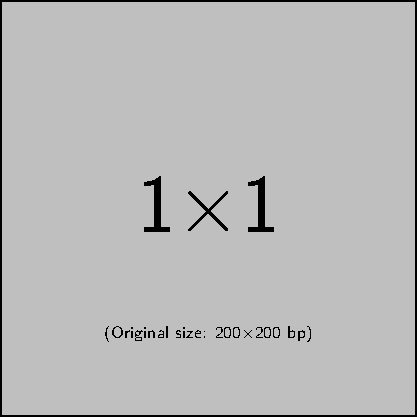
\includegraphics{example-image-1x1}%
      }%
    \end{captionbeside}
    \label{fig:maincls.captionbesidetop}
  \end{figure}
  \end{document}
\end{lstcode}
  \begin{figure}
    \KOMAoption{captions}{topbeside}
    \begin{captionbeside}[Beispiel: Bildbeschreibung daneben, oben]%
      {Eine Bildbeschreibung weder über noch unter der Abbildung,
        sondern oben daneben}[i][\linewidth]
      \raisebox{\dimexpr\baselineskip-\totalheight}{%
        \fbox{%
          \parbox[b][5\baselineskip][c]{.25\textwidth}{%
            \hspace*{\fill}\KOMAScript\hspace*{\fill}\par}}%
      }%
    \end{captionbeside}
    \label{fig:maincls.captionbesidetop}
  \end{figure}
\end{Example}
\vskip -1\ht\strutbox plus .75\strutbox% Beispiel am Ende der Erklärung
%
\EndIndexGroup


\begin{Declaration}
  \begin{Environment}{captionofbeside}
    \Parameter{Objekttyp}
    \OParameter{Verzeichnistitel}
    \Parameter{Titel}
    \OParameter{Anordnung}
    \OParameter{Breite}
    \OParameter{Offset}
    \begin{Body}\BodyDots\end{Body}
  \end{Environment}
  \labelsuffix[*]
  \begin{Environment}{captionofbeside}
    \Parameter{Objekttyp}
    \OParameter{Verzeichnistitel}
    \Parameter{Titel}
    \OParameter{Anordnung}
    \OParameter{Breite}
    \OParameter{Offset}\PValue{*}
    \begin{Body}\BodyDots\end{Body}
  \end{Environment}
\end{Declaration}
Wie\ChangedAt{v3.10}{\Class{scrbook}\and \Class{scrreprt}\and
  \Class{scrartcl}} zu \DescRef{\LabelBase.cmd.caption} mit
\DescRef{\LabelBase.cmd.captionof} eine Variante existiert, bei der der
\PName{Objekttyp} nicht durch die Verwendung innerhalb einer Gleitumgebung
dieses Typs bestimmt wird, so gibt es passend zur Umgebung
\DescRef{\LabelBase.env.captionbeside} mit \Environment{captionofbeside} auch
eine entsprechende Umgebung. Im Unterschied zu
\DescRef{\LabelBase.env.captionbeside} ist auch hier der \PName{Objekttyp} als
zusätzliches, erstes Argument anzugeben.%
%
\EndIndexGroup

\begin{Declaration}
  \FloatStyle{komaabove}
  \FloatStyle{komabelow}
\end{Declaration}%
Bei\OnlyAt{\Package{float}} Verwendung des
\Package{float}-Pakets\IndexPackage{float} wird das Aussehen der damit
definierten Gleitumgebungen allein vom \emph{float}-Stil bestimmt. Dies
schließt auch die Frage ein, ob mit Überschriften oder Unterschriften
gearbeitet wird. Im \Package{float}-Paket gibt es keinen vordefinierten Stil,
der im Aussehen dem von \KOMAScript{} entspricht und dieselben
Einstellmöglichkeiten (siehe unten) bietet. \KOMAScript{} definiert deshalb
zusätzlich die beiden Stile \PValue{komaabove} und \PValue{komabelow}. Diese
können bei Verwendung des \Package{float}-Pakets wie die dort definierten
Stile \PValue{plain}\IndexFloatstyle{plain},
\PValue{boxed}\IndexFloatstyle{boxed} oder
\PValue{ruled}\IndexFloatstyle{ruled} aktiviert werden. Siehe dazu
\cite{package:float}. Beim Stil \PValue{komaabove} werden \DescRef{\LabelBase.cmd.caption},
\DescRef{\LabelBase.cmd.captionabove} und \DescRef{\LabelBase.cmd.captionbelow} als Überschrift, beim Stil
\PValue{komabelow} als Unterschrift gesetzt.%
%
\EndIndexGroup


\begin{Declaration}
  \Macro{captionformat}
\end{Declaration}%
Bei {\KOMAScript} gibt es verschiedene Eingriffsmöglichkeiten, um die
Formatierung der Beschreibung zu ändern. Die Änderung der Schriftart
wurde bereits erläutert. Das oder die Trennzeichen zwischen dem Label
und dem eigentlichen Beschreibungstext sind im Makro
\Macro{captionformat} abgelegt.  Abweichend von allen anderen
\Macro{\dots}format-Anweisungen ist hier also nicht der Zähler,
sondern nur die auf den Zähler folgenden Angaben enthalten. Die
Originaldefinition lautet:
\begin{lstcode}
  \newcommand*{\captionformat}{:\ }
\end{lstcode}
Auch diese kann mit \Macro{renewcommand} geändert werden.
\begin{Example}
  Aus mir unerfindlichen Gründen wollen Sie als Trennzeichen
  keinen Doppelpunkt, gefolgt von einem Leerzeichen, sondern einen
  Gedankenstrich einschließlich der notwendigen Leerzeichen.
  Daher definieren Sie:
\begin{lstcode}
  \renewcommand*{\captionformat}{~--~}
\end{lstcode}
  Diese Definition sollten Sie beispielsweise in die Präambel Ihres
  Dokuments stellen.
\end{Example}
%
\EndIndexGroup
\vskip -1\ht\strutbox plus .75\ht\strutbox% Beispiel am Ende

\begin{Declaration}
  \Macro{figureformat}
  \Macro{tableformat}
\end{Declaration}%
Es wurde schon darauf hingewiesen, dass \DescRef{\LabelBase.cmd.captionformat}
keine Formatierung für das Label selbst enthält. Dieses sollte nun keineswegs
über Umdefinierung der Anweisungen für die Zählerausgabe, \Macro{thefigure}
oder \Macro{thetable}, verändert werden. Eine solche Umdefinierung hätte
nämlich auch Auswirkungen auf die Ausgabe von \Macro{ref} oder der
Verzeichnisse. Stattdessen bietet {\KOMAScript} zwei weitere \Macro{\dots
  format}-Anweisungen. Diese sind wie folgt vordefiniert:
\begin{lstcode}
  \newcommand*{\figureformat}{\figurename~\thefigure\autodot}
  \newcommand*{\tableformat}{\tablename~\thetable\autodot}
\end{lstcode}
\iffalse % Umbruchvarianten
Sie können ebenfalls mit \Macro{renewcommand} eigenen Anforderungen
angepasst werden.%
\else %
Mit \Macro{renewcommand} können diese leicht umdefiniert werden.%
\fi %
\begin{Example}
  Hin und wieder wird gewünscht, dass die Beschreibungstexte %
  \iffalse % Umbruchvarianten
  ganz ohne Label und natürlich auch ohne %
  \else %
  ohne Label und %
  \fi %
  Trennzeichen ausgegeben werden. Bei {\KOMAScript} genügen %
  \iffalse % Umbruchvarianten
  folgende Definitionen, um dies zu erreichen:%
  \else %
  dafür folgende Definitionen:%
  \fi %
\begin{lstcode}
  \renewcommand*{\figureformat}{}
  \renewcommand*{\tableformat}{}
  \renewcommand*{\captionformat}{}
\end{lstcode}
  Dabei ist jedoch zu beachten, dass die Nummerierung damit zwar nicht
  ausgegeben, aber dennoch fortgezählt wird. Dies ist insbesondere dann
  von Bedeutung, wenn die Umdefinierungen nur auf einzelne
  \Environment{figure}- oder \Environment{table}-Umgebungen angewendet
  werden.
\end{Example}
%
\EndIndexGroup
\vskip -1\ht\strutbox plus  .75\ht\strutbox% Beispiel am Ende der Erklärung

\begin{Declaration}
  \Macro{setcapindent}\Parameter{Einzug}
  \Macro{setcapindent*}\Parameter{Einzug}
  \Macro{setcaphanging}
\end{Declaration}%
Wie bereits erwähnt wurde, werden in den
Standardklassen\textnote{\KOMAScript{} vs. Standardklassen} die
Beschreibungen nicht hängend gesetzt. Das heißt: In mehrzeiligen
Beschreibungen beginnt die zweite Zeile direkt unter dem Labeltext.
Es gibt bei den Standardklassen auch keinen Mechanismus, dies direkt
zu beeinflussen. Bei {\KOMAScript} werden hingegen alle Zeilen ab der
zweiten so weit eingerückt, dass diese nicht mehr unter dem Label,
»Abbildung~\dots:« oder »Tabelle~\dots:«, sondern unter dem
eigentlichen Text der ersten Zeile beginnen.

Dieses Verhalten, das der Verwendung von \Macro{setcaphanging} entspricht,
kann bei {\KOMAScript} jederzeit durch \Macro{setcapindent} oder
\Macro{setcapindent*} geändert werden. Dabei gibt der Parameter \PName{Einzug}
an, wie weit ab der zweiten Zeile eingerückt werden soll.  Soll nach dem Label
und vor dem Beschreibungstext noch ein Zeilenumbruch erfolgen, so definieren
Sie die Einrücktiefe \PName{Einzug} der Beschreibung stattdessen mit der
Sternvariante der Anweisung: \Macro{setcapindent*}.  Mit einem negativen
\PName{Einzug} bei \Macro{setcapindent} erreicht man hingegen, dass vor der
Beschreibung ebenfalls ein Umbruch erfolgt und nur die erste Zeile der
Beschreibung, nicht jedoch die folgenden, um den Betrag von \PName{Einzug}
eingerückt werden.

Ob einzeilige Beschreibungen wie mehrzeilige Beschreibungen gesetzt werden
oder eine Sonderbehandlung erfahren, wird über die Option
\DescRef{\LabelBase.option.captions} gewählt. Siehe hierzu die Erklärung zu
den Werten \PValue{oneline} und \PValue{nooneline} dieser Option auf
\DescPageRef{\LabelBase.option.captions.oneline}.

\begin{Example}
  Die \hyperref[fig:maincls.caption.first]{%
    Abbildungen~\ref*{fig:maincls.caption.first}} bis
  \ref{fig:maincls.caption.last} zeigen die Auswirkungen unterschiedlicher
  Einstellungen. Es wird deutlich, dass bei geringer Spaltenbreite der
  komplett hängende Einzug unvorteilhaft ist. Der Quelltext der zweiten
  Abbildung sei hier mit gekürzter Unterschrift beispielhaft
  wiedergegeben:
\begin{lstcode}
  \begin{figure}
    \setcapindent{1em}
    \fbox{\parbox{.95\linewidth}{%
        \centering\KOMAScript}}
    \caption{Beispiel mit teilweise hängendem Einzug 
      ab der zweiten Zeile}
  \end{figure}
\end{lstcode}
  \begin{figure}
    \typeout{^^J--- Ignore underfull and overfull \string\hbox:}
    \addtokomafont{caption}{\small}
    \addtokomafont{captionlabel}{\bfseries}
    \centering%
    \begin{minipage}{.92\linewidth}
      \begin{minipage}[t]{.48\linewidth}\sloppy
        \fbox{\parbox{.95\linewidth}{\centering{\KOMAScript}}}
        \caption[Beispiel: Bildunterschrift mit Voreinstellung]%
        {Mit der Stan\-dard\-ein\-stel\-lung, also wie bei
          Verwendung von \Macro{setcaphanging}}
        \label{fig:maincls.caption.first}
      \end{minipage}
      \hspace{.02\linewidth}
      \begin{minipage}[t]{.48\linewidth}\sloppy
        \setcapindent{1em}
        \fbox{\parbox{.95\linewidth}{\centering{\KOMAScript}}}
        \caption[Beispiel: Bildunterschrift mit teilweise hängendem Einzug]%
        {Mit teilweise häng"-endem Einzug ab der zweiten Zeile durch
          Verwendung von \Macro{setcapindent}\PParameter{1em}}
      \end{minipage}
    \end{minipage}
    %\end{figure}
    \par\bigskip\noindent%
    %\begin{figure}
    %\addtokomafont{caption}{\small}
    %\addtokomafont{captionlabel}{\bfseries}
    %\centering
    \begin{minipage}{.9\linewidth}
      \begin{minipage}[t]{.48\linewidth}\sloppy
        \setcapindent*{1em}
        \fbox{\parbox{.95\linewidth}{\centering{\KOMAScript}}}
        \caption[Beispiel: Bildunterschrift mit hängendem Einzug und Umbruch]%
        {Mit hängendem Einzug ab der zweiten Zeile und Umbruch vor
          der Beschreibung durch Verwendung von
          \Macro{setcapindent*}\PParameter{1em}}
      \end{minipage}
      \hspace{.02\linewidth}
      \begin{minipage}[t]{.48\linewidth}\sloppy
        \setcapindent{-1em}
        \fbox{\parbox{.95\linewidth}{\centering{\KOMAScript}}}
        \caption[Beispiel: Bildunterschrift mit Einzug in der zweiten Zeile]%
        {Mit Einzug lediglich in der zweiten Zeile und einem Umbruch
          vor der Beschreibung durch Verwendung von
          \Macro{setcapindent}\PParameter{-1em}}
                \label{fig:maincls.caption.last}
      \end{minipage}
    \end{minipage}
    \typeout{^^J--- Don't ignore underfull and overfull
      \string\hbox:^^J}
  \end{figure}
\end{Example}
Wie im Beispiel zu sehen ist, kann die Formatierung auch lokal innerhalb einer
Gleitumgebung geändert werden. Die Änderung gilt dann nur für die eine
Umgebung. Nachfolgende Abbildungen und Tabellen werden wieder mit den
Grundeinstellungen oder den globalen Einstellungen, die Sie beispielsweise in
der Dokumentpräambel vorgenommen haben, gesetzt.%
\EndIndexGroup

\begin{Declaration}
  \Macro{setcapwidth}\OParameter{Ausrichtung}\Parameter{Breite}
  \Macro{setcapdynwidth}\OParameter{Ausrichtung}\Parameter{Breite}
  \Macro{setcapmargin}\OParameter{Rand \kern-.25em links}\Parameter{Rand}
  \Macro{setcapmargin*}\OParameter{Rand \kern-.25em innen}\Parameter{Rand}
\end{Declaration}
Mit\ChangedAt{v2.8q}{\Class{scrbook}\and \Class{scrreprt}\and
  \Class{scrartcl}} Hilfe dieser Befehle kann die Breite und Anordnung der
Beschreibung beeinflusst werden. Normalerweise steht die gesamte Text- oder
Spaltenbreite zur Verfügung.  Mit\important{\Macro{setcapwidth}} der Anweisung
\Macro{setcapwidth} kann diese \PName{Breite} reduziert werden. Dabei gibt das
obligatorische Argument die maximale für die Beschreibung verwendete
\PName{Breite} an. Als optionales Argument kann genau ein Buchstabe übergeben
werden, der die horizontale Ausrichtung der Beschreibung bestimmt. Die
möglichen Ausrichtungen finden Sie in der folgenden Liste.
\begin{labeling}[~--]{\quad\PValue{o}}\setlength{\itemsep}{-1\parsep plus 1ex}%
\item[\quad\PValue{l}] links
\item[\quad\PValue{r}] rechts
\item[\quad\PValue{i}] innen: auf rechten Seiten links, auf
  linken Seiten rechts
\item[\quad\PValue{o}] außen: auf rechten Seiten rechts, auf
  linken Seiten links
\end{labeling}
Die Ausrichtung innen und außen entspricht im einseitigen Satz linksbündig und
rechtsbündig. Innerhalb\textnote{Achtung!} von
\Package{longtable}\IndexPackage{longtable}-Tabellen%
\important{\Package{longtable}} funktioniert die Ausrichtung innen und außen
nicht korrekt. Insbesondere werden Beschreibungen von Folgeseiten bei diesen
Tabellen immer nach den Beschreibungen der ersten Teiltabelle
ausgerichtet. Dies ist ein konzeptionelles Problem des Pakets
\Package{longtable}.

Zu\ChangedAt{v3.20}{\Class{scrbook}\and \Class{scrreprt}\and
  \Class{scrartcl}}\textnote{Achtung!} beachten ist, dass die an
\Macro{setcapwidth} übergebene \PName{Breite} wie bei \Macro{setlength} zum
Zeitpunkt der Zuweisung ausgewertet
wird. Will\important{\Macro{setcapdynwidth}} man hingegen, dass \PName{Breite}
erst bei der Verwendung ausgewertet wird, kann man stattdessen
\Macro{setcapdynwidth} verwenden. Unterschiede gibt es beispielsweise, wenn
Längen wie \Length{linewidth} oder andere Anweisungen als Argument verwendet
werden.

Mit\important{\Macro{setcapmargin}} der Anweisung \Macro{setcapmargin} kann
statt der Breite der Beschreibung ein \PName{Rand} angegeben werden, der neben
der Beschreibung zusätzlich zum normalen Textrand eingehalten werden soll.
Sollen der Rand rechts und links nicht identisch gewählt werden, kann mit dem
optionalen Argument ein von \PName{Rand} abweichender \PName{Rand \kern-.25em
  links} von der Beschreibung eingestellt
werden. Bei\important{\Macro{setcapmargin*}} der Sternvariante
\Macro{setcapmargin*} wird statt \PName{Rand \kern-.25em links} im
doppelseitigen Satz \PName{Rand \kern-.25em innen} abweichend definiert.
Hier\textnote{Achtung!} ergibt sich bei
\Package{longtable}\IndexPackage{longtable}-Tabellen%
\important{\Package{longtable}} das gleiche Problem wie bei der Ausrichtung
außen oder innen bei der Anweisung \Macro{setcapwidth}. Die Verwendung von
\Macro{setcapmargin} oder \Macro{setcapmargin*} aktiviert außerdem
\OptionValueRef{\LabelBase}{captions}{nooneline} (siehe
\DescPageRef{\LabelBase.option.captions.nooneline}) für die Beschreibungen,
die mit dieser Randeinstellung gesetzt werden.

\iffalse% Umbruchkorrektur
Man\textnote{Tipp!} kann übrigens auch negative Werte für \PName{Rand} und
\PName{Rand \kern-.25em rechts} oder \PName{Rand \kern-.25em außen}
angeben. Dadurch erreicht man, dass die Beschreibung in den entsprechenden
Rand hineinragt.%
\else %
Soll\textnote{Tipp!} die Beschreibung in einen Rand ragen, gibt man übrigens
für das entsprechende Argument einfach einen negativen Wert an.%
\fi %
\iffalse\par% Anhang wurde entfernt.
Für\textnote{Tipp!} Experten und versierte Anwender ist eine etwas
trickreiche Anwendung für \Macro{setcapwidth} in
\iffree{\cite{book:komascript}}{\autoref{cha:floattricks},
  \autopageref{cha:floattricks}} zu finden.%
\fi%
%
\EndIndexGroup

\begin{Declaration}
  \Macro{setcaptionalignment}\OParameter{Gleitumgebung}\Parameter{Ausrichtung}
\end{Declaration}
Normalerweise\ChangedAt{v3.25}{\Class{scrbook}\and \Class{scrreprt}\and
  \Class{scrartcl}} werden mehrzeilige\textnote{Ausrichtung mehrzeiliger
  Beschreibungen} Beschreibungen im Blocksatz gesetzt. Dies entspricht
\Macro{setcaptionalignment}\PParameter{j}. Manchmal wird allerdings eine davon
abweichende Ausrichtung gewünscht, beispielsweise linksbündiger
Flattersatz. Eine entsprechende Änderung ist mit \Macro{setcaptionalignment}
jederzeit möglich. Für \PName{Ausrichtung} kann dabei genau einer der
Buchstaben aus \autoref{tab:maincls.captionalignment} angegeben werden. Wird
eine unbekannte \PName{Ausrichtung} angegeben, so resultiert dies in einer
Fehlermeldung.
%
\begin{table}
%  \centering
  \KOMAoptions{captions=topbeside}%
  \setcapindent{0pt}%
  \begin{captionbeside}
    [{Ausrichtungen für mehrzeilige Beschreibungen in Gleitumgebungen}]
    {\label{tab:maincls.captionalignment}%
      Ausrichtungen für mehrzeilige Beschreibungen in Gleitumgebungen}
    [l]
    \begin{tabular}[t]{ll}
      \toprule
      c & zentriert \\
      j & Blocksatz \\
      l & linksbündig \\
      r & rechtsbündig \\
      C & zentriert mit \Package{ragged2e} \\
      J & Blocksatz mit \Package{ragged2e} \\
      L & linksbündig mit \Package{ragged2e} \\
      R & rechtsbündig mit \Package{ragged2e} \\
      \bottomrule
    \end{tabular}
  \end{captionbeside}
\end{table}

Die vier Möglichkeiten mit Paket
\Package{ragged2e}\important{\Package{ragged2e}}\IndexPackage{ragged2e} stehen
nur zur Verfügung, wenn das Paket vor Verwendung von
\Macro{setcaptionalignment} geladen wurde. Anderenfalls werden sie auf die
entsprechenden Möglichkeiten ohne \Package{ragged2e} abgebildet. Zur
Sicherheit wird in diesem Fall eine Warnung ausgegeben.

Verwendet man den Befehl ohne\textnote{kein optionaler Parameter} den
optionalen Parameter, so hängt das Ergebnis davon ab, ob der Aufruf innerhalb
oder außerhalb einer Gleitumgebung stattfindet. Innerhalb einer Gleitumgebung
wird dann die Ausrichtung für diese Gleitumgebung gesetzt. Außerhalb wird
hingegen ein leerer optionaler Parameter angenommen.

Beim Aufruf mit einem leeren\textnote{leerer optionaler Parameter} optionalen
Parameter oder außerhalb einer Gleitumgebung auch komplett ohne optionalen
Parameter wird die allgemeine Ausrichtung festgelegt. Diese wird immer dann
verwendet, wenn keine Ausrichtung für den aktuellen Gleitumgebungstyp
definiert ist.

Will man nur die Ausrichtung eines bestimmen Typs\textnote{mit
  \PName{Gleitumgebung}} von Gleitumgebungen festlegen, ohne
\PName{Ausrichtung} auch für andere Arten von Gleitumgebungen zu verändern, so
gibt man den Typ der Gleitumgebung, beispielsweise \PValue{figure} oder
\PValue{table}, als optionalen Parameter \PName{Gleitumgebung} an.
%
\begin{Example}
  Sie wollen, dass Bildunterschriften auch dann vollständig zentriert unter
  den Bildern stehen, wenn sie mehrzeilig sind. Um das zunächst einmal nur für
  eine einzige Abbildung zu testen, verwenden Sie\textnote{in der
    Gleitumgebung}:
\begin{lstcode}
  \begin{figure}
    \centering
    \setcaptionalignment{c}
    
\includegraphics{example-image}
    \caption{\blindtext}
  \end{figure}
\end{lstcode}
  Da Sie mit dem Ergebnis zufrieden sind, verschieben Sie die
  Anweisung\textnote{in der Dokumentpräambel}
\begin{lstcode}
  \setcaptionalignment{c}
\end{lstcode}
  in die Dokumentpräambel. Daraufhin bemerken Sie allerdings, dass Ihnen
  diese Änderung für Tabellenüberschriften überhaupt nicht gefällt. Daher
  beschränken Sie mit\textnote{nur für Abbildungen}
\begin{lstcode}
  \setcaptionalignment[figure]{c}
\end{lstcode}
  die Zentrierung auf Abbildungen.

  Etwas später stellen Sie fest, dass die Zentrierung doch nicht so günstig
  ist. Stattdessen wollen Sie nun lieber eine linksbündige Ausrichtung im
  Flattersatz haben. Also ändern Sie die Anweisung erneut zu:
\begin{lstcode}
  \setcaptionalignment[figure]{l}
\end{lstcode}
  Allerdings gefällt Ihnen nun nicht, dass die Zeilen sehr unterschiedlich
  lang werden. Als Ursache machen Sie die fehlende Trennung aus, wodurch lange
  Wörter komplett in die nächste Zeile rutschen und so große Lücken
  hinterlassen. Also wollen Sie zusätzlich Trennung nach Bedarf
  ermöglichen. Dies ist mit Hilfe des Pakets
  \Package{ragged2e}\important{\Package{ragged2e}}\IndexPackage{ragged2e}
  leicht möglich. Dabei genügt es allerdings nicht, das Paket mit
\begin{lstcode}
  \usepackage{ragged2e}
\end{lstcode}
  zu laden. Auch Option \Option{newcommands} beim Laden des Pakets bringt
  keine Abhilfe. Stattdessen muss zusätzlich die \PName{Ausrichtung} geändert
  werden:
\begin{lstcode}
  \usepackage{ragged2e}
  \setcaptionalignment[figure]{L}
\end{lstcode}
  Beachten\textnote{Achtung!} Sie den Großbuchstabe für \PName{Ausrichtung}.
\end{Example}
\EndIndexGroup


\begin{Declaration}
  \Option{origlongtable}
\end{Declaration}%
\BeginIndex{Package}{longtable}%
Falls die Tabellenüberschriften des \Package{longtable}-Pakets (siehe
\cite{package:longtable}) von den \KOMAScript-Klassen nicht umdefiniert werden
sollen, kann die Option \Option{origlongtable} %
\iffalse % Umbruchkorrektur
gesetzt werden. Diese Option\textnote{Achtung!}  ist als optionales Argument
von \DescRef{\LabelBase.cmd.documentclass} zu verwenden. %
\else %
beim Laden der Klasse gesetzt werden. \textnote{Achtung!}%
\fi %
Eine Einstellung per \DescRef{\LabelBase.cmd.KOMAoptions} oder
\DescRef{\LabelBase.cmd.KOMAoption} wird nicht unterstützt.
%
\EndIndexGroup
%
\EndIndexGroup


\begin{Declaration}
  \OptionVName{listof}{Einstellung}
\end{Declaration}
Normalerweise\ChangedAt{v3.00}{\Class{scrbook}\and \Class{scrreprt}\and
  \Class{scrartcl}} werden Verzeichnisse von Gleitumgebungen --~wie das
Tabellen"~\Index{Tabellen>Verzeichnis} und das
Abbildungsverzeichnis\Index{Abbildungen>Verzeichnis}~-- nicht nummeriert oder
in das Inhaltsverzeichnis aufgenommen. In \autoref{sec:\LabelBase.toc} wurde
dies bereits näher ausgeführt. Alternativ zu den dort erwähnten Einstellungen
\OptionValueRef{\LabelBase}{toc}{nolistof}%
\IndexOption{toc~=\textKValue{nolistof}},
\OptionValueRef{\LabelBase}{toc}{listof}\IndexOption{toc~=\textKValue{listof}}
und \OptionValueRef{\LabelBase}{toc}{listofnumbered}%
\IndexOption{toc~=\textKValue{listofnumbered}}, kann dieses Verhalten auch aus
Sicht der Verzeichnisse selbst gesehen werden. Daher kann man die gleichen
Ergebnisse auch mit den Einstellungen \OptionValue{listof}{notoc},
\OptionValue{listof}{totoc} und \OptionValue{listof}{numbered} erreichen.

Dabei wird in der Voreinstellung für die Überschriften der Verzeichnisse die
oberste verfügbare Gliederungsebene unterhalb von
\DescRef{\LabelBase.cmd.part} verwendet. Bei \Class{scrbook} und
\Class{scrreprt} ist das die Kapitelebene, bei \Class{scrartcl} die
Abschnittsebene. Mit\important{\OptionValue{listof}{leveldown}}%
\ChangedAt{v3.06}{\Class{scrbook}\and \Class{scrreprt}\and \Class{scrartcl}}
Hilfe der Einstellung \OptionValue{listof}{leveldown} kann hingegen die
nächsttiefere Gliederungsebene verwendet
werden. \important{\OptionValue{listof}{standardlevel}}%
\ChangedAt{v3.15}{\Class{scrbook}\and \Class{scrreprt}\and \Class{scrartcl}}%
\OptionValue{listof}{standardlevel} schaltet bei Bedarf wieder zurück auf die
voreingestellte Gliederungsebene.
\begin{Example}
  Sie wollen in einem Buch das Abbildungs- und das Tabellenverzeichnis als
  Unterverzeichnisse eines gemeinsamen Verzeichnisses »Abbildungen und
  Tabellen« setzen. Dazu verwenden Sie einfach:
\begin{lstcode}
  \KOMAoption{listof}{leveldown}
\end{lstcode}
  und dann an entsprechender Stelle Ihres Dokuments:
\begin{lstcode}
  \addchap*{Abbildungs- und Tabellenverzeichnis}
  \listoffigures
  \listoftables
\end{lstcode}
  Näheres zur Anweisung \DescRef{\LabelBase.cmd.addchap*} ist
  \autoref{sec:\LabelBase.structure}, \DescPageRef{\LabelBase.cmd.addchap*} zu
  entnehmen.
\end{Example}

Normalerweise\ChangedAt{v2.8q}{%
  \Class{scrbook}\and \Class{scrreprt}\and \Class{scrartcl}} werden die
Verzeichnisse\Index{Abbildungen>Verzeichnis}\Index{Tabellen>Verzeichnis}
der Gleitumgebungen so formatiert, dass für die Nummer ein Raum fester Breite
verwendet wird. Gleichzeitig werden alle Einträge leicht eingezogen. Dies
entspricht der Verwendung der Einstellung
\OptionValue{listof}{graduated}\IndexOption{listof~=\textKValue{graduated}}.

Werden die Nummern sehr breit, weil beispielsweise sehr viele Tabellen
verwendet werden, so reicht der vorgesehene Platz irgendwann nicht mehr aus.
Vergleichbar\important{\OptionValue{listof}{flat}} zur Einstellung
\OptionValueRef{\LabelBase}{toc}{flat}\IndexOption{toc~=\textKValue{flat}} für
das Inhaltsverzeichnis bietet \KOMAScript{} daher die Einstellung
\OptionValue{listof}{flat}\IndexOption{listof~=\textKValue{flat}} für die
Verzeichnisse der Gleitumgebungen. Dabei wird die Breite der Nummern
automatisch ermittelt und der Platz entsprechend angepasst. Bezüglich der
Nebenwirkungen und Funktionsweise gilt, was in \autoref{sec:\LabelBase.toc},
\DescPageRef{\LabelBase.option.toc.flat} für die Einstellung
\OptionValueRef{\LabelBase}{toc}{flat} erklärt wurde. Es sei an dieser Stelle
jedoch nochmals darauf hingewiesen, dass mit der Einstellung
\OptionValue{listof}{flat} mehrere \LaTeX-Durchläufe benötigt werden, bis die
Verzeichnisse ihre endgültige Form erhalten haben.

Die Einstellung \OptionValue{listof}{flat} wird automatisch aktiviert, falls
die Einstellung
\OptionValue{listof}{entryprefix}\ChangedAt{v3.06}{\Class{scrbook}\and
  \Class{scrreprt}\and \Class{scrartcl}} verwendet
wird. Normalerweise\important{\OptionValue{listof}{entryprefix}} ist es nicht
sinnvoll jeden Eintrag in eines der Verzeichnisse der Gleitumgebungen mit
einem Präfix wie »Abbildung« oder »Tabelle« zu versehen, da natürlich im
Abbildungsverzeichnis nur Abbildungen und im Tabellenverzeichnis nur Tabellen
zu finden sind. Damit hat ein solcher Präfix keinen zusätzlichen
Informationswert und wird in der Voreinstellung auch weggelassen. Mit der
Einstellung \OptionValue{listof}{entryprefix} wird ein solcher Präfix jedoch
gesetzt. Dabei erhalten alle Einträge eines Verzeichnisses denselben
Präfix. Dieser richtet sich nach dem Dateianhang der Hilfsdatei, die für das
Verzeichnis verwendet wird. Für das Abbildungsverzeichnis, das den Dateianhang
»\File{lof}« besitzt, wird beispielsweise \Macro{listoflofentryname} verwendet,
während für das Tabellenverzeichnis, das den Dateianhang »\File{lot}« besitzt,
\Macro{listoflotentryname} verwendet wird.

Bei den Klassen \Class{scrbook} und
\Class{scrreprt}\OnlyAt{\Class{scrbook}\and \Class{scrreprt}} fügt
\KOMAScript{} in der Voreinstellung bei jedem Kapitelanfang einen vertikalen
Abstand in die Verzeichnisse der Gleitumgebungen ein. Dieses Verhalten, das es
auch bei den Standardklassen gibt, dient dazu, diese Verzeichnisse nach
Kapiteln zu gruppieren. Es entspricht bei \KOMAScript{} der
Einstellung\ChangedAt{v3.00}{\Class{scrbook}\and \Class{scrreprt}\and
  \Class{scrartcl}} \OptionValue{listof}{chaptergapsmall}%
\LabelOptionValue{listof}{chaptergapsmall}%
\important{\OptionValue{listof}{chaptergapsmall}}%
\IndexOption{listof~=\textKValue{chaptergapsmall}}.  Dabei wird ein fester
vertikaler Abstand von 10\Unit{pt}
verwendet. Mit\important{\OptionValue{listof}{chaptergapline}} der Einstellung
\OptionValue{listof}{chaptergapline}%
\IndexOption{listof~=\textKValue{chaptergapline}} kann man stattdessen einen
vertikalen Abstand von einer Zeile
erreichen. Mit\important{\OptionValue{listof}{nochaptergap}}
\OptionValue{listof}{nochaptergap}%
\IndexOption{listof~=\textKValue{nochaptergap}} kann man den vertikalen
Abstand komplett
abschalten. Eine\important{\OptionValue{listof}{chapterentry}} Besonderheit
stellt die Einstellung \OptionValue{listof}{chapterentry}%
\IndexOption{listof~=\textKValue{chapterentry}} dar. Dabei wird statt des
Abstandes der Inhaltsverzeichniseintrag für das Kapitel in das Verzeichnis der
Gleitumgebungen eingefügt. Es\textnote{Achtung!} wird darauf hingewiesen, dass
ein solcher Eintrag auch dann erfolgt, wenn das Kapitel keine Gleitumgebung
enthält. Eine Lösung, bei der nur Kapitel mit Gleitumgebungen im jeweiligen
Verzeichnis angezeigt werden, finden Sie unter
\cite{https://komascript.de/comment/5070}. Eine noch direktere Beeinflussung,
was in den Verzeichnissen der Gleitumgebungen bei neuen Kapiteln geschehen
soll, ist mit der Option \DescRef{\LabelBase.option.chapteratlists} zu
erreichen, die in \autoref{sec:\LabelBase.structure} auf
\DescPageRef{\LabelBase.option.chapteratlists} erläutert wird.

Ein Überblick über alle möglichen Werte für die \PName{Einstellung} von
\Option{listof} ist in \autoref{tab:maincls.listof} zu finden.

\begin{desclist}
  \desccaption[{Mögliche Werte für Option \Option{listof}}]{%
    Mögliche Werte für Option \Option{listof} zur Einstellung von Form und
    Inhalt der Verzeichnisse der Gleitumgebungen\label{tab:maincls.listof}%
  }{%
    Mögliche Werte für Option \Option{listof} (\emph{Fortsetzung})%
  }%
  \entry{\PValue{chapterentry}, \PValue{withchapterentry}}{%
    Kapitelanfänge werden in den Verzeichnissen der Gleitumgebungen durch
    einen Inhaltsverzeichniseintrag des Kapitels markiert.%
    \IndexOption{listof~=\textKValue{chapterentry}}}%
  \entry{\PValue{chaptergapline}, \PValue{onelinechaptergap}}{%
    Kapitelanfänge werden in den Verzeichnissen der Gleitumgebungen durch
    einen Abstand von einer Zeile markiert.%
    \IndexOption{listof~=\textKValue{chaptergapline}}}%
  \entry{\PValue{chaptergapsmall}, \PValue{smallchaptergap}}{%
    Kapitelanfänge werden in den Verzeichnissen der Gleitumgebungen durch
    einen kleinen Abstand markiert.%
    \IndexOption{listof~=\textKValue{chaptergapsmall}}}%
  \entry{\PValue{entryprefix}}{%
    \ChangedAt{v3.06}{\Class{scrbook}\and \Class{scrreprt}\and
      \Class{scrartcl}}%
    Jeder Verzeichniseintrag wird mit einem vom Verzeichnis abhängenden Präfix
    vor der Nummer versehen. Der Präfix ist normalerweise sprachabhängig,
    beispielsweise bei deutschen Spracheinstellungen »Abbildung« für das
    Abbildungsverzeichnis und »Tabelle« für das Tabellenverzeichnis, jeweils
    gefolgt von einem Leerzeichen.%
    \IndexOption{listof~=\textKValue{entryprefix}}}%
  \entry{\PValue{flat}, \PValue{left}}{%
    Die Verzeichnisse der Gleitumgebungen erhalten eine tabellarische
    Form. Die Gleitumgebungsnummern sind dabei die erste Spalte, der Titel die
    zweite Spalte, die Seitenzahlen die dritte Spalte. Der Platz, der für die
    Gleitumgebungsnummern reserviert wird, richtet sich nach dem benötigten
    Platz des vorherigen \LaTeX-Laufs.%
    \IndexOption{listof~=\textKValue{flat}}}%
  \entry{\PValue{graduated}, \PValue{indent}, \PValue{indented}}{%
    Die Verzeichnisse der Gleitumgebungen erhalten eine hierarchische Form. Es
    steht nur ein begrenzter Platz für die Gleitumgebungsnummern zur
    Verfügung.%
    \IndexOption{listof~=\textKValue{graduated}}}%
  \entry{\PValue{indenttextentries}, \PValue{indentunnumbered},
    \PValue{numberline}}{%
    \ChangedAt{v3.12}{\Class{scrbook}\and \Class{scrreprt}\and
      \Class{scrartcl}}%
    Die Eigenschaft \PValue{numberline} (siehe \autoref{sec:tocbasic.toc},
    \DescPageRef{tocbasic.cmd.setuptoc}) wird für die Verzeichnisse der
    Gleitumgebungen, beispielsweise das Abbildungs"~ und das
    Tabellenverzeichnis, gesetzt. Dadurch werden nicht nummerierte Einträge
    linksbündig mit dem Text von nummerierten Einträgen gleicher Ebene
    gesetzt. Allerdings bieten die \KOMAScript-Klassen selbst keine nicht
    nummerierten Einträge in diese Verzeichnisse. Dies hat daher nur
    Auswirkungen auf entsprechende Einträge, die nicht von den Klassen selbst,
    aber dennoch mit Hilfe von \DescRef{tocbasic.cmd.addxcontentsline} (siehe
    \autoref{sec:tocbasic.toc}, \DescPageRef{tocbasic.cmd.addxcontentsline})
    erzeugt werden.%
    \IndexOption{toc~=\textKValue{numberline}}}%
  \entry{\PValue{leftaligntextentries}, \PValue{leftalignunnumbered},
    \PValue{nonumberline}}{%
    \ChangedAt{v3.12}{\Class{scrbook}\and \Class{scrreprt}\and
      \Class{scrartcl}}%
    Die Eigenschaft \PValue{numberline} (siehe \autoref{sec:tocbasic.toc},
    \DescPageRef{tocbasic.cmd.setuptoc}) wird für die Verzeichnisse der
    Gleitumgebungen, beispielsweise das Abbildungs"~ und das
    Tabellenverzeichnis, gelöscht. Dadurch werden nicht nummerierte Einträge
    linksbündig mit der Nummer von nummerierten Einträgen gleicher Ebene
    gesetzt. Allerdings bieten die \KOMAScript-Klassen selbst keine nicht
    nummerierten Einträge in diese Verzeichnisse. Dies hat daher nur
    Auswirkungen auf entsprechende Einträge, die nicht von den Klassen selbst,
    aber dennoch mit Hilfe von \DescRef{tocbasic.cmd.addxcontentsline} (siehe
    \autoref{sec:tocbasic.toc}, \DescPageRef{tocbasic.cmd.addxcontentsline})
    erzeugt werden.%
    \IndexOption{toc~=\textKValue{numberline}}}%
  \entry{\PValue{leveldown}}{%
    Die Verzeichnisse werden um eine Gliederungsebene nach unten verschoben.%
    \IndexOption{listof~=\textKValue{leveldown}}}%
  \entry{\PValue{nochaptergap}, \PValue{ignorechapter}}{%
    Kapitelanfänge werden in den Verzeichnissen der Gleitumgebungen nicht
    markiert.%
    \IndexOption{listof~=\textKValue{nochaptergap}}}%
  \entry{\PValue{notoc}, \PValue{nottotoc}, \PValue{plainheading}}{%
    Die Verzeichnisse der Gleitumgebungen, beispielsweise das Abbildungs"~ und
    das Tabellenverzeichnis, erhalten keinen Eintrag im Inhaltsverzeichnis.%
    \IndexOption{listof~=\textKValue{nottotoc}}}%
  \entry{\PValue{numbered}, \PValue{totocnumbered}, \PValue{tocnumbered},
    \PValue{numberedtoc}, \PValue{numberedtotoc}}{%
    Die Verzeichnisse der Gleitumgebungen, beispielsweise das Abbildungs"~ und
    das Tabellenverzeichnis, erhalten einen Eintrag im Inhaltsverzeichnis und
    werden nummeriert.%
    \IndexOption{listof~=\textKValue{numbered}}}%
  \entry{\PValue{standardlevel}}{%
    Die Verzeichnisse liegen auf der üblichen Gliederungsebene.%
    \IndexOption{listof~=\textKValue{standardlevel}}}%
  \entry{\PValue{toc}, \PValue{totoc}, \PValue{notnumbered}}{%
    Die Verzeichnisse der Gleitumgebungen, beispielsweise das Abbildungs"~ und
    das Tabellenverzeichnis, erhalten einen Eintrag im Inhaltsverzeichnis,
    ohne dass sie nummeriert werden.%
    \IndexOption{listof~=\textKValue{totoc}}}%
\end{desclist}
%
\EndIndexGroup


\begin{Declaration}
  \Macro{listoftables}
  \Macro{listoffigures}
\end{Declaration}%
Mit diesen Anweisungen kann ein Verzeichnis der Tabellen beziehungsweise der
Abbildungen ausgegeben werden. Änderungen, die Auswirkungen auf diese
Verzeichnisse haben, werden erst nach zwei \LaTeX{}-Läufen sichtbar. Die Form
der Verzeichnisse kann durch die Option
\DescRef{\LabelBase.option.listof}\important{\DescRef{\LabelBase.option.listof}}
mit den Werten \PValue{graduated} und \PValue{flat} beeinflusst werden (siehe
\DescPageRef{\LabelBase.option.listof}). Darüber hinaus wirken sich indirekt
die Werte \PValue{listof} und \PValue{listofnumbered} für die Option
\DescRef{\LabelBase.option.toc}\important{\DescRef{\LabelBase.option.toc}}
(siehe \autoref{sec:\LabelBase.toc}, \DescPageRef{\LabelBase.option.toc})
sowie die Werte \PValue{totoc} und \PValue{numbered} der oben erläuterten
Option \DescRef{\LabelBase.option.listof} auf die Verzeichnisse aus.

In\textnote{Tipp!} der Regel findet man die Verzeichnisse der
Gleitumgebungen\Index{Gleitumgebungen}, also das 
\index{Tabellen>Verzeichnis}Tabellen- und das 
Abbildungsverzeichnis\index{Abbildungen>Verzeichnis}, unmittelbar nach dem
Inhaltsverzeichnis. In einigen Dokumenten wandern diese auch in den
Anhang. Der Autor bevorzugt jedoch die Platzierung unmittelbar nach dem
Inhaltsverzeichnis.%
%
\EndIndexGroup


\LoadCommonFile{marginpar}% \section{Randnotizen}


\section{Anhang}
\seclabel{appendix}
\BeginIndexGroup
\BeginIndex{}{Anhang}

Der Anhang eines Dokuments besteht im Wesentlichen aus den Anlagen zu einem
Dokument. Typische Teile eines Anhangs sind Literaturverzeichnis,
Stichwortverzeichnis und Begriffsverzeichnis. Alleine für diese Teile würde
man jedoch keinen Anhang beginnen, da diese Teile normalerweise schon von sich
aus eine Auszeichnung besitzen, die sie als Anhang erkennbar macht. Enthält
der Anhang aber weitere Teile wie beispielsweise zitierte Fremddokumente,
Endnoten oder Tafeln, so werden die zuvor genannten Teile ebenfalls im Anhang
gesetzt.


\begin{Declaration}
  \Macro{appendix}
\end{Declaration}%
Der Anhang wird in den Standardklassen und den {\KOMAScript}-Klassen mit der
Anweisung \Macro{appendix} eingeleitet. Diese Anweisung schaltet unter anderem
die Kapitelnummerierung auf Großbuchstaben um und sorgt gleichzeitig dafür,
dass die Regeln für die Nummerierung der Gliederungsebenen nach \cite{DUDEN}
eingehalten werden. Diese Regeln sind in der Beschreibung der Option
\DescRef{\LabelBase.option.numbers} in \autoref{sec:\LabelBase.structure},
\DescPageRef{\LabelBase.option.numbers} näher erläutert.

Die Form der Kapitelüberschriften\OnlyAt{\Class{scrbook}\and \Class{scrreprt}}
im Anhang wird durch die Optionen \DescRef{\LabelBase.option.chapterprefix}%
\important{\DescRef{\LabelBase.option.chapterprefix}\\
  \DescRef{\LabelBase.option.appendixprefix}} und
\DescRef{\LabelBase.option.appendixprefix} bestimmt. Näheres dazu ist
\autoref{sec:\LabelBase.structure},
\DescPageRef{\LabelBase.option.appendixprefix} zu entnehmen.

Bitte\textnote{Achtung!} beachten Sie, dass es sich bei \Macro{appendix} um
eine Anweisung und \emph{nicht} um eine Umgebung handelt! Die Anweisung
erwartet auch nicht etwa ein Argument. Die Kapitel beziehungsweise Abschnitte
des Anhangs werden ganz normal mit \DescRef{\LabelBase.cmd.chapter} und
\DescRef{\LabelBase.cmd.section} gesetzt.%
%
\EndIndexGroup
%
\EndIndexGroup


\section{Literaturverzeichnis}
\seclabel{bibliography}
\BeginIndexGroup
\BeginIndex{}{Literaturverzeichnis}

Das Literaturverzeichnis erschließt externe Quellen. In der Regel wird das
Literaturverzeichnis mit Hilfe des Programms \BibTeX{} aus einer Datei mit
datenbankähnlicher Struktur erzeugt. Dabei kann über den \BibTeX-Stil sowohl
die Form der Einträge als auch deren Sortierung verändert werden. Wird
zusätzlich ein Literaturpaket, beispielsweise
\Package{natbib}\IndexPackage{natbib},
\Package{babelbib}\IndexPackage{babelbib} oder
\Package{biblatex}\IndexPackage{biblatex} verwendet, so schwindet der Einfluss
von \KOMAScript{} auf das Literaturverzeichnis. In diesen Fällen ist unbedingt
die Anleitung des verwendeten Pakets zu beachten! Zur generellen Verwendung
eines Literaturverzeichnisses sei auf \cite{l2kurz} verwiesen.


\begin{Declaration}
  \OptionVName{bibliography}{Einstellung}
\end{Declaration}
Als \PName{Einstellung}\ChangedAt{v3.00}{\Class{scrbook}\and
  \Class{scrreprt}\and \Class{scrartcl}} kann zunächst einmal jeder definierte
Formatierungsstil gewählt werden. Vordefiniert sind bei \KOMAScript{} zwei
solche Formatierungsstile für das Literaturverzeichnis. Diese sind jedoch
nicht zu verwechseln mit den unterschiedlichen Stilen für
\BibTeX\Index{BibTeX=\BibTeX}, die man mit \Macro{bibstyle} auswählt. Während
\BibTeX{} sowohl die Art der Sortierung als auch den Inhalt des
Literaturverzeichnisses bestimmt, können über die Einstellungen von
\KOMAScript{} nur grundlegende Eigenschaften des Literaturverzeichnisses oder
einige wenige Eigenschaften der Formatierung der Einträge beeinflusst werden.

Mit\important{\OptionValue{bibliography}{oldstyle}}
\OptionValue{bibliography}{oldstyle}%
\IndexOption{bibliography~=\textKValue{oldstyle}} wird die kompakte Formatierung
gewählt. Dabei führt die Anweisung
\DescRef{maincls-experts.cmd.newblock}\IndexCmd{newblock} in den einzelnen
Einträgen lediglich zu einem dehnbaren horizontalen Abstand. Der Name kommt
daher, dass dies die häufigste klassische Form eines Literaturverzeichnisses
ist. Demgegenüber\important{\OptionValue{bibliography}{openstyle}} erreicht
man die etwas modernere, offene Form mit der Einstellung
\OptionValue{bibliography}{openstyle}%
\IndexOption{bibliography~=\textKValue{openstyle}}. Der Name kommt daher, dass
hier die Anweisung \DescRef{maincls-experts.cmd.newblock} einen Absatz
einfügt. Die Einträge im Literaturverzeichnis werden so stärker
gegliedert. Sie sind weniger kompakt und deutlich aufgelockerter oder
geöffnet.  Bezüglich der Möglichkeit, neue Formatierungsstile zu definieren,
sei auf \DescRef{maincls-experts.cmd.newbibstyle},
\autoref{sec:maincls-experts.bibliography},
\DescPageRef{maincls-experts.cmd.newbibstyle} verwiesen.

Neben dem Formatierungsstil gibt es eine weitere Eigenschaft, die über
\PName{Einstellung} verändert werden kann. Das Literaturverzeichnis stellt
eine Art von Verzeichnis dar, bei der nicht der Inhalt des vorliegenden Werks
aufgelistet, sondern auf externe Inhalte verwiesen wird. Mit dieser Begründung
könnte man argumentieren, dass das Literaturverzeichnis ein eigenes Kapitel
bzw. einen eigenen Abschnitt darstellt und somit eine Nummer verdiene.  Die
Einstellung \OptionValue{bibliography}{numbered}%
\important{\OptionValue{bibliography}{numbered}}%
\IndexOption{bibliography~=\textKValue{numbered}} führt genau dazu,
einschließlich des dann fälligen Eintrags im Inhaltsverzeichnis.  Ich selbst
bin der Meinung, dass bei dieser Argumentation auch ein klassisches,
kommentiertes Quellenverzeichnis ein eigenes Kapitel wäre. Außerdem ist das
Literaturverzeichnis letztlich nichts, was man selbst geschrieben
hat. Deshalb\important{\OptionValue{bibliography}{totoc}} verdient es
allenfalls einen nicht nummerierten Eintrag im Inhaltsverzeichnis, was mit der
Einstellung
\OptionValue{bibliography}{totoc}\IndexOption{bibliography~=\textKValue{totoc}}
erreicht wird. Die Voreinstellung, bei der das Literaturverzeichnis als nicht
nummeriertes Kapitel\important{\OptionValue{bibliography}{nottotoc}}%
\IndexOption{bibliography~=\textKValue{nottotoc}} ohne eigenen
Inhaltsverzeichniseintrag gesetzt wird, entspricht
\OptionValue{bibliography}{nottotoc}. Siehe hierzu auch Option
\DescRef{\LabelBase.option.toc} in \autoref{sec:\LabelBase.toc}, insbesondere
die Werte \PValue{bibliographynumbered}, \PValue{bibliography} und
\PValue{nobibliography} ab \DescPageRef{\LabelBase.option.toc.bibliography}.

In\ChangedAt{v3.12}{\Class{scrbook}\and \Class{scrreprt}\and \Class{scrartcl}}
einigen Fällen wird nicht das gesamte Dokument mit einem einzigen
Literaturverzeichnis versehen, sondern jedes Kapitel eines mit \Class{scrbook}
oder \Class{scrreprt} gesetzten Dokuments erhält sein eigenes
Literaturverzeichnis. In diesem Fall ist es sinnvoll,
wenn\important{\OptionValue{bibliography}{leveldown}} das Literaturverzeichnis
selbst nicht auf Kapitelebene, sondern etwas tiefer auf Abschnittsebene
angesiedelt wird. Dies ist mit Option \OptionValue{bibliography}{leveldown}%
\IndexOption{bibliography~=\textKValue{leveldown}} zu erreichen. Die
Einstellung kann auch verwendet werden, wenn das Literaturverzeichnis zusammen
mit anderen Verzeichnissen unter einer gemeinsamen Überschrift erscheinen
soll. Daher ist diese Option auch in \Class{scrartcl} verfügbar.

Eine Zusammenfassung möglicher Werte für \PName{Einstellung} ist
\autoref{tab:maincls.bibliography} zu entnehmen. Es ist jedoch zu beachten,
dass mit \DescRef{maincls-experts.cmd.newbibstyle}\IndexCmd{newbibstyle}
weitere Werte definiert werden können.

\begin{table}
  \caption[{Mögliche Werte für Option \Option{bibliography}}]{Vordefinierte
    Werte für Option \Option{bibliography} zur Einstellung der Form des
    Literatur\-verzeichnisses}
  \label{tab:maincls.bibliography}
  \begin{desctabular}
    \pventry{leveldown}{%
      \ChangedAt{v3.12}{\Class{scrbook}\and \Class{scrreprt}\and
        \Class{scrartcl}}%
      Das Literaturverzeichnis wird um eine Gliederungsebene nach unten
      verschoben.%
      \IndexOption{bibliography~=\textKValue{leveldown}}}\\[-1.7ex]
    \entry{\PValue{notoc}, \PValue{nottotoc}, \PValue{plainheading}}{%
      Das Literaturverzeichnis erhält keinen Eintrag im Inhaltsverzeichnis und
      wird auch nicht nummeriert.%
      \IndexOption{bibliography~=\textKValue{nottotoc}}}\\[-1.7ex]
    \entry{\PValue{numbered}, \PValue{tocnumbered}, \PValue{totocnumbered},
      \PValue{numberedtoc}, \PValue{numberedtotoc}}{%
      Das Literaturverzeichnis erhält einen Eintrag im Inhaltsverzeichnis und
      wird nummeriert.%
      \IndexOption{bibliography~=\textKValue{numbered}}}\\[-1.7ex]
    \pventry{oldstyle}{%
      Es wird die klassische, kompakte Formatierung gewählt, bei der
      \DescRef{maincls-experts.cmd.newblock}\IndexCmd{newblock} nur einen
      dehnbaren horizontalen Abstand darstellt.%
      \IndexOption{bibliography~=\textKValue{oldstyle}}}\\[-1.7ex]
    \pventry{openstyle}{%
      Es wird eine untergliederte, offene Formatierung gewählt, bei der
      \DescRef{maincls-experts.cmd.newblock}\IndexCmd{newblock} einen Absatz
      darstellt.%
      \IndexOption{bibliography~=\textKValue{openstyle}}}\\[-1.7ex]
    \pventry{standardlevel}{%
      \ChangedAt{v3.12}{\Class{scrbook}\and \Class{scrreprt}\and
        \Class{scrartcl}}%
      Das Literaturverzeichnis liegt auf der üblichen Gliederungsebene.%
      \IndexOption{bibliography~=\textKValue{standardlevel}}}\\[-1.7ex]
    \entry{\PValue{toc}, \PValue{totoc}, \PValue{notnumbered}}{%
      Das Literaturverzeichnis erhält einen Eintrag im Inhaltsverzeichnis,
      ohne dass es nummeriert wird.%
      \IndexOption{bibliography~=\textKValue{totoc}}}%
  \end{desctabular}
\end{table}
%
\EndIndexGroup


\begin{Declaration}
  \Macro{setbibpreamble}\Parameter{Präambel}
\end{Declaration}%
Mit der Anweisung \Macro{setbibpreamble} kann eine Präambel für das
Literaturverzeichnis gesetzt werden. Bedingung dafür ist, dass die Präambel
vor der Anweisung zum Setzen des Literaturverzeichnisses gesetzt wird. Dies
muss nicht unmittelbar davor sein. Es kann also beispielsweise am Anfang des
Dokuments erfolgen. Ebenso\textnote{Achtung!} wie Option
\OptionValueRef{\LabelBase}{bibliography}{totoc} oder
\OptionValueRef{\LabelBase}{bibliography}{numbered} kann die Anweisung aber nur
erfolgreich sein, wenn nicht ein Paket geladen wird, das dies durch
Umdefinierung der \Environment{thebibliography}-Umgebung verhindert. Obwohl
das \Package{natbib}-Paket\IndexPackage{natbib} nicht freigegebene interne
Makros von {\KOMAScript} verwendet, konnte erreicht werden, dass
\Macro{setbibpreamble} auch mit der aktuellen Version von \Package{natbib}
funktioniert (siehe \cite{package:natbib}).
\begin{Example}
  Sie wollen darauf hinweisen, dass das Literaturverzeichnis nicht in
  der Reihenfolge der Zitierung im Dokument, sondern alphabetisch
  sortiert ist. Daher setzen Sie folgende Anweisung:
\begin{lstcode}
  \setbibpreamble{Die Literaturangaben sind 
    alphabetisch nach den Namen der Autoren 
    sortiert. Bei mehreren Autoren wird nach dem 
    ersten Autor sortiert.\par\bigskip}
\end{lstcode}
  Mit \Macro{bigskip} wird der Abstand nach der Präambel sichergestellt.%
\end{Example}
%
\EndIndexGroup
\ExampleEndFix


\begin{Declaration}
  \Macro{BreakBibliography}\Parameter{Unterbrechung}
\end{Declaration}
Diese\textnote{Achtung!}\ChangedAt{v3.00}{\Class{scrbook}\and
  \Class{scrreprt}\and \Class{scrartcl}} Anweisung existiert nur, wenn
Umgebung \Environment{thebibliography} nicht durch ein Paket neu definiert
wurde. In diesem Fall ist es möglich, mit dieser Anweisung das
Literaturverzeichnis zu unterbrechen. Die \PName{Unterbrechung} wird dann
innerhalb einer Gruppe ausgegeben. Eine solche \PName{Unterbrechung} könnte
beispielsweise eine Überschrift mit Hilfe von \DescRef{\LabelBase.cmd.minisec}
sein. Leider gibt es bisher keine Möglichkeit, diese Anweisung beispielsweise
mit Hilfe eines speziellen Eintrags in der Literaturdatenbank von \BibTeX{}
erzeugen zu lassen. Daher kann sie derzeit nur von Anwendern verwendet werden,
die das Literaturverzeichnis selbst editieren. Ihr Nutzen ist damit sehr
beschränkt.%
%
\EndIndexGroup


\begin{Declaration}
  \Macro{AfterBibliographyPreamble}\Parameter{Anweisungen}
  \Macro{AtEndBibliography}\Parameter{Anweisungen}
\end{Declaration}
In\ChangedAt{v3.00}{\Class{scrbook}\and \Class{scrreprt}\and \Class{scrartcl}}
einigen Fällen ist es nützlich, wenn man nach der Präambel des
Literaturverzeichnisses oder unmittelbar vor dem Ende des
Literaturverzeichnisses noch \PName{Anweisungen} ausführen kann. Dies ist mit
Hilfe dieser beiden Anweisungen möglich.
\begin{Example}
  Sie wollen, dass das Literaturverzeichnis nicht im Blocksatz, sondern im
  linksbündigen Flattersatz ausgegeben wird. Dies ist einfach mit:
\begin{lstcode}
  \AfterBibliographyPreamble{\raggedright}
\end{lstcode}
  zu erreichen. Sie können diese Anweisung an beliebiger Stelle vor dem
  Literaturverzeichnis verwenden. Es wird jedoch empfohlen, sie in die
  Präambel des Dokuments oder ein eigenes Paket zu schreiben.
\end{Example}
Die\textnote{Achtung!} Realisierung dieser Anweisung bedarf bei Verwendung
eines Pakets, das die Umgebung für Literaturverzeichnisse umdefiniert, der
Zusammenarbeit mit dem entsprechenden Paket (siehe
\autoref{sec:maincls-experts.coexistence},
\DescPageRef{maincls-experts.cmd.AfterBibliographyPreamble}).%
%
\EndIndexGroup
%
\EndIndexGroup


\section{Stichwortverzeichnis}
\seclabel{index}
\BeginIndexGroup

Das Stichwortverzeichnis ist auch unter den Bezeichnungen Index oder Register
bekannt. Zur generellen Verwendung eines Stichwortverzeichnisses sei auf
\cite{l2kurz} sowie auf \cite{makeindex} und \cite{xindy} verwiesen. Wird ein
Paket verwendet, das selbst Anweisungen und Umgebungen für das
Stichwortverzeichnis zur Verfügung stellt, so schwindet eventuell der
Einfluss, den \KOMAScript{} auf dieses Verzeichnis hat. Dies gilt
beispielsweise bei Verwendung von \Package{index}\IndexPackage{index},
nicht jedoch bei Verwendung von
\Package{splitidx}\IndexPackage{splitidx} (siehe
\cite{package:splitindex}).


\begin{Declaration}
  \OptionVName{index}{Einstellung}%
\end{Declaration}
\ChangedAt{v3.00}{\Class{scrbook}\and \Class{scrreprt}\and \Class{scrartcl}}%
In der Voreinstellung
\OptionValue{index}{nottotoc}\IndexOption{index~=\textKValue{nottotoc}} ist das
Stichwortverzeichnis ein nicht nummeriertes Kapitel ohne Eintrag im
Inhaltsverzeichnis. Da\important{\OptionValue{index}{totoc}} das
Stichwortverzeichnis normalerweise in einem Buch oder ähnlichen Dokument
zuletzt steht, benötigt es eigentlich auch keinen
Inhaltsverzeichniseintrag. Wird dieser dennoch gewünscht, beispielsweise weil
wie in \iffree{dieser Anleitung}{diesem Buch} mit einem mehrgliedrigen
Stichwortverzeichnis gearbeitet wird, so kann dies mit der Einstellung
\OptionValue{index}{totoc}\IndexOption{index~=\textKValue{totoc}} erreicht
werden. Soll\ChangedAt{v3.18}{\Class{scrbook}\and \Class{scrreprt}\and
  \Class{scrartcl}}\important{\OptionValue{index}{numbered}} der Index
entgegen aller Gepflogenheiten sogar nummeriert werden, so verwendet man
Option \OptionValue{index}{numbered}. Siehe hierzu auch Option
\DescRef{\LabelBase.option.toc} mit dem Wert \PValue{index} oder
\PValue{indexnumbered} in \autoref{sec:\LabelBase.toc} ab
\DescPageRef{\LabelBase.option.toc.index}.

Werden beispielsweise mit Hilfe von \Package{splitidx}\IndexPackage{splitidx}
(siehe \cite{package:splitindex}) mehrere Stichwortverzeichnisse erstellt, so
kann es sinnvoll sein, diese unter einer gemeinsamen Überschrift
zusammenzufassen. Um dies zu ermöglichen, kann mit
\OptionValue{index}{leveldown}%
\ChangedAt{v3.18}{\Class{scrbook}\and \Class{scrreprt}\and
  \Class{scrartcl}}\important{\OptionValue{index}{leveldown}} das Verzeichnis
eine Gliederungsebene tiefer als üblich angesiedelt werden. Bei
\Class{scrbook} und \Class{scrreprt} ist es dann also kein Kapitel mehr,
sondern ein Abschnitt, bei \Class{scrartcl} entsprechend ein
Unterabschnitt. Option \OptionValue{index}{standardlevel}%
\ChangedAt{v3.18}{\Class{scrbook}\and \Class{scrreprt}\and
  \Class{scrartcl}}\important{\OptionValue{index}{standardlevel}} ist das
Gegenstück dazu und hebt ein eventuell zuvor verwendetes
\OptionValue{index}{leveldown} wieder auf.

Eine Zusammenfassung der möglichen Werte für die \PName{Einstellung} von
\Option{index} ist in \autoref{tab:maincls.index} zu finden.

\begin{table}
  \caption[{Mögliche Werte für Option \Option{index}}]{Mögliche Werte für
    Option \Option{index} zur Einstellung des Stich\-wort\-verzeichnisses}
  \label{tab:maincls.index}
  \begin{desctabular}
    \pventry{leveldown}{%
      \ChangedAt{v3.18}{\Class{scrbook}\and \Class{scrreprt}\and
        \Class{scrartcl}}%
      Der Index wird um eine Gliederungsebene nach unten verschoben.%
      \IndexOption{index~=\textKValue{leveldown}}%
    }\\[-1.7ex]
    \entry{\PValue{notoc}, \PValue{nottotoc}, \PValue{plainheading}}{%
      Das Stichwortverzeichnis erhält keinen Eintrag im Inhaltsverzeichnis.%
      \IndexOption{index~=\textKValue{nottotoc}}}\\[-1.7ex]
    \entry{\PValue{numbered}, \PValue{tocnumbered}, \PValue{totocnumbered},
      \PValue{numberedtoc}, \PValue{numberedtotoc}}{%
      \ChangedAt{v3.18}{\Class{scrbook}\and \Class{scrreprt}\and
        \Class{scrartcl}}%
      Das Stichwortverzeichnis erhält einen Eintrag im Inhaltsverzeichnis und
      wird nummeriert.%
      \IndexOption{index~=\textKValue{numbered}}}\\[-1.7ex]
    \pventry{standardlevel}{%
      \ChangedAt{v3.18}{\Class{scrbook}\and \Class{scrreprt}\and
        \Class{scrartcl}}%
      Der Index liegt auf der üblichen Gliederungsebene.%
      \IndexOption{index~=\textKValue{standardlevel}}%
    }\\[-1.7ex]
    \entry{\PValue{toc}, \PValue{totoc}, \PValue{notnumbered}}{%
      Das Stichwortverzeichnis erhält einen Eintrag im Inhaltsverzeichnis,
      ohne dass es nummeriert wird.%
      \IndexOption{index~=\textKValue{totoc}}}%
  \end{desctabular}
\end{table}
%
\EndIndexGroup


\begin{Declaration}
  \Macro{setindexpreamble}\Parameter{Präambel}
\end{Declaration}%
Analog zur Präambel des Literaturverzeichnisses können Sie auch das
Stichwortverzeichnis mit einer Präambel versehen. Dies findet häufig
dann Anwendung, wenn es mehr als einen Index gibt oder im Index
unterschiedliche Arten der Referenzierung durch unterschiedliche
Hervorhebung der Seitenzahlen markiert werden.
\begin{Example}
  Sie haben ein Dokument, in dem Begriffe sowohl definiert als auch
  verwendet werden. Die Seitenzahlen der Begriffsdefinitionen sind
  fett dargestellt. Natürlich möchten Sie gerne auf diesen Umstand
  hinweisen. Also setzen Sie eine entsprechende Präambel für den
  Index:
\begin{lstcode}
  \setindexpreamble{Alle \textbf{fett} gedruckten
    Seitenzahlen sind Referenzen auf die Definition 
    des jeweiligen Begriffs. Demgegenüber geben 
    normal gedruckte Seitenzahlen die Seiten der 
    Verwendung des jeweiligen Begriffs wieder.\par
    \bigskip}
\end{lstcode}
\iffalse % Umbruchkorrektur
  Die Anweisung \Macro{bigskip}\IndexCmd{bigskip} sorgt dafür, dass
  zwischen der Präambel und den Indexeinträgen ein großer
  Zwischenraum gesetzt wird.%
\fi%
\end{Example}

Bitte\textnote{Achtung!} beachten Sie, dass für die erste Seite des Index der
Seitenstil umgeschaltet wird. Welcher Seitenstil hierbei Verwendung findet,
ist im Makro \DescRef{\LabelBase.cmd.indexpagestyle}%
\important{\DescRef{\LabelBase.cmd.indexpagestyle}}\IndexCmd{indexpagestyle}
abgelegt (siehe \autoref{sec:\LabelBase.pagestyle},
\DescPageRef{\LabelBase.cmd.indexpagestyle}).

Für die Erstellung, Sortierung und Ausgabe des Stichwortverzeichnisses
sind die üblichen Standard-\LaTeX-Pakete und Zusatzprogramme
zuständig.%
\iftrue % Umbruchoptimierung
  \iffree{}{ %
    Besonders empfehlenswert ist beispielsweise das Paket
    \Package{imakeidx}\IndexPackage{imakeidx} (siehe \cite{package:imakeidx}),
    das unter anderem den Aufruf des Programms \File{makeindex} oder
    \File{xindy} automatisiert. Damit entfällt eine häufige Fehlerquelle
    insbesondere für \LaTeX-Anfänger.%
  }
  Von {\KOMAScript} werden genau wie von den Standardklassen
  lediglich die grundlegenden Makros und Umgebungen dafür zur Verfügung
  gestellt.%
\fi
%
\EndIndexGroup
%
\EndIndexGroup
%
\EndIndexGroup

\endinput

%%% Local Variables:
%%% mode: latex
%%% mode: flyspell
%%% coding: utf-8
%%% ispell-local-dictionary: "de_DE"
%%% TeX-master: "../guide.tex"
%%% End:

%  LocalWords:  Teildokumenten Klassenoption Tabellenunterschrift float
%  LocalWords:  Satzspiegels Schrifteinstellung Abschnittseinträgen Nachspann
%  LocalWords:  Vakatseiten Kolumnentitel Sternformen Teiltabelle Seitenstil




%  LocalWords:  Bildunterschriften Dokumentpräambel Tabellenüberschriften
%  LocalWords:  Gleitumgebungstyp Kapitelüberschriften Standardklassen
%  LocalWords:  serifenlosen Abschnittseinträge Gliederungsebenen Paketoption
%  LocalWords:  Nummerierungsstilen Seitenstilen Seitenankern Vakatseite
%  LocalWords:  Nummerierungsstil Eingangskommentar Nummerierungsstils
%  LocalWords:  Standardanweisung Einstellmöglichkeiten Umbruchkorrekturtext
%  LocalWords:  Inhaltsverzeichniseintrag Formatierungsänderungen Präfixzeile
